\documentclass[8pt]{article}
\usepackage{graphicx} % Required for inserting images
\usepackage{amsthm}
\usepackage{amsmath}
\usepackage{amsfonts}
\usepackage{amsopn}
\usepackage{comment}
\usepackage{amssymb}
\usepackage{hyperref}
\usepackage{bussproofs}
\usepackage[all, 2cell]{xy}
\usepackage[all]{xy}
\usepackage{rotating}
\usepackage{lscape}
\usepackage{minted}
\usepackage{dsfont}
\usepackage{tikz}
\usepackage{tikz-cd}
\usepackage{stmaryrd}
\usetikzlibrary{shapes.geometric, arrows, positioning, backgrounds}
\usetikzlibrary{cd}
\makeatletter
\tikzcdset{
  eq node/.style={
    commutative diagrams/math mode=false, anchor=center},
  eq/.style={
    phantom,
    /tikz/every to/.append style={
      edge node={node[commutative diagrams/eq node]
        {\@eqnswtrue\make@display@tag\ltx@label{#1}}}}}}
\makeatother

\theoremstyle{definition}
\newtheorem{definition}{Definition}[section]

\theoremstyle{definition}
\newtheorem{theorem}{Theorem}[section]

\theoremstyle{definition}
\newtheorem{claim}{Claim}[section]

\theoremstyle{definition}
\newtheorem{ex}{Example}[section] 

\theoremstyle{definition}
\newtheorem{cons}{Construction}[section] 

\theoremstyle{definition}
\newtheorem{rem}{Remark}[section] 


\theoremstyle{definition}
\newtheorem{prop}{Proposition}[section]

\theoremstyle{definition}
\newtheorem{lemma}{Lemma}[section]

\theoremstyle{definition}
\newtheorem{fact}{Fact}[section]

\theoremstyle{definition}
\newtheorem{remark}{Remark}[section]

\theoremstyle{definition}
\newtheorem{notation}{Notation}[section]

\theoremstyle{definition}
\newtheorem{example}{Example}[section]

\theoremstyle{definition}
\newtheorem{exercise}{Exercise}[section]

\theoremstyle{definition}
\newtheorem{col}{Corollary}[section]

\theoremstyle{question}
\newtheorem{question}{Question}

\let\strokeL\L
\renewcommand\L{\mathbf{L}}

\DeclareMathOperator*{\colim}{\operatorname{colim}}
\newcommand{\Ob}[1]{\operatorname{Ob}({\mathcal{#1}})}
\newcommand{\Cov}[1]{\operatorname{Cov}(#1)}


\title{Notes on Ross Street's Quantum Groups}
\author{Daniel Rogozin}
\date{ }

\newcommand{\IntHom}[1]{[#1]}

\begin{document}

\maketitle
\tableofcontents

\section{Duality between geometry and algebra}

Let ${\bf k}$ be a field, a \emph{${\bf k}$-algebra} is a ring $A$ equipped with a ring morphism
$\eta : {\bf k} \to A$. Note that either $A$ is trivial or $\eta$ is injective. 
\emph{Scalar multiplication} ${\bf k} \times A \to A$ is defined by $(\kappa, a) \mapsto \eta(\kappa) a$.
Let $A$ and $B$ be ${\bf k}$-algebras, a \emph{${\bf k}$-algebra morphism} is a ring morphism such that
the following triangle commutes:
\[
\begin{tikzcd}
  & {\bf k} \ar[dl, "\eta"'] \ar[dr, "\eta"] \\
  A \ar[rr, "f"] && B
\end{tikzcd}
\]
$\operatorname{Alg}_{\bf k}(A, B)$ is the set of all ${\bf k}$-algebra morphisms from $A$ to $B$.

\vspace{\baselineskip}

Let $X$ be a compact Hausdorff space, $C(X)$ is the algebra of continuous complex-valued
functions $a : X \to \mathbb{C}$ with the operations defined pointwisely.

A continuous function $f : X \to Y$ induces an algebra morphism $C(f) : C(Y) \to C(X)$
with $C(f)(b) = a$ for $a(x) = b(f(x))$. The unique $X \to 1$ gives the algebra
morphism $\eta : \mathbb{C} = C(1) \to C(X)$, whilst each point $x : 1 \to X$
of the space gives an algebra morphism $C(X) \to \mathbb{C}$.

$C(X)$ is a \emph{commutative $C^*$-algebra}, and, moreover, each commutative $C^*$-algebra
is isomorphic to $C(X)$ for some compact Hausdorff space $X$; and each 
$C^*$-algebra morphism $C(Y) \to C(X)$ has the form $C(f)$ for a unique continuous
map $f : X \to Y$. This fact is known as \emph{Gelfand duality}.

\vspace{\baselineskip}

A \emph{variety} is a space of solutions to polynomials in several variables. Consider
the variety given by a polynomial $x^2 + 2y^3 = z^4$ over ${\bf k}$.
We pass to the ${\bf k}$-algebra:
\[
A = {\bf k}[x,y,z]/(x^2 + 2y^3 = z^4)
\]
where ${\bf k}[x,y,z]/(x^2 + 2y^3 = z^4)$ is the quotient algebra obtained from ${\bf k}[x,y,z]$
by identifying those polynomials that can be transformed to $x^2 + 2y^3 = z^4$ by using
the algebra axioms.

Let $B$ be a ${\bf k}$-algebra, a ${\bf k}$-algebra morphism 
$f : {\bf k}[x, y,z] \to B$ is uniquely determined by its values on $x,y,z$. So we have a bijection:
\[
\operatorname{Alg}_{\bf k}({\bf k}[x, y,z], B) \cong B^3
\]
and, similarly:
\[
\operatorname{Alg}_{\bf k}(A, B) \cong \{ (u,v,w) \in B^3 \: | \: u^2 + 2v^3 = w^4 \}
\]
a ${\bf k}$-algebra morphism $A \to B$ corresponds to a map of varieties in the reverse direction.

\vspace{\baselineskip}

A \emph{topological group} is a group in the category of topological spaces and continuous maps.
A Lie group is a group in the category of smooth manifolds and smooth maps.

We will be studying groups in the category $({\bf CommAlg}_{\bf k})^{op}$
of commutative ${\bf k}$-algebras and reversed morphisms, \emph{affine groups} over
${\bf k}$. Algebraically, they are called \emph{commutative Hopf algebras} over ${\bf k}$.
A commutative Hopf algebra $H$ over ${\bf k}$ is concised of the following choice of morphisms:
$\varepsilon : H \to {\bf k}$ (counit), $\delta : H \to H \otimes_{\bf k} H$ (comultiplication)
and $\nu : H \to H$ (antipode). Let $A$ be a commutative ${\bf k}$-algebra,
$\operatorname{Alg}_{\bf k}(H, A)$ is the group of $A$-points in $H$.

\emph{Affine monoids} (or commutative bialgebras) are concised of counits and comultiplications
without antipods.

\begin{example}
  Let $M(2)$ be ${\bf k}[a,b,c,d]$ as a commutative ${\bf k}$-algebra.
  Define a counit $\varepsilon : M(2) \to {\bf k}$ is given by 
  $\varepsilon(a) = \varepsilon(d) = 1$ and $\varepsilon(b) = \varepsilon(c) = 0$.
  One has
  \[
  {\bf k}[a, b, c, d] \otimes_{\bf k} {\bf k}[a, b, c, d] \cong {\bf k}[a, b, c, d, a', b', c', d']
  \]
  with the coprojections
  \[
  \begin{tikzcd}
    {\bf k}[a, b, c, d] \ar[rr] && {\bf k}[a, b, c, d, a', b', c', d'] && {\bf k}[a, b, c, d] \ar[ll]
  \end{tikzcd}
  \]
  defined as $a,b,c,d \mapsto a,b,c,d$ and $a,b,c,d \mapsto a',b',c',d'$.
  The comultiplication $\delta : M(2) \to M(2) \otimes_{\bf k} M(2)$ is given by
  \[
  a,b,c,d \mapsto a a' + b c', a b' + bd', c a' + dc', cb' + dd'.
  \]
  So $M(2)$ is a commutative bialgebra. We also have a monoid isomorphism
  \[
  \operatorname{Alg}_{\bf k}(M(2), A) \cong \operatorname{Mat}(2, A)
  \]
  where $\operatorname{Mat}(2, A)$ is the multiplicative monoid of $2 \times 2$ matrices
  with entries in $A$. $M(2)$ is the coordinate ${\bf k}$-algebra of the variety of $2 \times 2$ matrices.

  To obtain the coordinate ${\bf k}$-algebra of the general linear group, one can take:
  \[
  GL(2) = {\bf k}[a,b,c,d,x] / (x a d - x b c = 1).
  \]

  There is an epimorphic ${\bf k}$-algebra morphism $M(2) \to GL(2)$
  which induces a bialgebra structure on $GL(2)$ from $M(2)$.
  The antipode $\nu : M(2) \to M(2)$ with $a,b,c,d,x \mapsto xd, -xb, -xc, xa, ad - bc$,
  so $GL(2)$ is a commutative Hopf algebra.
\end{example}

\section{The quantum general linear group}

Quantisation deforms commutative algebras to non-commutative since 
$x y = e^{\hslash} y x$. Quantum spaces correspond to more general ${\bf k}$-algebras
that do not have to be commutative.

Fix a field ${\bf k}$ and $q \in {\bf k}$ such that $q \neq 0$. 
Let ${\bf k}\langle x_1, \ldots, x_n \rangle$ denote the ${\bf k}$-algebra of polynomials
in non-commuting indeterminates $x_1, \ldots, x_n$. As a vector space ${\bf k}$,
a basis is given by
\[
x^{m_1}_{\xi(1)}, \ldots, x^{m_r}_{\xi(r)}
\]
for $r < \mathbb{N}$, $m_1, \ldots, m_r \in \mathbb{N}^+$, 
$\xi : \{ 1, \ldots, r\} \to \{ 1, \ldots, n\}$. Note that
${\bf k}[x, y] = {\bf k}\langle x, y \rangle/(xy = yx)$.

The coordinate algebra of quantum $2 \times 2$ matrices is defined by
\[
M_q(2) = {\bf k}\langle a, b,c, d \rangle/R
\]
where $R$ is the system of equations
\begin{center}
  $a b = q^{-1} b a$, $a c = q^{-1} c a$, $c d = q^{-1} d c$, $b d = q^{-1} d b$, \\
  $b c = c b$, $a d - d a = (q^{-1} - q) b c$.
\end{center}

The monomials $a^{m_1} b^{m_2} c^{m_3} d^{m_4}$ form a basis for the algebra as the vector space.
\[
\operatorname{Alg}_{\bf k}(M_1(2), A) \cong \{ \begin{pmatrix} a & b\\ c & d \end{pmatrix} \in \operatorname{Mat}(2, A) \: | \: \text{$R$ holds} \}
\]

\begin{theorem}~\label{m:point:theorem}
  Let $\begin{pmatrix} a & b\\ c & d \end{pmatrix}$ and $\begin{pmatrix} a' & b' \\ c' & d' \end{pmatrix}$
  be two $A$-points of $M_q(2)$ such that each entry of the first matrix commute 
  with each entry of the second, then:
  \begin{enumerate}
    \item The matrix product $\begin{pmatrix} a & b\\ c & d \end{pmatrix} \begin{pmatrix} a' & b' \\ c' & d' \end{pmatrix}$
    is an $A$-point of $M_q(2)$.
    \item The $q$-determinant
    \[ \operatorname{det}_q\begin{pmatrix} a & b\\ c & d \end{pmatrix} = ad - q^{-1} b c \]
    commutes with each of $a, b,c,d$ and the following holds
    \[
    \operatorname{det}_q \left( \begin{pmatrix} a & b\\ c & d \end{pmatrix} \begin{pmatrix} a' & b' \\ c' & d' \end{pmatrix} \right) = \operatorname{det}_q \begin{pmatrix} a & b\\ c & d \end{pmatrix} \times \operatorname{det}_q \begin{pmatrix} a' & b' \\ c' & d' \end{pmatrix}.
    \]
    \item If $\operatorname{det}_q \begin{pmatrix} a & b\\ c & d \end{pmatrix}$ is invertible in $A$, then the following is an $A$-point
    of $M_{q^{-1}}(2)$:
    \[
    \begin{pmatrix} a & b\\ c & d \end{pmatrix}^{-1} = \left( \operatorname{det}_q \begin{pmatrix} a & b\\ c & d \end{pmatrix} \right)^{-1} \begin{pmatrix} d & -qb \\ -q^{-1}c & a \end{pmatrix}.
    \]
  \end{enumerate}
\end{theorem}

The \emph{quantum plane} is defined as the following ${\bf k}$-algebra
\[
\mathbb{A}^{2|0}_q = {\bf k}\langle x, y\rangle/(x y = q^{-1} y x).
\]
The monomials $x^m y^n$ for $m, n \in \mathbb{N}$ form a basis for $\mathbb{A}^{2|0}_q$ as a vector space.
We also need the quantised version of a Grassmannian algebra in two variables also called the \emph{quantum superplane}:
\[
\mathbb{A}^{0|2}_q = {\bf k}\langle \xi, \eta \rangle/(\xi^2 = \eta^2 = 0 = \xi \eta + q \eta \xi).
\]
Monomials $\xi^m \eta^n$ for $m, n < 2$ form a basis for this algebra.

An $A$-point of $B$ is called \emph{generic} when the algebra morphism $B \to A$ is injective.

\begin{theorem}~\label{a:point:theorem}
  Let $(x, y)$ be a generic $A$-point of $\mathbb{A}^{2|0}_q$
  and let $(\xi, \eta)$ be a generic $A$-point of $\mathbb{A}^{0|2}_q$.
  Assume $a, b,c,d \in A$ commute with $x, y, \xi, \eta$.
  Put:
  \[ 
  \begin{pmatrix} x' \\ y' \end{pmatrix} = \begin{pmatrix} a & b \\ c & d \end{pmatrix} \begin{pmatrix} x \\ y \end{pmatrix}, 
  \begin{pmatrix} x'' \\ y'' \end{pmatrix} = \begin{pmatrix} a & c \\ b & d \end{pmatrix} \begin{pmatrix} x \\ y \end{pmatrix},
  \begin{pmatrix} \xi' \\ \eta' \end{pmatrix} = \begin{pmatrix} a & b \\ c & d \end{pmatrix} \begin{pmatrix} \xi \\ \eta \end{pmatrix}
  \]
  If $q^2 \neq - 1$, then the following are equivalent:
  \begin{enumerate}
    \item $(x', y')$ and $(x'', y'')$ are points of $\mathbb{A}^{2|0}_q$;
    \item $(x', y')$ is a point of $\mathbb{A}^{2|0}_q$ and $(\xi', \eta')$
    is a point $\mathbb{A}^{0|2}_q$;
    \item $\begin{pmatrix} a & c \\ b & d \end{pmatrix}$ is a point of $M_q(2)$.
  \end{enumerate}
  If $q^2 = - 1$, then one only has $(3) \Rightarrow (1) \& (2)$.
\end{theorem}
\begin{proof}
  $ $
\begin{itemize}
  \item $(1) \Leftrightarrow (3)$.

  Let $(x', y')$ be a point of $\mathbb{A}^{2|0}_q$ iff $x'y' = q^{-1} y'x'$, that is,
  iff $(a x + b y)(c x + d y) = q^{-1}(cx + d y)(ax + by)$. One can multiply out the products
  using the fact that $a, b, c, d$ each commute with $x$ and $y$. $(x, y)$ is generic,
  so one can equate coefficients of $x^2$, $y^2$, $x y$. The single equation is equivalent
  to the following set of equations:
  \begin{equation}~\label{equations:1}
    a c = q^{-1} c a, b d = q^{-1} d b, a d - d a = q^{-1} c b - q b c.
  \end{equation}
  If we interchange $b$ and $c$, then we can see that $(x'', y'')$ is a point 
  of $\mathbb{A}^{2|0}_q$ iff
  \begin{equation}~\label{equations:2}
    a b = q^{-1} b a, c d = q^{-1} d c, a d - d a = q^{-1} b c - q c b.
  \end{equation}
  Therefore we have $q^{-1} c b - q b c = q^{-1} b c - q c b$, thus, 
  $(q + q^{-1})(b c - c b) = 0$ and, thus, $b c = c b$ provided $q^2 \neq - 1$.
  \item $(2) \Leftrightarrow (3)$ Let $(\xi', \eta')$ be a point of $\mathbb{A}^{0|2}_q$
  iff $0 = (a \xi + b \eta)^2 = (c \xi + d \eta)^2 = (a \xi + b \eta)(c \xi + d \eta)$.
  Using $\xi^2 = \eta^2 = 0$, we have $a b \xi \eta + b a \eta \xi = 0$ and 
  $c d \xi \eta + d c \eta \xi = 0$ and $a b \xi \eta + b c \eta \xi + q(cb \xi \eta + d a \eta \xi) = 0$.
  Now we use $\xi \eta = - q \eta \xi$ and the fact that $\eta$ and $\xi$ in $A$,
  so we have $-q a b + b a = 0$ and $-q c d+ dc = 0$ and also $-q (a d + q cb) + b c + q da = 0$.
\end{itemize}
\end{proof}

\begin{proof}[Proof of Theorem~\ref{m:point:theorem}]
  $ $
  \begin{enumerate}
    \item Let $B$ be the free ${\bf k}$-algebra containing the indeterminates 
    $a,b,c,d,a',b',c',d',x,y$ satisfying the relations from Theorem~\ref{m:point:theorem} and Theorem~\ref{a:point:theorem}.
    Then $(x, y)$ is generic and
    $\begin{pmatrix} a & c \\ b & d \end{pmatrix}$ and $\begin{pmatrix} a' & c' \\ b' & d' \end{pmatrix}$ 
    are $B$-points of $M_q(2)$. 
    By Theorem~\ref{a:point:theorem},
     $\begin{pmatrix} a & c \\ b & d \end{pmatrix} \begin{pmatrix} x \\ y \end{pmatrix}$ and 
     $\begin{pmatrix} a' & c' \\ b' & d' \end{pmatrix} \begin{pmatrix} x \\ y \end{pmatrix}$
     are $B$-points of $\mathbb{A}^{2|0}_q$. Each coordinate in the first of these commutes
     with all of $a'$, $b'$, $c'$, $d'$ whilst coordinates in the second commute with $a, b, c, d$.
     Also $\begin{pmatrix} a & c \\ b & d \end{pmatrix} \begin{pmatrix} x \\ y \end{pmatrix}$ 
     is also generic since when composed with $B \to \mathbb{A}^{2|0}_q$
     for which $(a,b,c,d,x,y) \mapsto (1,0,0,1,x,y)$ one gets $(x,y)$, which is generic.
     For the same reason, $\begin{pmatrix} a' & c' \\ b' & d' \end{pmatrix} \begin{pmatrix} x \\ y \end{pmatrix}$
     is generic. By Theorem~\ref{a:point:theorem}, 
     $\begin{pmatrix} a & c \\ b & d \end{pmatrix} \begin{pmatrix} a' & c' \\ b' & d' \end{pmatrix} \begin{pmatrix} x \\ y \end{pmatrix}$
     and $\begin{pmatrix} a' & c' \\ b' & d' \end{pmatrix} \begin{pmatrix} a & c \\ b & d \end{pmatrix} \begin{pmatrix} x \\ y \end{pmatrix}$
     are $B$-points of $\mathbb{A}^{2|0}_q$. By Theorem~\ref{a:point:theorem}, $\begin{pmatrix} a & c \\ b & d \end{pmatrix} \begin{pmatrix} a' & c' \\ b' & d' \end{pmatrix}$
     is a $B$-point of $\mathbb{A}^{2|0}_q$. To obtain the result for $A$, one should apply $B \to A$
     for which $(a, b, \ldots, d', x,y) \mapsto (a,b, \ldots, d', 0, 0)$.
     \item (2) and (3) are straightforward.
  \end{enumerate}
\end{proof}

The \emph{quantum general linear group} is defined from $2 \times 2$ matrices by inverting the determinant:
\[
\operatorname{GL}_q(2) = M_q(2)[t]/(t a = a t, t b = b t, t c = ct, dt = td, t \operatorname{det}_q = 1). 
\]
The \emph{quantum special linear group} is defined by requiring that the determinant is equal to $1$:
\[
\operatorname{SL}_q(2) = M_q(2)(\operatorname{det}_q = 1).
\]

\section{Modules and Tensor Products}

Let $R$ be a ring (not necessarily commutative). $R^{op}$ stands for the ring with opposite multiplication:
\[
\begin{tikzcd}
  R \times R \ar[r, "\sigma"] & R \times R \ar[r, "\mu"] & R
\end{tikzcd}
\]
$R$ is commutative if $R = R^{op}$.

A \emph{left $R$-module} is an Abelian group $M$ along with a function $R \times M \to M$
with $(r, m) \mapsto r m$ called \emph{scalar multiplication} such that:
\begin{itemize}
  \item $1 m = m$,
  \item $(r + r') m = r m + r' m$,
  \item $(r s) m = r (s m)$,
  \item $r (m + m') = r m + rm'$.
\end{itemize}
A \emph{right $R$-module} is defined similarly $M \times R \to M$.

A left $R^{op}$-module structure on an Abelian group $M$ ``is the same'' as a right $R$-module structure.
If $\mu : R \times M \to M$ is a scalar multiplication for a left $R^{op}$-module iff
$M \times R \xrightarrow{\sigma} R \times M \xrightarrow{\mu} M$ is one for a right $R$-module.
If $R$ is a field, then an $R$-module is a vector space.

A subset $X$ of an $R$-module $M$ generates $M$ (or spans $M$), when, for each $m \in M$,
there exist $r_1, \ldots, r_n \in R$ and $x_1, \ldots, x_n \in X$ such that 
\[
m = r_1 x_1 + \ldots r_n x_n
\]
$M$ is finitely generated if $X$ is finite. A subset $X \subseteq M$ is \emph{linearly independent}
if $x_1, \ldots, x_n \in X$ and $x_i$ and $x_j$ are distinct for each $i, j \leq n$ such that $i \neq q$,
then $r_1 x_1 + \ldots + r_n x_n = 0$ for $r_1, \ldots, r_n \in R$ implies that $r_1 = \ldots = r_n = 0$.

An $R$-module $F$ is \emph{free} if it is generated by some linearly independent subset. 

Each set $X$ determines an $R$-module
\[
\mathcal{F}_R(X) = \{ r_1 x_1 + \ldots + r_n x_n \: | \: r_i \in R, x_i \in X, n < \omega \}
\]
$\mathcal{F}_R(X)$ is free and generated by $X$.

Let $M, N$ be $R$-modules, a function $f : M \to N$ is (left) $R$-linear (or an \emph{$R$-module morphism})
when $f(m + m') = fm + fm'$ and $f (r m) = r f(m)$. $\operatorname{Hom}_R(M, N)$ is the Abelian group of 
$R$-linear functions with addition given by $(f + g)(m) = f(m) + g(m)$. If $R$ is commutative, then 
$\operatorname{Hom}_R(M, N)$ is an $R$-module. Clearly, one has the following isomorphism of Abelian groups:
\[
\operatorname{Hom}_R(\mathcal{F}_R(X), M) \cong M^X
\]
where the addition on $M^X$ is pointwise.

A subset $H$ is a \emph{submodule} of an $R$-module $M$ if it is closed under addition and scalar multiplication.
So we have an equivalence relation $\equiv_H$ on $M$:
\[
m \equiv_H m' \Leftrightarrow m - m' \in H
\]
The equivalence class containing $m \in M$ is $m + H = \{ m + h \: | \: h \in H \}$
is called the \emph{$H$-coset containing $m$}. The set $M / H$ of $H$-cosets is an $R$-module itself via
\begin{itemize}
  \item $(m + H) + (n + H) = (m + n) + H$,
  \item $r (m + H) = rm + H$.
\end{itemize}
There is a surjective $R$-linear function $\rho : M \to M / H$ for which $\rho : m \mapsto m + H$.
For each $R$-linear $g : M \to N$ such that $g(m) = 0$ for each $m \in H$, there is a unique $R$-linear
$\hat{g} : M / H \to N$ such that $\hat{g} \circ \rho = g$. The kernel $\operatorname{ker}(f) = \{ m \in M \: | \: f(m) = 0\}$
for any $R$-linear $f : M \to N$ is a submodule of $M$. Therefore, the following diagram commutes:
\[
\begin{tikzcd}
  M \ar[rr, "f"] \ar[dd, "\rho"'] && N \\ 
  \\
  M / \operatorname{ker}(f) \ar[rr, "\cong"'] && \operatorname{im}(f) \ar[uu, hook, ""]
\end{tikzcd}
\]

The submodule $(X)$ generated by a subset $X$ of an $R$-module $M$ is the smallest submodule of $M$
containing $X$.

Let $M$ be a right $R$-module and let $N$ be a left $R$-module. Let $A$ be an Abelian group, 
then a function $f : M \times N \to A$ is \emph{$R$-bilinear} if it satisfies the following:
\begin{itemize}
  \item $f(m, n + n') = f(m, n) + f(m, n')$,
  \item $f(m + m', n) = f(m, n) + f(m', n)$,
  \item $f(m r, n) = f(m, r n)$.
\end{itemize}

${\bf Bil}_R(M, N; A)$ is the Abelian group, a subgroup of $A^{M \times N}$ of $R$-bilinear functions
$f : M \times N \to A$. Let us construct $\lambda : M \times N \to M \otimes_R N$.

Let $B$ be the subset of the Abelian group $\mathsf{F}_{\mathbb{Z}}(M \times N)$ consisting of the elements of the 
following form for $m, m' \in M$, $n, n' \in N$ and $r \in R$: 
\begin{itemize}
  \item $(m + m', n) - (m, n) - (m', n)$,
  \item $(m, n + n') - (m, n) - (m, n')$,
  \item $(mr, n) - (m, rn)$
\end{itemize}
Put
\[
M \otimes_R N := \mathsf{F}_{\mathbb{Z}}(M \times N)/(B)
\]
Then one has the following isomorphisms:
\[
\begin{array}{lll}
  & \operatorname{Hom}_{\mathbb{Z}}(M \otimes_R N, A) = \operatorname{Hom}_{\mathbb{Z}}(\mathsf{F}_{\mathbb{Z}}(M \times N)/(B), A) \cong & \\
  & \:\:\:\: \{ g \in \operatorname{Hom}_{\mathbb{Z}}(\mathsf{F}_{\mathbb{Z}}(M \times N), A) \: | \: \forall (m, n) \in B \: f(m,n) = 0\} \cong & \\
  & \:\:\:\: \{ f \in A^{M \times N} \: | \: \text{$f$ is $R$-bilinear }\} = {\bf Bil}_R(M, N; A)&. 
\end{array}
\]

Take $(m, n) \in M \times N$, put $m \otimes n := \lambda(m, n)$. Elements of $M \otimes_R N$ has the following form
for $m_1, \ldots, m_k \in M$ and $n_1, \ldots, n_k \in N$
\[
\sum \limits_{i = 1}^k m_i \otimes n_i
\]
Such elements satisfy the following equalities:
\begin{itemize}
  \item $(m + m') \otimes n = m \otimes n + m' \otimes n$,
  \item $m \otimes (n + n') = m \otimes n + m \otimes n'$,
  \item $mr \otimes n = m \otimes r n$.
\end{itemize}

Let $R$ and $S$ be rings, a \emph{module $M$ from $R$ to $S$}, written as $M : R \not\to S$, is 
an Abelian group $M$ endowed with a left $R$-module structure and a right $S$-module structure related by
$(rm)s = r(m s)$
for $r \in R$, $m \in M$ and $s \in S$. So one can view tensor product as the following triangle:
\[
\begin{tikzcd}
  & S \ar[ddr,  "|" marking, "N"] \\
  \\
  R \ar[uur, "|" marking, "M"] \ar[rr,  "|" marking, "M \otimes_S N"] && T
\end{tikzcd}
\]
So $M \otimes_S N$ is a module from $R$ to $T$ by putting:
\[
r(m \otimes n)t = (rm) \otimes (nt)
\]

Let $R$ and $S$ be rings and let $X$ be a set, a free module from $R$ to $S$ generated by $X$, denoted
by $\mathcal{F}^{S}_R(X)$, consists of the elements of the form:
\[
\sum \limits_{i = 1}^{i} r_i x_i s_i
\]
for $i < \omega$, $r_i \in R$, $s_i \in S$ and $x_i \in X$.

With every module $M : R \not\to S$ we have:
\[
\operatorname{Hom}^S_R(\mathcal{F}^{S}_R(X), M) \cong M^X
\] 
where $\operatorname{Hom}^S_R(N, M)$ is the Abelian group of left R/right S-module morphisms from $N \to M$.

Given rings and modules:
\[
\begin{tikzcd}
&& R_2 \ar[r, "M_3", "|" marking] & \ldots \\ 
& R_1 \ar[ur, "M_2", "|" marking] &&&& \ldots \ar[dr, "M_n", "|" marking] \\
R_0 \ar[ur, "M_1", "|" marking] \ar[rrrrrr, "|" marking, "L"'] &&&&&& R_n
\end{tikzcd}
\]
A function $f : M_1 \times \ldots M_n \to L$ is \emph{multilinear} if it satisfies the following
for $r_i \in R_i$, $m_i, m'_i \in M_i$:
\begin{itemize}
  \item $f(m_1, \ldots, m_i + m'_i, \ldots, m_n) = f(m_1, \ldots, m_i, \ldots, m_n) + f(m_1, \ldots, m'_i, \ldots, m_n)$,
  \item $r_0 f(m_1, \ldots, m_n) = f(r_0 m_1, \ldots, m_n)$,
  \item $f(m_1, \ldots, m_i r_i, m_{i +1}, \ldots, m_n) = f(m_1, \ldots, m_i, r_i m_{i +1}, \ldots, m_n)$,
  \item $f(m_1, \ldots, m_n) r_n = f(m_1, \ldots, m_n r_n)$.
\end{itemize}

${\bf Mult}(M_1, \ldots, M_n; L)$ is the Abelian group of such functions $f$. So we can construct a module
\[
M_1 \otimes_{R_1} M_2 \otimes_{R_2} \ldots \otimes_{R_{n - 1}} M_n : R_0 \not\to R_n
\]
along with the multilinear function
\[
\lambda : M_1 \times \ldots \times M_n \to M_1 \otimes_{R_1} M_2 \otimes_{R_2} \ldots \otimes_{R_{n - 1}} M_n
\]
such that the following universal property holds:
\[
\begin{tikzcd}
M_1 \times \ldots \times M_n \ar[rr, "\lambda"] \ar[ddrr,  dashed, "\exists ! g"'] && M_1 \otimes_{R_1} M_2 \otimes_{R_2} \ldots \otimes_{R_{n - 1}} M_n \ar[dd, "g"] \\
\\
&& L
\end{tikzcd}
\]
Thus we have the following isomorphism of Abelian groups:
\[
{\bf Mult}(M_1, \ldots, M_n; L) \cong \operatorname{Hom}^{R_n}_{R_0}(M_1 \otimes_{R_1} M_2 \otimes_{R_2} \ldots \otimes_{R_{n - 1}} M_n, L)
\]
Note that the diagonal map $M \to M \otimes M$ with $m \mapsto m \otimes m$ does not preserve addition. The empty tensor 
product $M_1 \otimes \ldots \otimes M_n$ for $n = 0$, which is $R_0$ as a module $R_0 \not\to R_0$
with multiplication in $R$ as scalar multiplication. We have the following canonical isomorphisms:
\[
R \otimes_R M \cong M \cong M \otimes_S S.
\]

Given $M, M' : R \not\to S$, one writes $f : M \Rightarrow M' : R \not\to S$ or
\[
  \begin{tikzcd}
     R \ar[rr, bend left=35, "{}^M", ""{name=M}, "|" marking] \ar[rr, bend right=35, "{}_{M'}"', ""{name=M'}, "|" marking] && S
     \arrow[from=M, to=M', Rightarrow, "f", shorten=2mm]
  \end{tikzcd}
\]
to emphasise that $f : M \to M'$ is a left $R$- and right $S$-module morphism. Now assume we are given
the following data:
\[
\begin{tikzcd}
  R_0 \ar[rr, bend left=35, "{}^{M_1}", ""{name=M1}, "|" marking] \ar[rr, bend right=35, "{}_{M_1'}"', ""{name=M1'}, "|" marking] && R_1 \ar[rr, bend left=35, "{}^{M_2}", ""{name=M2}, "|" marking] \ar[rr, bend right=35, "{}_{M_2'}"', ""{name=M2'}, "|" marking] && R_2 \ar[rr, bend left=35, "|" marking] \ar[rr, bend right=35, "|" marking] && \ldots \ar[rr, bend left=35, "|" marking] \ar[rr, bend right=35, "|" marking] && R_{n - 1} \ar[rr, bend left=35, "{}^{M_n}", ""{name=Mn}, "|" marking] \ar[rr, bend right=35, "{}_{M_n'}"', ""{name=Mn'}, "|" marking] && R_n
  \arrow[from=M1, to=M1', Rightarrow, "f_1", shorten=2mm]
  \arrow[from=M2, to=M2', Rightarrow, "f_2", shorten=2mm]
  \arrow[from=Mn, to=Mn', Rightarrow, "f_n", shorten=2mm]
\end{tikzcd}
\]
we obtain
\[ f_1 \otimes \ldots \otimes f_n : M_1 \otimes_{R_1} \ldots \otimes_{R_{n - 1}} M_n \Rightarrow M'_1 \otimes_{R_1} \ldots \otimes_{R_{n - 1}} M'_n : R_0 \not\to R_n 
\]
given by $(f_1 \otimes \ldots \otimes f_n) \circ \lambda = \lambda \circ (f_1 \times \ldots \times f_n)$.

Given a triangle of modules:
\[
\begin{tikzcd}
  R \ar[rr, "{}^M", "|" marking] \ar[dr, "L"', "|" marking] && S \ar[dl, "N", "|" marking] \\
  & T
\end{tikzcd}
\]
we enrich the Abelian group $\operatorname{Hom}_R(M, L)$ (or $\operatorname{Hom}^T(N, L)$)
of left $R$- (right $T$-) module morphisms with the following structure:
\begin{center}
  $\operatorname{Hom}_R(M, L) : S \not\to T$

  $\operatorname{Hom}^T(N, L) : R \not\to S$
\end{center}
with the following scalar multiplications:
\begin{center}
  $(s f t)(m) = f (m s) t$

  $(r g s)(n) = r g (s n)$
\end{center}
Thus there are the following Abelian group isomorphisms:
\[
\operatorname{Hom}^T_S(N, \operatorname{Hom}_R(M, L)) \cong {\bf Mult}(M, N; L) \cong \operatorname{Hom}^S_R(M, \operatorname{Hom}^T(N, L))
\]
induced by the following canonical bijections:
\[
(L^M)^N \cong L^{M \times N} \cong (L^N)^M
\]
Thus we have:
\[
\operatorname{Hom}^T_S(N, \operatorname{Hom}_R(M, L)) \cong \operatorname{Hom}^T_R(M \otimes_S N, L) \cong \operatorname{Hom}^S_R(M, \operatorname{Hom}^T(N, L))
\]
the isomorphisms are determined by the evaluation morphisms:
\begin{center}
  $\operatorname{ev}_M : M \otimes_S \operatorname{Hom}_R(M, L) \to L, m \otimes f \mapsto f(m)$,

  $\operatorname{ev}^N : \operatorname{Hom}^T(N, L) \otimes_S N \to L, g \otimes n \mapsto g(n)$.
\end{center}

\subsection{Exercises}

\begin{exercise}
  Describe $\mathbb{Z}/(2) \otimes_{\mathbb{Z}} \mathbb{Z}/(5)$.
\end{exercise}

\begin{proof}
  Take $a \in \mathbb{Z}/(2)$ and $b \in \mathbb{Z}/(5)$, then $a \otimes b$ ranges over the elements $\mathbb{Z}/(2) \otimes_{\mathbb{Z}} \mathbb{Z}/(5)$.
  Then:
  \[
  \begin{array}{lll}
    & 5 (a \otimes b) = a \otimes 5 b = a \otimes 0 = a \otimes (0 \cdot 0) = 0 \otimes 0 = 0& \\
    & 2 (a \otimes b) = 2 a \otimes b = 0 \otimes b = 0&
  \end{array}
  \]
  So $a \otimes b = (5 - 2 \cdot 2) a \otimes b = 0$.
  So $\mathbb{Z}/(2) \otimes_{\mathbb{Z}} \mathbb{Z}/(5)$ is trivial.
\end{proof}

\begin{exercise}
  Let $R, S$ be rings, describe the canonical ring structure $R \otimes_{\mathbb{Z}} S$. 
  Is a function $\varphi : R \to R \otimes_{\mathbb{Z}} S$ with $r \mapsto r \otimes 1$ a ring morphism? Show that
  $R \otimes_{\mathbb{Z}} S$ is the coproduct in the category of commutative rings.
\end{exercise}

\begin{proof}
  The multiplication and unit on $R \otimes_{\mathbb{Z}} S$ are given by:
  \[
  \begin{tikzcd}
  (R \otimes S) \otimes (R \otimes S) \ar[rr, "1 \otimes \sigma_{R, S} \otimes 1"] && (R \otimes R) \otimes (S \otimes S) \ar[r, "\mu \otimes \mu"] & R \otimes S \\
  \mathbb{Z} \cong \mathbb{Z} \otimes \mathbb{Z} \ar[r, "\eta \otimes \eta"'] & R \otimes S
  \end{tikzcd}
  \]
  the multiplication is realised as
  \[(r \otimes s)(r' \otimes s') = (rr') \otimes (ss'),
  \]
  whereas the unit is realised as $1 = 1 \otimes 1$.

  The function $\varphi : R \to R \otimes_{\mathbb{Z}} S$ with $\varphi : r \mapsto r \otimes 1$ is a morphism of Abelian groups,
  but it also preserves multiplication and unit:
  \[
  \begin{array}{lll}
    & \varphi(rr') = rr' \otimes 1 = (r \otimes 1)(r' \otimes 1) = \varphi(r) \varphi(r') & \\
    & \varphi(1) = 1 \otimes 1 = 1&
  \end{array}
  \]

  We have canonical injections:
  \[
  \begin{tikzcd}
  R \ar[r, "\varphi"] & R \otimes_{\mathbb{Z}} S & S \ar[l, "\psi"']
  \end{tikzcd}
  \]
  realised as $\varphi(r) = r \otimes 1$ and $\psi(s) = 1 \otimes s$. Now take ring morphisms
  $f, g : R, S \to T$, we must show that there is a unique morphism $h : R \otimes S \to T$ such that the following diagram commutes:
  \[
  \begin{tikzcd}
    & R \otimes S \ar[dd, "\exists ! h"] \\
    \\
    R \ar[r, "f"'] \ar[uur, "\varphi"] & T & S \ar[l, "g"] \ar[uul, "\psi"']
  \end{tikzcd}
  \]
  so we define:
  \[
  h(r \otimes s) = h((r \otimes 1) (1 \otimes s)) = h(r \otimes 1)h(1 \otimes s) = f(r) g(s)
  \]
  and $h$ is bilinear and is an Abelian group morphism. $h$ also preserves multiplication:
  \[
  \begin{array}{lll}
  & h((r \otimes s)(r' \otimes s')) = h(rr' \otimes ss') = f(rr') g(ss') = & \\
  & \:\:\:\: f(r) f(r') g(s) g(s') = f(r) g(s) f(r') g(s') = h(r \otimes s) h(r' \otimes s') &
  \end{array}
  \]
\end{proof}

\begin{exercise}
  Show that there is a bijection between modules $M$ from $R$ to $S$ and left $R \otimes_{\mathbb{Z}} S^{op}$-module.
\end{exercise}

\begin{proof}
  A module $M : R \not\to S$ is an abelian group $\mu : R \otimes M \otimes S \to M$ such that
  $\mu(r \otimes m \otimes s) = rms$ and:
  \begin{itemize}
    \item $r'(rms)s' = (r'r)m(ss')$,
    \item $m = 1 m 1$.
  \end{itemize}
  
  A left $R \otimes S^{op}$-module is an Abelian group $M$ with an Abelian $\overline{\mu} : (R \otimes S) \otimes M \to M$
  such that $\overline{\mu}(r \otimes m \otimes s) = (r \otimes s) m$ and:
  \begin{itemize}
    \item $(r'r \otimes ss') m = (r' \otimes s')((r \otimes s)m)$, 
    \item $(1 \otimes 1) m = m$.
  \end{itemize}
  so the bijection is obtained via the following diagram:
    \[
    \begin{tikzcd}
      R \otimes M \otimes S \ar[dd, "\cong"'] \ar[drr, "\mu"] \\
      && M \\
      R \otimes S \otimes M \ar[urr, "\overline{\mu}"'] 
    \end{tikzcd}
    \]
\end{proof}

\begin{exercise}
  Describe the construction of $M \otimes_S N \otimes_T L$ explicitly.
\end{exercise}

\begin{proof}
  Assume we are given modules $M : R \not\to S$, $N : S \not\to T$ and $L : T \not\to U$. We have an Abelian group:
  \[
  B := M \otimes_S N \otimes_T L
  \]
  where $B \subseteq \mathcal{F}_{\mathbb{Z}}(M \times N \times L)$ consisting of the following elements:
  \begin{itemize}
    \item $(m + m', n, l) - (m, n, l) - (m', n, l)$,
    \item $(m, n + n', l) - (m, n, l) - (m, n', l)$,
    \item $(m, n, l + l') - (m,n,l) - (m,n,l')$,
    \item $(ms, n, l) - (m, sn, l)$,
    \item $(m, nt, l) - (m, n, tl)$.
  \end{itemize}

  $m \otimes n \otimes l$ is the equivalence class of $(m, n, l)$. We define $r(m \otimes n \otimes l)\mu = (rm) \otimes n \otimes (l\mu)$,
  so we have $M \otimes_S N \otimes_T L : R \not\to U$. Thus:
  \[
  \operatorname{Hom}^U_R(M \otimes_S N \otimes_T L, K) \cong {\bf Mult}(M, N, L; K).
  \]
\end{proof}

\section{Cauchy modules}

A module $M : R \not\to S$ induces a module $M^* = \operatorname{Hom}_R(M, R) : S \not\to R$ called
the \emph{left dual} of $M$. There is a canonical module morphism:
\[
\rho^M_L : M^* \otimes_R L \to \operatorname{Hom}_R(M, R)
\]
given by $\rho^M_L : (u \otimes l)(m) = u(m)l$ for each left $R$-module $L$.

A module $M :  R \not\to S$ is \emph{Cauchy} whenever $\rho^M_L$ is iso for each $L$.

A module $P$ is \emph{projective} when, for all surjective module morphisms $e : L \to L'$
and all module morphisms $f : P \to L'$, there is a module morphism $g : P \to L$ such that:
\[
\begin{tikzcd}
P \ar[r, "f"] \ar[dr, "g"', dashed] & L' \\
& L \ar[u, twoheadrightarrow, "e"'] 
\end{tikzcd}
\]

A morphism $r : M \to N$ is said to be a \emph{retraction} when there is a morphism $i : N \to M$ such that $r \circ i = 1_N$.
In this case we say that $N$ a retract of $M$.

\begin{prop}
  A module is projective iff $P$ is a retract of some free module $F$.
\end{prop}

\begin{proof}
\begin{enumerate}
\item \emph{A retract $Q$ of a projective $P$ is projective.}

Assume we are given the following retraction:
\[
\begin{tikzcd}
  Q \ar[r, "i"] \ar[rr, bend left=30, "1_Q"] & P \ar[r, "r"] & Q
\end{tikzcd}
\]
Let $e : L \twoheadrightarrow L'$ be a surjective morphism and let $f : Q \to L'$, then $f \circ r : P \to L'$,
and $P$ is projective, there is a morphism $h : P \to L$ such that $e \circ h = f \circ r$.
But:
\[
e \circ (h \circ i) = (e \circ h) \circ i = f \circ r \circ i = f \circ 1_Q = f
\]
Therefore $g = h \circ i$, and thus $e \circ g = f$.

\item \emph{Free modules are projective.}

Let $e : L \to L'$ be surjective and take any $f : \mathsf{F}(X) \to L'$. Then we can choose by the axiom of choice
$g(x) \in L$ for each $x \in X$ such that $e(g(x)) = f(x)$. $\mathsf{F}(X)$ is free, so we can extend $g$ uniquely to a
morphism $g : \mathsf{F}(X) \to L$ and thus $e \circ g = f$.

\item \emph{For each module $M$ there is a free module $F$ and a surjective morphism $e : F \to M$}.
Let $F$ be the free module $\mathsf{F}(\underline{M})$, where $\underline{M}$ is the carrier of $M$.
We take $e(m) = m$ and $e$ is clearly onto.

\item Moreover, if $e : F \to P$ is onto and $P$ is projective, then $e$ is a retraction.
\end{enumerate}
\end{proof}

\begin{theorem}[The fundamental theorem of Morita theory]
  Let $M : R \not\to S$ be a module, then the following are equivalent:
  \begin{enumerate}
    \item $M$ is Cauchy,
    \item There is a morphism $d : S \Rightarrow M^* \otimes M : S \not\to S$ such that the following composites
    are identities:
    \begin{center}
    $M \cong M \otimes_S S \xrightarrow{1_M \otimes d} M \otimes_S M^* \otimes_S M \xrightarrow{\operatorname{ev}_M \otimes 1_M} R \otimes_R M \cong M$

    $M^* \cong S \otimes_S M^* \xrightarrow{d \otimes 1_{M*}} M^* \otimes_R M \otimes_S M^* \xrightarrow{1_{M^*} \otimes \operatorname{ev}_M} M^* \otimes_R R \cong M^*$
    \end{center}
    \item There is a module $N : S \not\to R$ and morphisms $e : M \otimes_S N \to R$ and $d : S \to N \otimes_R M$
    such that the following composite is identity:
    \[
    M \cong M \otimes_S S \xrightarrow{1_M \otimes d} M \otimes_S N \otimes_R M \xrightarrow{e \otimes 1_M} R \otimes_R M \cong M.
    \]
    \item $M$ is a finitely generated projective left $R$-module.
  \end{enumerate}
\end{theorem}

\begin{proof}
  $ $

  \begin{enumerate}
    \item $(i) \Rightarrow (ii)$. 
    
    Since $\rho^M_M : M^* \otimes_R M \to \operatorname{Hom}_R(M, M)$ is an isomorphism, 
    so there is an element of $M^* \otimes_R M$ that $\rho^M_M$ maps to $1_M$. This element determines
    a unique morphism $d : S \to M^* \otimes_R M$, whose value at $1 \in S$ is the element.
    Let us write $d(1) = \Sigma_i u_i \otimes m_i$. Thus the condition $\rho^M_M(d(1))(m) = m$
    Becomes $\Sigma_i u_i (m) m_i = m$ for each $m \in M$.
    Thus the first composite for the second item takes $m$ to $m$.
    The second composite takes $u \in M^*$ to itself since:
    \[
    u(m) = u(\sum \limits_i u_i (m) m_i) = \sum \limits_i u_i (m) u(m_i).
    \]
    \item $(ii) \Rightarrow (iii)$. Take $N := M^*$, $e = \operatorname{ev}_M$ and a given $d$.
    \item $(iii) \Rightarrow (iv)$. Put
    \[
    d(1) = \sum \limits^k_{i = 1} n_i \otimes m_i \in N \otimes_R M.
    \]
    As far as the composite from $(iii)$ is the identity, one has
    \[
    \forall m \in M \:\: \sum \limits_i e(m \otimes n_i) m_i = m.
    \]
    Thus $M$ is generated by $m_1, \ldots, m_k$. To see that $M$,
    take a surjective $s : L \to L'$ and $f : M \to L'$.
    Thus we can choose $l_1, \ldots, l_k \in L$ with $s(l_i) = f(m_i)$.
    Define $g : M \to L$ by:
    \[
    g(m) = \sum \limits_i e(m \otimes n_i)l_i
    \]
    Therefore we get:
    \[
    s(g(m)) = \sum \limits_i e (m \otimes n_i) s(l_i) = \sum \limits_i e(m \otimes n_i) f(m_i) = f(\sum \limits_i e (m \otimes n_i) m_i) = f(m)
    \]
    \item $(iv) \Rightarrow (i)$.

    First, a retract of a Cauchy module is Cauchy. Let us show that $M = \mathsf{F}_R(X)$
    is Cauchy for some finite $X = \{ x_1, \ldots, x_k \}$.
    One has $M^* = \operatorname{Hom}_R(\mathsf{F}(X), R) \cong R^k$
    and $\operatorname{Hom}_R(M, L) = \operatorname{Hom}_R(\mathsf{F}(X), L) \cong L^k$.
    Under these isomorphisms $\rho^M_L$ carries across to the morphism
    $R^k \otimes_R L \to L^k$
    with $(r_1, \ldots, r_k) \otimes l \mapsto (r_1 l, \ldots, r_k l)$
    which has inverse $(l_1, \ldots, l_k) \mapsto \Sigma^k_{i = 1} u_i \otimes l_i$,
    in which $u_i \in R^k$ projects to $0$ in all components except the $i$-th,
    where it projects to $1$. Thus $\rho^M_L$ is iso.
  \end{enumerate}
\end{proof}

Let $R$ and $S$ be rings and let $f : S \to R$ be a ring morphism, we obtain two modules
${}_f R : S \not\to R$ and $R_f : R \not\to S$, and both of them have $R$ as the underlying
Abelian group. They have scalar multiplications:
\begin{itemize}
  \item $S \times {}_f R \to {}_f R$ with $(s, r) \mapsto f(s) r$,
  \item $R_f \times S \to R_f$ with $(r, s) \mapsto r f(s)$,
  \item ${}_f R \times R \to {}_f R$ with $(r, r') \mapsto r r'$,
  \item $R \times R_f \to R_f$ with $(r', r) \mapsto r' r$.
\end{itemize}

For any module $L : R \not\to T$ we have canonical isomorphism
\[
{}_f R \otimes_R L \cong L \cong \operatorname{Hom}_R(R_f, L)
\]
with $r \otimes l \mapsto l$ for ${}_f R \otimes_R L \cong L$
and $u \mapsto u(1)$ for $\operatorname{Hom}_R(R_f, L) \cong L$.

Therefore we have:
\[
(R_f)^* n \cong {}_f R
\]
and, thus, $R_f$ is Cauchy.

A module $M : R \not\to S$ is \emph{convergent} if there exists a ring morphism $f : S \to R$
and a module isomorphism $M \cong R_f$.

The \emph{product} $\Pi_{i \in I} M_i : R \not\to S$ of a family of modules $\{ M_i : R \not\to S \: | \: i \in I \}$
consists of elements ${\bf m} = (m_i)_{i \in I}$ for $m_i \in M_i$. Addition and scalar multiplication
are given by:
\begin{itemize}
  \item ${\bf m} + {\bf m}' = (m_i + m'_i)_{i \in I}$,
  \item $r {\bf m} s = (r m_i s)_{i \in I}$
\end{itemize}
There are projections for each $j \in I$:
\[
\pi_j : \prod \limits_{i \in I} M_i \to M_j
\]
given by $\pi_j({\bf m}) = m_j$. There are injective module morphisms for each $j \in J$:
\[
\iota_j : M_j \to \prod \limits_{i \in I} M_i
\]
given by $\iota_j(m) = {\bf m}$ where $m_j = m$ and $m_i = 0$ for $i \neq j$.

The \emph{direct sum} $\Sigma_{i \in I} M_i : R \not\to S$ is the submodule of $\Pi_i M_i$ 
consisting of those ${\bf m}$ such that $m_i = 0$ for finitely many $i \in I$. This is the submodule
generated by the union $\cup_{i \in I} M_i$, so we write $\Sigma_{i \in I} m_i$ 
instead of ${\bf m} \in \Sigma_{i \in I} M_i$.

\begin{prop}
  There are module isomorphisms:
  \begin{enumerate}
    \item $\operatorname{Hom}_R(\sum \limits_{i \in I} M_i, L) \cong \prod \limits_{i \in I} \operatorname{Hom}_R(M_i, L)$
    with $f \mapsto (f \circ \iota_i)_{i \in I}$.
    \item $(\sum \limits_{i \in I} M_i) \otimes_S N \cong \sum \limits_{i \in I} M_i \otimes_S N$
    with $(\Sigma_i m_i) \otimes n \mapsto \Sigma_i (m_i \otimes n)$.
  \end{enumerate}
\end{prop}

\begin{proof}
  $ $

  \begin{enumerate}
    \item If $f \circ \iota_i = 0$ for each $i \in I$, then $f$ is zero on each $M_i$.
    But if we have $(f_i : M_i \to L)_{i \in I}$, define $f : \Sigma M_i \to L$
    by $f(\Sigma m_i) = \Sigma f_i(m_i)$.
    \item Take any $L$:
    \[
    \begin{array}{lll}
      & \operatorname{Hom}_R ((\sum \limits_{i \in I} M_i) \otimes_S N,L) \cong \operatorname{Hom}^S(\sum \limits_{i \in I} M_i, \operatorname{Hom}^R(N, L)) \cong & \\
      & \:\:\:\: \prod \limits_{i \in I} \operatorname{Hom}^S (M_i, \operatorname{Hom}^R(N, L)) \cong & \\
      & \:\:\:\: \prod \limits_{i \in I} \operatorname{Hom}_R (M_i \otimes_S N, L) \cong & \\
      & \:\:\:\: \operatorname{Hom}_R (\sum \limits_{i \in I} M_i \otimes_S N, L) &
    \end{array}
    \]
  \end{enumerate}
\end{proof}

\subsection{Exercises}

\begin{exercise}
Let $M$ be a finitely generated projective module over a commutative ring $R$. Then $M^*$ is a 
finitely generated projective module and the canonical morphism $M \to M^{**}$ is bijective.
\end{exercise}

\begin{proof}
Let $M$ be finitely generated and projective, then by the Fundamental Theorem of Morita theory, we have the morphisms
$d : R \to M^* \otimes M$, $e : M \otimes M^* \to R$ such that:
\[
\begin{tikzcd}
M^* \ar[dr, equal] \ar[r, "d \otimes 1"] & M^* \otimes_R M \otimes_R M^* \ar[d, "1 \otimes e"] &  M \ar[dr, equal] \ar[r, "1 \otimes d"] & M \otimes M^* \otimes M \ar[d, "e \otimes 1"] \\
& M^*                                                                                          && M
\end{tikzcd}
\]
Then we put $d' = R \xrightarrow{d} M^* \otimes_R M \xrightarrow{\sigma} M \otimes_R M^*$ and $e' = M^* \otimes_R M \xrightarrow{\sigma} M \otimes_R M^* \xrightarrow{e} R$.
\end{proof}

\begin{exercise}
Prove directly from the definition of a Cauchy module that a retract of a Cauchy module is Cauchy.
\end{exercise}

\begin{proof}
  Note that $\rho^M_L : M^* \otimes_R L \to \operatorname{Hom}_R{M,L}$ is natural in $M$, so any module morphism
  $f : M \to N : R \not\to S$, so the following ``$f$-square'' commutes:
  \[
  \begin{tikzcd}
    N^* \otimes_R L \ar[dd, "f^* \otimes 1"'] \ar[rr, "\rho^N_L"] && \operatorname{Hom}_R(N,L) \ar[dd, "\underline{\:\:} \circ f"] \\
    \\
    M^* \otimes_R L \ar[rr, "\rho^M_L"] && \operatorname{Hom}_R(M,L)
  \end{tikzcd}
  \]
  Suppose that $M$ is a retract of a Cauchy module $N$, thus one has $i : M \to N$, $r : N \to M$,
  $r \circ i = 1_M$ and $\rho^N_L$ is invertible. The claim is that the following composite:
  \[
  \operatorname{Hom}(M, L) \xrightarrow{\underline{\:\:} \circ r} \operatorname{Hom}(n,L) \xrightarrow{(\rho^N_L)^{-1}} N^* \otimes L \xrightarrow{i^* \otimes 1} M^* \otimes L
  \]
  is an inverse from $\rho^M_L$, which is shown the following way:
  \begin{align*}
    \rho^M_L \circ i^* \otimes 1 \circ (\rho^N_L)^{-1} \circ (\underline{\:\:} \circ r) &= (\underline{\:\:} \circ i) \circ \rho^N_L \circ (\rho^N_L)^{-1} \circ (\underline{\:\:} \circ r) \\
    &= (\underline{\:\:} \circ i) \circ 1_{\operatorname{Hom}(N,L)} \circ (\underline{\:\:} \circ r) \\
    &= (\underline{\:\:} \circ i) \circ (\underline{\:\:} \circ r) \\
    &= \underline{\:\:} \circ ri \\
    &= \underline{\:\:} \circ 1_M = \\
    &= 1_{\operatorname{Hom}(M,L)}
  \end{align*}
  and
  \begin{align*}
    i^* \otimes 1 \circ (\rho^N_L)^{-1} \circ (\underline{\:\:} \circ r) \circ \rho^M_L &= (i^* \otimes 1) \circ  (\rho^N_L)^{-1} \circ \rho^N_L \circ (r^* \otimes 1) \\
    &= (i^* \otimes 1) \circ (r^* \otimes 1) = (ri)^* \otimes 1 = 1_{M^*} \otimes 1_L = 1_{M^* \otimes L}.
  \end{align*}
\end{proof}


\section{Algebras}

Let $R$ be a ring, an \emph{algebra over $R$} is a module $A : R \not\to R$
along with module morphisms $\mu : A \otimes_R A \to A$ and $\eta : R \to A$ such that 
the following principles are satisfied (associativity and idenity):
\[
\begin{tikzcd}
 A \otimes_R A \otimes_R A \ar[rr, shift left=1.15ex, "\mu \otimes 1_A"] \ar[rr, shift right=1.15ex, "1_A \otimes \mu"'] && A \otimes_R A \ar[rr, "\mu"] && A \\
 A \ar[rr, shift left=1.15ex, "\eta \otimes 1_A"] \ar[rrrr, bend right=30, "1_A"] \ar[rr, shift right=1.15ex, "1_A \otimes \eta"'] && A \otimes_R A \ar[rr, "\mu"] && A 
\end{tikzcd}
\]
$A$ is also a ring with $a b = \mu(a \otimes b)$ and $1 = \eta(1)$.

Let $A, B : R \not\to R$ be $R$-algebras, an \emph{algebra morphism}
$f : A \to B$ is a module morphism:
\[
\begin{tikzcd}
  A \otimes_R A \ar[rr, "f \otimes f"] \ar[d, "\mu"']  && B \otimes_R B \ar[d, "\mu"] && R \ar[dr, "\eta"] \ar[dl, "\eta"'] \\
  A \ar[rr, "f"'] && B                                                               & A \ar[rr, "f"'] && B       
\end{tikzcd}
\]
${\bf Alg}_R(A, B)$ is the set of all algebra morphisms from $A$ to $B$.

\begin{example}
  Let $M : R \not\to S$, the \emph{endomorphism algebras} over $S$ and $R$
  are given by:
  \begin{center}
    ${\bf End}_R(M) = \operatorname{Hom}_R(M, M) : S \not\to S$

    ${\bf End}^S(M) = \operatorname{Hom}^S(M, M) : R \not\to R$
  \end{center}
  where the multiplication is given by composition. A module morphism
  \[
  \hat{\mu} : A \Rightarrow {\bf End}^S(M) : R \not\to R
  \]
  corresponds to a module morphism:
  \[
    \mu : A \otimes_R M \Rightarrow M : R \not\to S.
  \]
\end{example}

\begin{example}
  Let $M : R \not\to R$ be a module, then $M^{\otimes n} = M \otimes_R \ldots \otimes_R M$ ($n$ times).
  The \emph{tensor algebra} on $M$ is defined by the geometric series:
  \[
  T(M) = \sum \limits_{n < \omega} M^{\otimes n}
  \]
  with multiplication $\mu : T(M) \otimes T(M) \to T(M)$ induced by canonical isomorphisms
  for each $p, q < \omega$:
  \[
  M^{\otimes p} \otimes M^{\otimes q} \xrightarrow{\cong} M^{\otimes (p + q)}
  \]
  and unit $\eta : R \to T(M)$ defined by the injection:
  \[
  \iota_0 : R \to \sum \limits_{n < \omega} M^{\otimes n}
  \]
  Composition with the injection $\iota_1 : M \to T(M)$ induces a bijection:
  \[
  {\bf Alg}_R(T(M), A) \cong \operatorname{Hom}^R_R(M, A)
  \]
  for any $A$. The inverse takes $f : M \to A$ to $g : T(M) \to A$
  given by $g(m_1 \otimes \ldots \otimes m_r) = f(m_1) \ldots f(m_r)$.
  For $M = A$ and $f = 1_A$ we have $\mu : T(A) \to A$
  with $\mu(a_1 \otimes \ldots a_r) = a_1 \ldots a_r$.
\end{example}

\begin{example}
  Let $G$ be a monoid, an $R$-algebra $R(G)$ is the free module
  $\mathcal{F}^R_R(G)$ on the underlying set of $G$ along with 
  the multiplication $\mu$ extending $G$ as follows:
  \[
  \begin{tikzcd}
    G \times G \ar[d, "\mu"] \ar[rr, hookrightarrow] && \mathcal{F}^R_R(G \times G) \cong \mathcal{F}^R_R(G) \otimes \mathcal{F}^R_R(G) \ar[d, "\mu"] \\
    G \ar[rr, hookrightarrow]  && \mathcal{F}^R_R(G)
  \end{tikzcd}
  \]
  $R(G)$ is the monoid $R$-algebra of $G$, the group $R$-algebra of $G$ if $G$ is a group.
  Each monoid morphism $G \to A$ into the multiplicative monoid of $A$
  uniquely extends to an $R$-algebra morphism $R(G) \to A$.

  A \emph{representation} of $G$ on $M$ is an $R(G)$-module with scalar
  multiplication $R(G) \otimes_R M \to M$ that can be viewed
  as a monoid morphism $G \to {\bf End}_R(M)$.
  The subset of $M$ given by $\{ gm - m \: | \: g \in G, m \in M \}$
  generates a submodule $(gm - m \: | \: g \in G, m \in M)$. 
  $M/G$ is the quotient module $M/(gm - m \: | \: g \in G, m \in M)$.
\end{example}

An ideal in an algebra $A$ is a submodule $I$ such that $a x b \in I$ for all $x \in I$
and $a, b \in A$. There is a canonical algebra morphism $\rho : A \to A/I$. The kernel of any
algebra morphism $f : A \to B$ is an ideal in $A$.

If $X$ is a subset of $A$, $(X)$ is the smallest ideal containing $X$, which is the submodule 
$(A X A)$ generated by the subset $A X A = \{ a x b \: | \: a, b \in A, x \in X \} \subseteq A$.
Let $g : A \to B$ be an algebra morphism $g(x) = 0$ for all $x \in X$, then an algebra morphism
$f : A/(X) \to B$ such that $f \circ \rho = g$.

If $R$ is commutative, then left $R$-modules and right $R$-modules are the same thing.
Each left $R$-module can be regarded as a module $M : R \not\to R$ by defining
$r m s = (r s) m$ for all $r, s \in R$ and $m \in M$. For $R$-modules $M_1, \ldots, M_n$,
we have an $R$-module $M_1 \otimes_R \ldots \otimes_R M_n$.

Every permutation $\xi : \{ 1, \ldots, n \} \to \{ 1, \ldots, n \}$ induces a canonical module isomorphism:
\[
\sigma_{\xi} : M_1 \otimes_R \ldots \otimes_R M_n \xrightarrow{\cong} M_{\xi(1)} \otimes_R \ldots \otimes_R M_{\xi(n)}
\]
An algebra $A$ is commutative if $\mu \circ \sigma = 1_A$.

\begin{example}
  Let $X$ be a set and let $R$ be a commutative ring, then the set of all functions $R^X$ 
  is a commutative $R$-algebra with the operations defined pointwise. The unit $\eta : R \to R^X$
  is given by $\lambda r. \lambda x. r$.
\end{example}

\begin{example}
  Let $M$ be a module of the commutative ring $R$. There is a representation of the symmetric group
  $\mathcal{S}_n$ on $M^{\otimes n}$ given by $\sigma() : \mathcal{S}_n \to {\bf End}_R (M^{\otimes n})$ such that:
  \[
  \sigma : \xi \mapsto (m_1 \otimes \ldots \otimes m_n \mapsto m_{\xi(1)} \otimes \ldots \otimes m_{\xi(n)}).
  \]

  The \emph{symmetric $R$-algebra} on $M$ is induced by \emph{exponential series} of the following form:
  \[
  \mathcal{S}(M) = \sum \limits_{n < \omega} M^{\otimes n}/\mathcal{S}_n.
  \]
  Alternatively, one can construct the symmetric $R$-algebra the following way. Take any $R$-algebra $A$,
  then we form a commutative $R$-algebra by factorising $A$ through the ideal 
  $(a b - b a \: | \: a, b \in A)$. Then we apply this construction to the tensor algebra $T(M)$.

  Let $A$ be a commutative $R$-algebra, then
  \[
  {\bf Alg}_R(\mathcal{S}(M), A) \cong \operatorname{Hom}_R(M, A)
  \]
\end{example}

The skew commutativity principle of the form $a b + b a = 0$ is a too strong requirement for each $a, b \in A$.
For example, if $b = 1$, then we have $(1 + 1) a = 0$, then we have $a = 0$ for any field of characteristic $\neq 2$.

An $R$-algebra is \emph{skew commutative} if for each $a \in A$ we have either $a^2 = 0$ or $a \in \eta(R)$.
If $a, b, a + b \notin {\bf Im}(R)$, then:
\[
a b + b a = (a + b)^2 - a^2 - b^2 = 0.
\]

\begin{example}
  Let $A$ be an $R$-algebra, one can form the quotient modulo $(a^2 \: | \: a \notin \eta(R))$
  to obtain a skew commutative algebra. Factorising the tensor algebra $T(M)$ modulo this ideal
  induces \emph{the exterior algebra} $\Lambda(M)$. Alternatively,
  let $\Lambda_n(M)$ be the quotient module of $M^{\otimes n}$ by the submodule generated by
  the elements $m_1 \otimes \ldots \otimes m_n$ such that $m_i = m_j$ for some $i \neq j$, then we put
  \[
  \Lambda(M) = \sum \limits_{n < \omega} \Lambda_n(M)
  \]
  $m_1 \land \ldots \land m_n$ stands the image of $m_1 \otimes \ldots \otimes m_n$ in $\Lambda(M)$.
  For each $x, y, z \in M$, one has:
  \begin{itemize}
    \item $x \land x = 0$, and, thus $x \land y = - y \land x$,
    \item $(r x + s y) \land z = r(x \land z) + s (y \land z)$.
  \end{itemize}

  If $M = \mathsf{F}_R(x_1, \ldots, x_k)$ is a free module, then $\Lambda_n(M)$ is a free module
  on a $C^k_n$, so $\Lambda(M)$ is a free module with $2^n$ generators. $\Lambda_k(M)$ is free and is 
  generated by $\{ x_1 \land \ldots \land x_k \}$. Thus, if
  \[
  y_i = \sum \limits_{j = 1}^k r_{ij}x_j
  \]
  then $y_1 \land \ldots \land y_k$ be a unique scalar multiple:
  \[
  y_1 \land \ldots \land y_k = \operatorname{det}(r_{ij}) x_1 \land \ldots \land x_k
  \]
  of $x_1 \land \ldots \land x_k$.

  If $A$ is skew commutative, then one has the following bijection:
  \[
  {\bf Alg}_R(\Lambda(M), A) \cong \operatorname{Hom}_R(M, A)
  \]
\end{example}

An \emph{$R$-Lie algebra} is an $R$-algebra $L$ along with a module morphism 
$\beta : L \otimes_R L \to L$ such that:
\begin{itemize}
  \item $\beta(x, x) = 0$,
  \item$\beta(\beta(x, y), z) + \beta(\beta(z, x), y) + \beta(\beta(y, z), x) = 0$ (Jacobi identity).
\end{itemize}

$\beta$ is called a \emph{Lie} bracket on the module $L$.

\begin{example}
  Let $A$ be an $R$-algebra, then the commutator $[ a, b ] = a b - b a$ defines a Lie bracket on $A$:

\[
\begin{array}{lll}
  &  [[a, b], c] + [[c, a], b] + [[b, c], a] = & \\
  & \:\:\:\: [a, b] c - c [a, b] + [c,a]b - b [c, a] + [b, c] a - a[b, c] = & \\
  & \:\:\:\: (a b - b a) c - c (a b - b a) + (c a - a c) b - b (c a - a c) + (b c - c b) a - a(b c - c b) = 0 &
\end{array}
\]

  $A_L$ is the Lie subalgebra of $A$, that is, subalgebra of those elements that are closed under
  commutator.
\end{example}

\begin{example}
  Let $A$ be an $R$-algebra and let $M : A \not\to A$ be a module. Then a derivation $D : A \to M$
  is an $R$-module morphism such that:
  \[
  D(a b) = D (a) b + a D (b)
  \]
  ${\bf Der}_R(A, M)$ is a submodule of $\operatorname{Hom}_R(A, M)$. ${\bf Der}_R(A, M)$ is closed under
  commutator in $\operatorname{End}_R(A)$ by putting
  \[
  [D_1, D_2] = D_1 \circ D_2 - D_2 \circ D_1
  \]
\end{example}

Let $L$ and $L'$ be $R$-Lie algebras and $f : L \to L'$ be an $R$-module morphism, then 
$f$ is a Lie algebra morphism if:
\[
f (\beta(x, y)) = \beta(f(x), f(y))
\]


Let $L$ be an $R$-Lie-algebra, the \emph{universal enveloping algebra} of $L$ is an $R$-algebra $\mathcal{U}(L)$
such that there is a natural isomorphism:
\[
{\bf Alg}_R(\mathcal{U}(L), A) \cong {\bf Lie}(L, A_L)
\]
We construct $\mathcal{U}(L)$ by factorising the tensor algebra modulo the appropriate ideal:
\[
\mathcal{U}(L) := T(L)/(x \otimes y - y \otimes x - \beta(x, y) \: | \: x, y \in L).
\]

The \emph{direct sum} $L_1 \oplus L_2$ of Lie algebras $L_1$ and $L_2$ is their direct sum of modules
along with the Lie bracket:
\[
\beta((x_1, x_2), (y_1, y_2)) = (\beta(x_1, y_1), \beta(x_2, y_2))
\]

\begin{theorem}
  There is an algebra isomorphism:
  \[
  \mathcal{U}(L_1 \oplus L_2) \cong \mathcal{U}(L_1) \otimes \mathcal{U}(L_2)
  \]
  whose composite $i : L_1 \oplus L_2 \to \mathcal{U}(L_1 \oplus L_2)$ takes the pair 
  $(x_1, x_2)$ to $x_1 \otimes 1 + 1 \otimes x_2$.
\end{theorem}

\begin{proof}
  First, the following maps are Lie algebra morphisms:
  \begin{itemize}
    \item $L_1 \oplus L_2 \to (\mathcal{U}(L_1) \otimes_R \mathcal{U}(L_2))_L$,
    $(x_1, x_2) \mapsto x_1 \otimes 1 + 1 \otimes x_2$;
    \item $L_1 \to (\mathcal{U}(L_1) \otimes_R \mathcal{U}(L_2))_L$
    with $x_1 \mapsto (x_1, 0)$;
    \item $L_2 \to (\mathcal{U}(L_1) \otimes_R \mathcal{U}(L_2))_L$
    with $x_2 \mapsto (0, x_2)$.
  \end{itemize}

  We have the following algebra morphisms:
  \begin{center}
    $\phi : \mathcal{U}(L_1 \oplus L_2) \to \mathcal{U}(L_1) \otimes_R \mathcal{U}(L_2)$

    $\phi_1 : \mathcal{U}(L_1) \to \mathcal{U}(L_1 \oplus L_2)$

    $\phi_2 : \mathcal{U}(L_2) \to \mathcal{U}(L_2 \oplus L_2)$
  \end{center}

  Define $\psi : \mathcal{U}(L_1) \otimes_R \mathcal{U}(L_2) \to \mathcal{U}(L_1 \oplus L_2)$
  by $\psi(a \otimes b) = \psi_1(a) \psi_2(b)$. Then we have:
  \[
  \begin{array}{lll}
    & \psi(\phi (x_1, x_2)) = \psi(x_1 \otimes 1 + 1 \otimes x_2) = (x_1, 0) + (0, x_2) = (x_1, x_2) & \\
    & \phi (\psi_1(x_1)) = \phi(x_1, 0) = x_1 \otimes 1 & \\
    & \phi (\psi_2(x_2)) = \phi(0, x_2) = 1 \otimes x_2 & \\
  \end{array}
  \]
\end{proof}

\subsection{Exercises}

\begin{exercise}
  Let $R$ be a commutative ring and let $G$ be a group. Consider left modules $M$, $N$, $L$ over the group algebra $R(G)$, then the following holds:
  \begin{enumerate}
    \item $M \otimes_R N$ ia an $R(G)$-module on defining for $g \in G$, $m \in M$, $n \in N$:
    \[
    g(m \otimes n) = (gm) \otimes (gn)
    \]
    \item $\operatorname{Hom}_R(M,L)$ is an $R(G)$-module on defining for $g \in G$, $u \in \operatorname{Hom}_R(M,L)$, $m \in M$:
    \[
    (gu)(n) = gu(g^{-1}m)
    \]
    \item The evaluation $ev_M : M \otimes_R \operatorname{Hom}_R(M,L) \to L$ is an $R(G)$-module morphism.
    \item The following isomorphism holds:
    \[
    \operatorname{Hom}_{R(G)}(N, \operatorname{Hom}_R(M,L)) \cong \operatorname{Hom}_{R(G)}(M \otimes_R N, L).
    \]
  \end{enumerate}
\end{exercise}

\begin{proof}
  \begin{enumerate}
    \item We have that $G \to \operatorname{End}_R(M \otimes N)$ with $g \mapsto (m \otimes n \mapsto (gm) \otimes (gn))$ is
    a monoid morphism since $1 \mapsto 1_{M \otimes N}$ and
    \[
    gh \mapsto (m \otimes n \mapsto (hm) \otimes (hn) \mapsto (ghm) \otimes (ghn)).
    \]
    This extends to a unique $R$-algebra morphism $R(G) \to \operatorname{End}_R(M \otimes_R N)$, so $M \otimes_R N$ is an $R(G)$-module.
    \item Let $\hat{\mu}(g) : \operatorname{Hom}_R(M,L) \to \operatorname{Hom}_R(M,L)$ be the $R$-module morphism given by
    $\hat{\mu}(g)(\mu)(m) = gh\mu(h^{-1}g^{-1}m)$. So we have 
    \[\hat{\mu}(gh)(\mu)(m) = gh\mu(h^{-1}g^{-1}m) = g\hat{\mu}(h)(\mu)(g^{-1}m) = (\hat{\mu}(g) \circ \hat{\mu}(h))(\mu)(m)
    \]
    and $\hat{\mu}(1)(\mu)(m) = \mu(m)$. Thus $\hat{\mu} : G \to \operatorname{End}_R(\operatorname{Hom}_R(M,L))$ is a monoid morphism,
    so $\operatorname{Hom}_R(M,L)$ is an $R(G)$-module.
    \item The proof is the following:
    \[
    ev_M(g \circ (m \otimes \mu)) = ev_M(gm \otimes g\mu) = (g\mu)(gm) = g \mu (g^{-1} g m) = g \mu (m) = g ev_M(m \otimes \mu).
    \]
    \item We need $d : N \to \operatorname{Hom}_R(M, M \otimes_R N)$ with $n \mapsto (m \mapsto m \otimes n)$ to be an $R(G)$-module morphism. We have:
    \begin{align*}
      d(gn)(m) &= m \otimes g n \\
      &= g ((g^{-1} m) \otimes n) \\
      &= g d (n) (g^{-1} m) = (gd(n))(m) \\
    \end{align*}
    The required isomorphism is the restriction of
    \begin{itemize}
      \item $\operatorname{Hom}_R(N, \operatorname{Hom}_R(M,L)) \cong \operatorname{Hom}_R(M \otimes_R N, L)$,
      \item $f \mapsto e \circ (1_M \otimes f)$,
      \item $(g \circ \underline{\:\:}) \circ \mapsfrom g$.
    \end{itemize}
  \end{enumerate}
\end{proof}

\section{Coalgebras and bialgebras}

Let $R$ be a ring. A \emph{coalgebra} over $R$ is a module $C : R \not\to R$ along with
module morphisms $\delta : C \to C \otimes_R C$ and $\varepsilon : C \to R$ such that:
\begin{center}
\begin{tikzcd}
  C \ar[rr, "\delta"] && C \otimes_R C \ar[rr, shift left, "\delta \otimes 1"] \ar[rr, shift right, "1 \otimes \delta"'] && C \otimes_R C \otimes_R C
\end{tikzcd}

\begin{tikzcd}
  C \ar[rr, "\delta"] && C \otimes_R C \ar[rr, shift left, "\varepsilon \otimes 1"] \ar[rr, shift right, "1 \otimes \varepsilon"'] && C
\end{tikzcd}
\end{center}
There is a uniquely determined morphism $\delta : C \to C \otimes_R C \otimes_R \ldots \otimes_R C$ defined as:
\[
\delta : c \mapsto \sum \limits_i c_{1i} \otimes \ldots \otimes c_{ni}
\]
We will be using the following notation:
\[
\delta(c) = \sum \limits{(c)} c_{(1)} \otimes \ldots \otimes c_{(n)}
\]
Given a multilinear function $f : C \times C \ldots \times C \to A$, we write:
\[
f(\delta(c)) = \sum \limits_{(c)} f (c_{1}, \ldots, c_{(n)}).
\]
So we can rewrite the axioms the following way:
\begin{center}
  $\sum \limits_{(c)} \delta(c_{(1)}) \otimes c_{(2)} = \sum \limits_{(c)} c_{(1)} \otimes c_{(2)} \otimes c_{(3)} = \sum \limits_{(c)} c_{(1)} \otimes \delta(c_{(2)})$

  $c = \sum \limits_{(c)} \varepsilon(c_{(1)}) \otimes c_{(2)} = \sum \limits_{(c)} c_{(1)} \otimes \varepsilon(c_{(2)})$
\end{center}

A \emph{coalgebra morphism} $f : C \to D$ is a module morphism such that:
\[
\begin{tikzcd}
  C \ar[rr, "f"] \ar[dd, "\delta"'] && D \ar[dd, "\delta"] & C \ar[ddr, "\varepsilon"'] \ar[rr, "f"] && D \ar[ddl, "\varepsilon"] \\
  \\
  C \otimes_R C \ar[rr, "f \otimes f"'] && D \otimes_R D &&  R
\end{tikzcd}
\]
that is for $c, c_1, c_2 \in C$,
\begin{center}
  $\sum \limits_{(c)} f (c_{(1)}) \otimes f(c_{(2)}) = \sum \limits_{f(c)} f (c)_{(1)} \otimes f(c)_{(2)}$

  $\varepsilon(f(c)) = \varepsilon(c)$.
\end{center}

${\bf Cog}_R(C, D)$ is the set of all coalgebra morphisms from $C$ to $D$. 

Let $R$ be commutative, then a coalgebra $C$ over $R$ is commutative whenever:
\[
\begin{tikzcd}
  & C \ar[ddl, "\delta"'] \ar[ddr, "\delta"] \\
  \\
  C \otimes_R C \ar[rr, "\sigma"] && C \otimes_R C
\end{tikzcd}
\]

Let $R$ be any ring, let $C$ be $R$-coalgebra and let $A$ be an $R$-algebra.
Then $\operatorname{Hom}_R(C, A)$ is an $R$-algebra under the \emph{convolution structure}:
\[
\begin{tikzcd}
  \operatorname{Hom}_R(C, A) \otimes_R \operatorname{Hom}_R(C, A) \ar[d, "\underline{\:\:} \otimes \underline{\:\:}"'] && R \ar[d, "\cong"] \\
  \operatorname{Hom}_R(C \otimes_R C, A \otimes_R A) \ar[d, "\mu \circ \underline{\:\:} \circ \delta"']                && \operatorname{Hom}_R(R, R) \ar[d, "\eta \circ \underline{\:\:} \circ \varepsilon"] \\
  \operatorname{Hom}_R(C, A)                                                                                           && \operatorname{Hom}_R(C, A)
\end{tikzcd}
\]
In other words, let $f, g : C \to A$, the convolution product $f * g$ is given by:
\[
\begin{tikzcd}
  C \ar[d, "\delta"']               && C \ar[dd, "\varepsilon"] \\
  C \otimes C \ar[d, "f \otimes g"'] \\
  A \otimes A \ar[d, "\mu"']        && R \ar[d, "\eta"] \\
  A                                 && A
\end{tikzcd}
\]
In other words, $f * g$ is given by the following formula:
\[
(f * g)(c) = \sum \limits_{(c)} f(c_{(1)}) g(c_{(2)})
\]

If $A = R$, then each $R$-coalgebra $C$ induces a convolution $R$-algebra structure
on the dual $C^* = \operatorname{Hom}_R(C, R)$. One can also view $C^*$ as an $R$-algebra
with the multiplication $\mu : C^* \otimes_R C^* \to C^*$:
\[
\begin{tikzcd}
  C^* \otimes_R C^* \otimes_R C \ar[rrrr, "\mu \otimes 1"] \ar[dd, "1 \otimes 1 \otimes \delta"'] &&&& C^* \otimes_R C \ar[dd, "e"] \\
  \\
  C^* \otimes_R C^* \otimes_R C \otimes_R C \ar[rr, "1 \otimes e \otimes 1"'] && C^* \otimes_R C \ar[rr, "e"'] && R
\end{tikzcd}
\]

\begin{example}
  Let $\mathcal{C}$ be any category with finite products. Let $F : \mathcal{C} \to {\bf Mod}^R_R$
  is an oplax monoidal functor into the category of modules from $R$ to $R$, that is, there is a
  family of natural morphisms:
  \[
  \phi_{A,B} : F(A \times B) \to F A \otimes F B
  \]
  compatible with the associator. Then $F A$ for each $A \in \mathcal{C}$ is endowed with
  the structure of a coalgebra with:
  \begin{center}
    $F A \xrightarrow{F \delta} F (A \times A) \xrightarrow{\varphi_{A, A}} F A \otimes_R F X$

    $F X \xrightarrow{F \varepsilon} F \mathds{1} \xrightarrow{\varphi_{\mathds{1}}} R$.
  \end{center}
\end{example}

\begin{example}
  The free $R$-module construction given a functor $\mathcal{F}_R : {\bf Set} \to {\bf Mod}_R$.
  We have natural isomorphisms:
  \begin{center}
    $\phi : \mathcal{F}_R(A \times B) \xrightarrow{\cong} \mathcal{F}_R A \otimes_R \mathcal{F}_R B$

    $\phi : (a, b) \mapsto a \otimes b$
  \end{center}
  The proof:

  \[
  \begin{array}{lll}
    & \operatorname{Hom}_R(\mathcal{F}_R(A \times B), M) \cong M^{A \times B} \cong (M^A)^B \cong & \\
    & \:\:\:\: \operatorname{Hom}_R(\mathcal{F}_R B, M^A) \cong & \\
    & \:\:\:\: \operatorname{Hom}_R(\mathcal{F}_R B, \operatorname{Hom}_R(\mathcal{F}_R A, M)) \cong & \\
    & \:\:\:\: \operatorname{Hom}_R(\mathcal{F}_R A \otimes \mathcal{F}_R B, M) &
  \end{array}
  \]
\end{example}

\begin{example}
  The universal enveloping algebra provides a functor $\mathcal{U} : {\bf Lie}_R \to {\bf Mod}_R$
  such that $\mathcal{U}(\{ 0 \}) \cong R$ and
  \begin{center}
    $\mathcal{U}(L_1 \oplus L_2) \cong \mathcal{U}L_1 \otimes_R \mathcal{U} L_2$

    $(x, x') \mapsto x \otimes 1 + 1 \otimes x'$.
  \end{center}

  Each universal enveloping algebra $\mathcal{U} L$ is an $R$-coalgebra, the comultiplication here is
  given by:
  \begin{center}
    $L \xrightarrow{i} \mathcal{U} L \xrightarrow{\delta} \mathcal{U} L \otimes_R \mathcal{U} L$

    $x \mapsto x \otimes 1 + 1 \otimes x$.
  \end{center}
\end{example}

We summarise the above examples as follows:
\begin{itemize}
  \item $c \in C$ is \emph{set-like} when $\delta(c) = c \otimes c$ and $\varepsilon(c) = 1$.
  $\mathcal{D}(C)$ is the set of set-like elements of $C$.
  \item $c \in C$ is \emph{primitive} when $\delta(c) = c \otimes 1 + 1 \otimes c$. $\mathcal{P}(C)$
  is the submodule of primitive elements of $C$.
\end{itemize}

\begin{prop}
  Let $R$ be a field, then the set-like elements of any coalgebra $C$ form a linearly independent
  subset $\mathcal{D}(C)$.
\end{prop}

\begin{proof}
  Assume $\mathcal{D}(C)$ is linearly dependent. Let $n + 1$ be the first natural number for which
  there is a linearly dependent subset of $\mathcal{D}(C)$ with that number of elements. Then
  any set of $n$ elements of $\mathcal{D}(C)$ is linearly independent, whilst there exist distinct
  $g, g_1, \ldots, g_n \in \mathcal{D}(C)$. Then
  \[
  g = \lambda_1 g_1 + \ldots + \lambda_n g_n
  \]
  where each $\lambda_i \in R$, $1 \leq i \leq n$, is non-zero. Therefore:
  \[
  \sum \limits_{i = 1}^n \lambda_i g_i \otimes g_i = \sum \limits_{i = 1}^n \lambda_i \delta(g_i) = \delta(g) = g \otimes g = \sum \limits_{i,j=1}^n \lambda_i \lambda_j g_i \otimes g_j.
  \]
  $\{ g_1, \ldots, g_n \}$ is linearly independent in $C$, so $\{ g_i \otimes g_j \}$ is linearly independent
  in $C \otimes C$, so we can equate $\lambda_i \lambda_j = 0$ for $i \neq j$ and $\lambda_i = \lambda^2_i$.
  As far as $\lambda_i \neq 0$, so $n = 1$ and $\lambda_i = 1$. And also $g = g_1$, contradiction.
\end{proof}

\begin{example}
  Let $R$ be commutative. Let $C = \mathcal{F}_R \omega$ be the free $R$-module on the countable set
  $\omega$. Define
  \[
  \delta(n) = \sum \limits_{p + q = n} p \otimes q
  \]
  and
  \[
  \varepsilon(n) = \begin{cases}
    1, \text{for $n = 0$,} \\
    0, \text{for $n > 0$.}
  \end{cases}
  \]
  Then $(C, \delta, \varepsilon)$ is a cocommutative coalgebra on $C$. The convolution structure
  on $\operatorname{Hom}_R(C, A)$ induces the following isomorphism:
  \[
  \operatorname{Hom}_R(C, A) \cong A^{\omega}
  \]
  with the multiplication defined as:
  \[
  a b = \left( \sum \limits_{p + 1 = n} a_p b_q \right)
  \]
  for sequences $a = (a_n) = (a_0, a_1, \ldots)$ and $b = (b_n) = (b_0, b_1, \ldots)$ in $A$.
  The unit sequence is $(1, 0,0,0, \ldots)$. An \emph{indeterminate} is taken to mean the following sequence:
  \[
  x = (0,1,0,0,0,0,\ldots) \in A^{\omega}
  \]
  Each $u \in A$ is identified with $u 1 = (u, 0,0,0,0, \ldots) \in A^{\omega}$, then each $a \in A^{\omega}$
  can be thought as a formal power series of the form
  \[
    a = \sum \limits_{n = 0}^{\infty} a_n x^n
  \]
  Let $A[\![x]\!]$ denote $A^{\omega}$ with the above algebra structure, so this is the $R$-algebra
  of formal power series in $A$. If $A$ is commutative, so is $A[\![x]\!]$. If $A = R$, then we obtain
  $R$-coalgebra $C^* = R[\![x]\!]$.
\end{example}

\begin{example}
  Let ${\bf n} = \{ 1, 2, \ldots, n \}$ and let $C$ denote $\mathcal{F}_R({\bf n} \times {\bf n})$,
  then $C$ is an $R$-coalgebra by defining:
  \[
  \delta(i,j) = \sum \limits_{k = 1}^n(i,k) \otimes (k, j)
  \]
  and
  \[
  \varepsilon(i,j) = \begin{cases}
    1, \text{for $i = j$,} \\
    0, \text{otherwise.}
  \end{cases}
  \]
  Let $A$ be an $R$-coalgebra, then we have the following $R$-module isomorphism:
  \[
  \operatorname{Hom}_R(C, A) \cong A^{{\bf n} \times {\bf n}}
  \]
  with the convolution product on $\operatorname{Hom}_R(C, A)$ and the matrix multiplication on 
  $A^{{\bf n} \times {\bf n}}$:
  \[
  (a_{ij}) (b_{ij}) = \left( \sum \limits_{k = 1}^n a_{ik} b_{kj} \right).
  \]
  We obtain the $R$-algebra ${\bf Mat}(n, A) \cong \operatorname{End}_R(A^n)$
  of $n \times n$ with entries in $A$.
\end{example}

Let $R$ be a commutative ring, an \emph{$R$-bialgebra} is an $R$-module $B$
along with algebra and coalgebra structures:
\begin{itemize}
  \item $\mu : B \otimes_R B \to B$,
  \item $\delta : B \to B \otimes_R B$,
  \item $\eta : R \to B$,
  \item $\varepsilon : B \to R$
\end{itemize}
such that the following diagram commute:
\[
\begin{tikzcd}
  B \otimes_R B \ar[dd, "\delta \otimes \delta"'] \ar[rrrr, "\mu"] &&&& B \ar[dd, "\delta"] \\
  \\
  B \otimes_R B \otimes_R B \otimes_R B \ar[rr, "1 \otimes \sigma \otimes 1"'] && B \otimes_R B \otimes_R B \otimes_R B \ar[rr, "\mu \otimes \mu"'] && B \otimes_R B
\end{tikzcd}
\]
\[
\begin{tikzcd}
  B \otimes B \ar[d, "\mu"'] \ar[r, "\varepsilon \otimes \varepsilon"] & R \otimes R \ar[d, "\cong"] \ar[r, "\eta \otimes \eta"] & B \otimes B && B \ar[dr, "\varepsilon"] \\
  B \ar[r, "\varepsilon"'] & R \ar[r, "\eta"'] & B \ar[u, "\delta"'] & R \ar[ur, "\eta"] \ar[rr, equal] && R
\end{tikzcd}
\]

Let $R$ be a commutative ring, the tensor product $A \otimes_R A'$
of $R$-algebras $A$ and $A'$ is an $R$-algebra with the following 
multiplication and the unit:
\[
\begin{tikzcd}
  (A \otimes_R A') \otimes_R (A \otimes_R A') \ar[r, "\cong"] & (A \otimes_R A) \otimes_R (A' \otimes_R A') \ar[r, "\mu \times \mu"] & A \otimes_R A'
\end{tikzcd}
\]
\[
\begin{tikzcd}
  R \ar[r, "\cong"] & R \otimes_R R \ar[r, "\eta \otimes \eta"] & A \otimes_R A' 
\end{tikzcd}
\]
The tensor product $C \otimes_R C'$ of $R$-coalgebras $C$ and $C'$ is an $R$-coalgebra
with the following comultiplication and the counit:
\[
\begin{tikzcd}
  C \otimes_R C' \ar[r, "\delta \otimes \delta"] & (C \otimes_R C) \otimes_R (C' \otimes_R C') \ar[r, "\cong"] & (C \otimes_R C') \otimes_R (C \otimes_R C') 
\end{tikzcd}
\]
\[
\begin{tikzcd}
C \otimes_R C' \ar[r, "\varepsilon \otimes \varepsilon"] & R \otimes_R R \cong R
\end{tikzcd}
\]
\begin{prop}
  Suppose $(\mu, \eta)$ and $(\delta, \varepsilon)$ are algebra and coalgebra
  structures on the $R$-module $B$, then TFAE:
  \begin{enumerate}
    \item $B$ is bialgebra,
    \item $\mu : B \otimes_R B \to B$ and $\eta : R \to B$
    are coalgebra morphisms,
    \item $\delta : B \to B \otimes_R B$ and $\varepsilon : B \to R$
    are algebra morphisms.
  \end{enumerate}
\end{prop}

${\bf Big}_R(B, B')$ is the set of all bialgebra morphisms from $B$ to $B'$.

\begin{prop}
  If $B$ is a bialgebra then the set-like elements are closed under multiplication:
  so $\mathcal{D}(B)$ is a monoid.
\end{prop}

\begin{proof}
  Take $b, b' \in \mathcal{D}(B)$:
  \[
  \delta(bb') = \delta(b)\delta(b') = (b \otimes b)(b' \otimes b') = bb' \otimes bb'.
  \]
\end{proof}

\begin{prop}
  Let $B$ be a bialgebra, then the set of primitive elements is closed under
  commutator, so $\mathcal{P}(B)$ is a Lie algebra. Moreover, $\varepsilon(x) = 0$
  for all $x \in \mathcal{P}(B)$. 
\end{prop}

\begin{proof}
  Let $x, y \in \mathcal{P}(B)$, then:

  \begin{align*}
  \delta([x,y]) &= \delta(x)\delta(y) - \delta(y)\delta(x) \\
        &= (x \otimes 1 + 1 \otimes x)(y \otimes 1 + 1 \otimes y) - (y \otimes 1 + 1 \otimes y) (x \otimes 1 + 1 \otimes x)\\
        &= (xy \otimes 1 + x \otimes y + y \otimes x + 1 \otimes x y) - (yx \otimes 1 + y \oplus x + x \oplus y + 1 \oplus y x) \\
        &= [x, y] \otimes 1 + 1 \otimes [x, y]
  \end{align*}

  And thus $[x, y] \in \mathcal{P}(B)$. Also
  \[
  x = (1 \otimes \varepsilon)\delta(x) = (1 \otimes \varepsilon)(x \otimes 1 + 1 \otimes x) = x + \varepsilon(x)
  \]
  and therefore $\varepsilon(x) = 0$.
\end{proof}

\begin{example}
There are two conditions on the functor $F : \mathcal{X} \to {\bf Mod}_R$ rising
to bialgebras $F X$.

\begin{enumerate}
  \item When the morphisms $\phi$ are invertible. The multiplication and unit for $G$ are given as follows:
  \begin{itemize}
    \item $F G \otimes_R F G \cong F (G \times G) \xrightarrow{F \mu} F G$,
    \item $R \cong F 1 \xrightarrow{F \eta} F G$
  \end{itemize}
  on $F G$. These are coalgebra morphisms since all arrows in $\mathcal{X}$ ``commute with diagonals''.
  Thus $F G$ is a bialgebra. This is the case for the functor $\mathcal{F}_R : {\bf Set} \to {\bf Mod}_R$,
  so for each monoid $G$ the monoid algebra $R(G)$ is a cocommutative bialgbera.
  \item When $F$ lifts to $F : \mathcal{X} \to {\bf Alg}_R$. Each $F X$ is a bialgebra since
  the comultiplication and counit are algebra morphisms. 
\end{enumerate}
\end{example}

\begin{example}
  Recall the example with the free module $\mathcal{F}_R \omega$:
  \[
  \delta(n) = \sum \limits_{p + q = n} p \otimes q
  \]
  and
  \[
  \varepsilon(n) = \begin{cases}
    0, \text{if $n > 0$,} \\
    1, \text{if $n = 0$}.
  \end{cases}
  \]
  Now consider the following structure $\mathcal{F}_R(E)$ for $E = \{ e_i \: | \: i < \omega \}$:
  \[
  e_p e_q = \frac{(p + q)!}{p! q!} e_{p + q}
  \]
  and
  \[
  e_0 = 1
  \]
  Then $\mathcal{F}_R(E)$ is a bialgebra, if $\operatorname{char} R = 0$, we put $x = e_1$, so one has:
  \[
  e_n = \frac{1}{n!} x^n.
  \]
  Thus $\mathcal{F}_R(E)$ is isomorphic to $R[x]$. We think of $\mathcal{F}_R(E)$ as
  the algebra of Hurwitz polynomials in one indeterminate:
  \[
  \sum \limits_{n = 0}^k \frac{a_n x^n}{n!}
  \]
  for each $a_n \in R$.
\end{example}

\subsection{Exercises}

\begin{exercise} For any $R$-coalgebra $C$, prove the following identities:
  \begin{enumerate}
    \item $\delta(c) = \Sigma_{(c)} \varepsilon(c_{(2)}) \otimes \delta(c_{(1)}) = \Sigma_{(c)} \delta(c_{(2)}) \otimes \varepsilon(c_{(1)}) \Sigma_{(c)} c_{(1)} \otimes \varepsilon(c_{(3)}) \otimes c_{(2)}$
    \item $\Sigma_{(c)} \varepsilon(c_{(1)}) \otimes c_{(3)} \otimes c_{(2)} = \Sigma_{(c)} c_{(2)} \otimes c_{(1)}$
    \item $\Sigma_{(c)} \varepsilon(c_{(1)}) \otimes c_{(3)} \otimes c_{(2)} = c$.
  \end{enumerate}
\end{exercise}

\begin{proof} $ $

  \begin{enumerate}
    \item $\delta(c) = \Sigma_{(c)} \varepsilon(c_{(2)}) \otimes \delta(c_{(1)}) = \Sigma_{(c)} \delta(c_{(2)}) \otimes \varepsilon(c_{(1)}) \Sigma_{(c)} c_{(1)} \otimes \varepsilon(c_{(3)}) \otimes c_{(2)}$ is proved the following way:
    \[
    \begin{tikzcd}
      && C \otimes C \ar[rr, "\sigma"] \ar[dd, "1 \otimes \varepsilon"] && C \otimes C \ar[rr, "\varepsilon \otimes 1"] && R \otimes C \ar[dd, "1 \otimes \delta"] \\
      \\
      C \ar[rr, "\cong"] \ar[uurr, "\delta"]  \ar[dd, "\delta"] && C \otimes R \ar[rr, "\delta \otimes 1"] \ar[uurrrr, "\sigma"] && C \otimes C \otimes R \ar[rr, "\cong"] && R \otimes C \otimes C \\
      \\
      C \otimes C \ar[rrrrrr, "\cong"] &&&&&& R \otimes C \otimes C \ar[uu, equal]
    \end{tikzcd}
    \]
    \item $\Sigma_{(c)} \varepsilon(c_{(1)}) \otimes c_{(3)} \otimes c_{(2)} = \Sigma_{(c)} c_{(2)} \otimes c_{(1)}$ holds as the following diagram commutes:
    \[
    \begin{tikzcd}
      && C \otimes C \otimes C \ar[rr, "1 \otimes \delta"] \ar[ddrr, "\varepsilon \otimes 1 \otimes 1"] && C \otimes C \otimes C \ar[ddrr, "\varepsilon \otimes 1 \otimes 1"] \\
      \\
      C \ar[rr, "\delta"] \ar[uurr, "\delta"] && C \otimes C \ar[uu, "\delta \otimes 1"] \ar[ddrr, "\sigma"] \ar[rr, "\cong"] && R \otimes C \otimes C \ar[rr, "1 \otimes \sigma"] && R \otimes C \otimes C \\
      \\
      &&&& C \otimes C \ar[uurr, "\cong"]
    \end{tikzcd}
    \]
    \item $\Sigma_{(c)} \varepsilon(c_{(1)}) \otimes c_{(3)} \otimes c_{(2)} = c$ holds because of:
    \[
    \begin{tikzcd}
      &&&& C \otimes C \otimes C \ar[rr, "1 \otimes \sigma"] \ar[dd, "\varepsilon \otimes 1 \otimes 1"] && C \otimes C \otimes C \ar[dd, "\varepsilon \otimes 1 \otimes 1"] \ar[ddrr, "\varepsilon \otimes \varepsilon \otimes 1"]\\
      \\
      C \ar[uurrrr, "\delta"] \ar[rr, "\delta"] && C \otimes C \ar[uurr, "\delta \otimes 1"'] \ar[ddrr, "1 \otimes \varepsilon"] \ar[rr, "\cong"] && R \otimes C \otimes C \ar[ddrr, "1 \otimes 1 \otimes \varepsilon"] \ar[rr, "1 \otimes \sigma"] && R \otimes C \otimes C \ar[rr, "1 \otimes \varepsilon \otimes 1"] && R \otimes R \otimes C \\
      \\
      &&&& C \otimes R \ar[rr, "\cong"] && R \otimes C \otimes R \ar[uurr, "1 \otimes \sigma"]
    \end{tikzcd}
    \]
  \end{enumerate}
\end{proof}

\section{Dual Algebras of Coalgebras}

The dual $C^*$ of a coalgebra $C$ has a natural structure of a coalgebra. However, if we take
the dual $A^*$ of an algebra $A$, then $A^*$ does not have to be a coalgebra since the canonical morphism
\[
M^* \otimes_R N^* \to (M \otimes_R N)^*
\]
is not invertible. If $M$ is Cauchy, the morphism is invertible since:
\[
(M \otimes_R N)^* = \operatorname{Hom}_R(M \otimes_R N, R) \cong \operatorname{Hom}_R(M, N^*) \cong M^* \otimes_R N^*
\]
So if an algebra $A$ is Cauchy as a module, then we have the following structure:
\begin{itemize}
  \item $\delta : A^* \xrightarrow{\mu^{*}} (A \otimes_R A)^{*} \cong A^* \otimes_R A^* \cong A^*$,
  \item $\varepsilon : A^* \xrightarrow{\eta^{*}} R^* \cong R$.
\end{itemize}
Let us modify the notion of a dual algebra instead of restricting it.

An ideal $I$ of an algebra $A$ is called \emph{coCauchy} when the quotient algebra $A/I$ is Cauchy.
Define:
\[
A^0 = \{ u \in A^* \: | \: \text{$u$ is zero on some coCauchy ideal of A }\}.
\]

\begin{prop} Let $R$ be a field,
  \begin{enumerate}
    \item $A^0$ is a submodule of $A^*$.
    \item If $f \in {\bf Alg}_R(A, B)$, then $f^* : B^* \to A^*$ takes $B^0$ to $A^0$.
    \item For any $R$-algebra $B$ the canonical morphism $A^* \otimes B^* \to (A \otimes B)^*$
    induces an isomorphism $A^0 \otimes B^0 \xrightarrow{\cong} (A \otimes B)^0$.
    \item There is a unique $\delta : A^0 \to A^0 \otimes A^0$ such that the following diagram commutes:
    \[
    \begin{tikzcd}
      A^0 \ar[d, hookrightarrow] \ar[r, "\delta"] & A^0 \otimes A^0 \ar[r, "\cong"] & (A \otimes A)^0 \ar[d, hookrightarrow] \\
      A^* \ar[rr, "\mu^*"'] && (A \otimes A)^*
    \end{tikzcd}
    \].
  \end{enumerate}
\end{prop}
\begin{proof}
  \begin{enumerate}
    \item If $u \in A^0$ and $r \in R$, then $\operatorname{ker} u \subseteq \operatorname{ker}(r u)$,
    then $r u \in A^0$. Take $u, v \in A^0$ zero on coCauchy ideals $I$ and $J$ respectively.
    One can find subspaces $U, V, W$ of $A$ such that:
    \[
    A = (I \cap J) \oplus U \oplus V \oplus W
    \]
    and $I = (I \cap J) \oplus U$ and $J = (I \cap J) \oplus V$.
    Thus $A/I \cong V \oplus W$ and $A/J \cong U \oplus W$ are finite dimensional. Therefore
    $A / I \cap J \cong U \oplus V \oplus W$ is finite dimensional. Therefore $I \cap J$ is coCauchy
    on which $u + v$ is zero.
    \item Take $v \in B^0$ zero on coCauchy $J$ in $B$. Then 
    $f^{-1} J \subseteq \operatorname{kef}(v f) = \operatorname{ker} f^*(v)$ is an ideal of $A$.
    $f^{-1}(J)$ is the kernel of $A \xrightarrow{f} B \to B/J$, so $A/f^{-1}(J)$ is 
    isomorphic to a subspace $B/J$. Thus $f^{-1}(J)$ is coCauchy.
    \item Note that for any coCauchy ideal $K$ in $A \otimes B$, one has the following ideals of $A$, $B$
    and $A \otimes B$ respectively:
    \begin{center}
      $I = \{ a \in A \: | \: a \otimes 1 \in K \} = (A \xrightarrow{\underline{\:\:} \otimes 1} A \otimes B)^*(K)$

      $J = \{ b \in B \: | \: 1 \otimes b \in K \} = (B \xrightarrow{1 \otimes \underline{\:\:}} A \otimes B)^*(K)$

      $A \otimes_R J + I \otimes_R B = \operatorname{ker}(A \otimes_R B \to (A/I) \otimes_R (B/J))$.
    \end{center}
    Take $w \in (A \otimes B)^0$ which is zero on some coCauchy $K$. Then $w$ is zero on $A \otimes J + I \otimes B \subseteq K$.
    Therefore:
    \[
    A \otimes B/(A \otimes J + I \otimes B) \cong A/I \otimes B/J
    \]
    so there is a unique $\overline{w}$:
    \[
    \begin{tikzcd}
      A \otimes B \ar[rr, "w"] \ar[dr, "\rho \otimes \rho"'] && R \\
      & (A/I) \otimes (B/J) \ar[ur, "\overline{w}"'] 
    \end{tikzcd}
    \]
    Since $A/I$ and $B/J$ are finite dimensional, therefore we have:
    \[
    (A/I)^* \otimes (B/J)^* \xrightarrow{\cong} (A/I \otimes B/J)^*
    \]
    and thus there is some $\Sigma \overline{h}_i \otimes \overline{k}_i$ corresponding to $\overline{w}$.
    For $x \in A/I$ and $y \in B/J$ we have
    \[
    \overline{w}(x \otimes y) = \sum \limits_i \overline{h}_i(x) \overline{k}_i(y).
    \]
    for $x \in A/I$ and $y \in B/J$. Define the composite 
    $h_i = \overline{h}_i \circ \rho : A \to A/I \to R$ and similarly define
    $k_i = \overline{k}_i \circ \rho : B \to B/J \to R$. These are in $A^0$ and $B^0$
    respectively since they are zero on $I$ and $J$. Thus:
    \[
    \sum \limits_i h_i \otimes k_i \in A^0 \otimes B^0.
    \]
    Conversely, if $h \in A^0$ and $k \in B^0$ vanish on coCauchy $I$ and $J$ (ideals 
    of $A$ and $B$), then $h \otimes k$ vanishes $A \otimes J + I \otimes B$, which is a coCauchy
    ideal of $A \otimes B$.
    \item Suppose $u \in A^0$ vanishes on a coCauchy ideal $I$. Then
    \[
    \mu^*(u)(a \otimes b) = (u \mu)(a \otimes b) = u(ab),
    \]
    so $\mu^*(u)$ vanishes on $A \otimes I + I \otimes A$ which is a coCauchy ideal of $A \otimes A$.
    So $\mu^*$ takes $A^0$ into $(A \otimes A)^0$ and $\delta$ does exist.
  \end{enumerate}
\end{proof} 

\begin{col}
  Let $R$ be a field. For each algebra $A$ a coalgebra structure on $A^0$
  is given by the $\delta$ in the previous statement and 
  $\varepsilon = (A^0 \hookrightarrow A^* \xrightarrow{\eta^*} R^* \cong R)$.
  Each algebra morphism $f : A \to B$ induces a coalgebra morphism $f^0 : B^0 \to A^0$
  given by restriction of $f^*$.
\end{col}

For each algebra $A$, one obtains a left and right $A$-module structure $A^*$ given the following
way for $a \in A$ and $u \in A^*$:
\begin{itemize}
  \item $(a u)(x) = u (x a)$,
  \item $(u a)(x) = u (a x)$.
\end{itemize}
For any $f \in A^*$ we write $A f$, $f A$ and $A f A$ for the $R$-submodules of $A^*$
consisting of those elements of the form $a f$, $f a$ and $a f b$ respectively with $a, b \in A$.

\begin{prop} Let $R$ be a field and $f \in A^*$, then the following are equivalent:
  \begin{enumerate}
    \item $f \in A^0$,
    \item $\mu^*(f)$ is in the image of $A^* \otimes A^* \to (A \otimes A)^*$,
    \item $\mu^*(f)$ is in the image of $(A \otimes A)^0 \hookrightarrow (A \otimes A)^*$;
    \item $A f$ is Cauchy,
    \item $f A$ is Cauchy,
    \item $A f A$ is Cauchy.
  \end{enumerate}
\end{prop}

\begin{col}
  For any coalgebra $C$ the canonical injection $d : C \to C^{**}$ given by 
  $d(c)(u) = u(c)$ has image in $(C^*)^0$.
\end{col}

\begin{proof}
  Take $c \in C$, then $C^*d(c) = \{ u d(c) \: | \: u \in C^*\} \subseteq C^{**}$.
  Therefore:
  \[
  (u d(c))(v) = d(c)(v * u) = (v \otimes u) \delta(c) = (v \otimes u) \sum \limits_{(c)} c_{(1)} \otimes c_{(2)} = \sum \limits_{(c)} v(c_{(1)}) u(c_{(2)})
  \]
  by multiplication $v * u$ in $C$. Thus
  \[
  u d(c) = \sum \limits_{(c)} u(c_{(2)}) d(c_{(1)})
  \]
  which is in the subspace spanned by $d(c_{(1)})$. Thus $C^* d(c)$ has finite dimension, 
  so $d(c) \in (C^*)^0$.
\end{proof}

\begin{theorem}
  Let $R$ be a field, then there is the following bijection between algebras $A$ and coalgebras $C$:
  \begin{itemize}
    \item ${\bf Alg}_R(A, C^*) \cong {\bf Cog}_R(C, A^0)$,
    \item $(A \xrightarrow{f} C) \mapsto (C \xrightarrow{d} (C^*)^0 \xrightarrow{f^0} A^0).$
  \end{itemize}
\end{theorem}

\begin{proof}
  The inclusion $i : A^0 \to A^*$ induces $i^* : A^** \to {A^0}^*$, while 
  the inverse to $f \mapsto f^0 \circ d$ takes $g \in {\bf Cog}_R(C, A^0)$ to the composite:
  \[
  A \xrightarrow{d} A^{**} \xrightarrow{i^*} {A^0}^* \xrightarrow{g^*} C^*.
  \]
\end{proof}

\section{Hopf algebras}

An $R$-Hopf algebra is an $R$-bialgebra equipped with an $R$-module morphism $\nu : H \to H$ called \emph{the antipode}
satisfying the following diagram:
\[
\begin{tikzcd}
  H \ar[r, "\delta"] \ar[drr, "\varepsilon"']  & H \otimes H \arrow[r, shift left, "\nu \otimes 1"] \arrow[r, shift right, "1 \otimes \nu"'] & H \otimes H \ar[r, "\mu"] & H \\
  && R \ar[ur, "\eta"] 
\end{tikzcd}
\]

For any Hopf algebra $H$, $H^{op}$ denotes the Hopf algebra obtained by replacing $\mu$ with 
$\mu \circ \sigma : H \otimes H \xrightarrow{\sigma} H \otimes H \xrightarrow{\mu} H$
and replacing $\delta$ with $\sigma \circ \delta : H \xrightarrow{\delta} H \otimes H \xrightarrow{\sigma} H \otimes H$,
whilst $\eta$, $\varepsilon$ and $\nu$ remain the same.

There is a bialgebra $H'$ obtained by replacing $\delta$ with $\sigma \circ \delta$, whilst the rest of the operations remain the same,
but $H'$ does not have to be a Hopf algebra.

\begin{prop} Let $H$ be a Hopf algebra, then:

  \begin{enumerate}
    \item The antipode $\nu$ is uniquely determined.
    \item $\nu : H^{op} \to H$ is a bialgebra morphism.
    \item $H'$ is a Hopf algebra if and only if $\nu$ is bijective.
    \item If $H$ is commutative or cocommutative, then $\nu \circ \nu = 1_H$.
  \end{enumerate}
\end{prop}

\begin{proof} $ $

  \begin{enumerate}
    \item $H$ is both an algebra and a coalgebra, so we have the convolution algebra structure on $\operatorname{Hom}_R(H,H)$.
    An antipode is an inverse for $1_H \in \operatorname{Hom}_R(H,H)$. In every monoid, an inverse is unique.
    \item To show that $\nu : H^{op} \to H$ preserves multiplication, we must show that the following diagram commutes:
    \[
    \begin{tikzcd}
      H \otimes H \ar[dd, "\mu"'] \ar[r, "\sigma"] & H \otimes H \ar[r, "\nu \otimes \nu"] & H \otimes H \ar[dd, "\mu"] \\
      \\
      H \ar[rr, "\nu"'] && H
    \end{tikzcd}
    \]
    We do this by showing that, under convolution, the left-hand side is a left inverse for 
    $\mu \in \operatorname{Hom}_R(H \otimes H, H)$, while the right-hand side is a right inverse.
    \[
    \begin{tikzcd}
      H \otimes H \ar[dr, "\delta \otimes \delta"] \ar[ddr, "\mu"] \ar[dddd, "\varepsilon \otimes \varepsilon"'] \ar[rrrr, "(\nu \circ \mu) * \mu"] &&&& H \ar[dddd, equal] \\
      & H^{\otimes 4} \ar[r, "1 \otimes \sigma \otimes 1"] & H^{\otimes 4} \ar[d, "\mu \otimes \mu"] \\ 
      & H \ar[r, "\delta"'] \ar[ddl, "\varepsilon"] & H^{\otimes 2} \ar[r, "\nu \otimes 1"'] & H^{\otimes 2} \ar[ddr, "\mu"] \\
      \\
      R \ar[rrrr, "\eta"'] &&&& H
    \end{tikzcd}
    \]
    \[
    \begin{tikzcd}
      H^{\otimes 2} \ar[dddddddddd, "\varepsilon \otimes \varepsilon"] \ar[ddrr, "\delta \otimes 1"] \ar[ddddrr, "1 \otimes \varepsilon"'] \ar[rr, "\delta \otimes \delta"] && H^{\otimes 4} \ar[rr, "1 \otimes \sigma \otimes 1"] && H^{\otimes 4} \ar[rr, "\mu \otimes 1 \otimes 1"] && H^{\otimes 3} \ar[ddrr, "1 \otimes \sigma"] \\
      \\
      && H^{\otimes 3} \ar[ddrr, "1 \otimes 1 \otimes \varepsilon"] \ar[rr, "1 \otimes \sigma"] && H^{\otimes 3} \ar[rr, "1 \otimes \delta \otimes 1"] \ar[dd, "1 \otimes \varepsilon \otimes 1"] && H^{\otimes 4} \ar[dd, "1 \otimes 1 \otimes \nu \otimes 1"] \ar[rr, "\mu \otimes 1 \otimes 1"] && H^{\otimes 3} \ar[dd, "1 \otimes \nu \otimes 1"] \\
      \\
      && |[alias=H]| H \ar[rr, "\delta"] && H^{\otimes 2} \ar[ddrr, "1 \otimes \eta \otimes 1"] \ar[ddddrr, "1 \otimes 1"']  && H^{\otimes 4} \ar[dd, "1 \otimes \mu \otimes 1"] \ar[rr, "\mu \otimes 1 \otimes 1"] && H^{\otimes 3} \ar[ddddll, "\mu \otimes 1"] \ar[dd, "1 \otimes 1 \otimes \nu"] \\
      \\
      &&&&&& H^{\otimes 3} \ar[dd, "1 \otimes \mu"'] && H^{\otimes 3} \ar[dd, shift left, "\mu \otimes 1"] \ar[dd, shift right, "1 \otimes \mu"']\\
      \\
      &&&&&& H^{\otimes 2} \ar[rr, "1 \otimes \nu"'] && H^{\otimes 2} \ar[dd, "\mu"] \\
      \\
      |[alias=R]| R \ar[rrrrrrrr, "\eta"'] &&&&&&&& H \\
      \ar[from=H, to=R, "\varepsilon"]
    \end{tikzcd}
    \]
    Thus $\nu$ preserves multiplication. The following proves that $\nu$ preserves unit. 
    \[
    \begin{tikzcd}
        R \ar[ddr, "\eta"] \ar[ddrr, "\eta \otimes \eta"] \ar[dddd, equal] \ar[rr, "\eta"] && H \ar[rr, "\nu"] && H \ar[dddd, equal] \ar[ddl, "1 \otimes \eta"'] \\
        \\
        & H \ar[r, "\delta"] \ar[ddl, "\varepsilon"] & H^{\otimes 2} \ar[r, "\nu \otimes 1"] & H^{\otimes 2} \ar[ddr, "\mu"] \\
        \\
        R \ar[rrrr, "\eta"'] &&&& H
    \end{tikzcd}
    \]
    \item $\nu'$ is a right inverse for $\nu$ iff $\nu \circ \nu' = 1_H$ iff
    $\nu \circ \nu'$ is a convolution left inverse for $\nu$ iff the following commutes:
    \[
    \begin{tikzcd}
      H \ar[r, "\delta"] \ar[drr, "\varepsilon"'] & H \otimes H \ar[r, "1 \otimes \nu'"] & H \otimes H \ar[r, "\nu \otimes \nu"] & H \otimes H \ar[r, "\mu"] & H \\
      && R \ar[urr, "\eta"']
    \end{tikzcd}
    \]
    iff the following commutes
    \[
    \begin{tikzcd}
      H \ar[r, "\delta"] \ar[drr, "\varepsilon"'] & H \otimes H \ar[r, "1 \otimes \nu'"] & H \otimes H \ar[r, "\sigma"] & H \otimes H \ar[r, "\mu"] & H \ar[r, "\nu"] & H \\
      && R \ar[urrr, "\eta"']
    \end{tikzcd}
    \]
    iff the following commutes
    \[
    \begin{tikzcd}
      H \ar[r, "\delta"] \ar[drr, "\varepsilon"'] & H \otimes H \ar[r, "\sigma"] & H \otimes H \ar[r, "1 \otimes \nu'"] & H \otimes H \ar[r, "\mu"] & H \ar[r, "\nu"] & H \\
      && R \ar[urr, "\eta"']
    \end{tikzcd}
    \]
    \item If $H$ is commutative, then $H' = H$, then $H'$ is a Hopf algebra with antipode $\nu' = \nu$, and thus
    $\nu \circ \nu = 1_H$. 
  \end{enumerate}
\end{proof}

\begin{prop}
  Let $H$ and $K$ be Hopf algebras, then each bialgebra morphism $f : H \to K$ preserves antipode,
  i.e., the following square commutes:
  \[
  \begin{tikzcd}
    H \ar[rr, "f"] \ar[dd, "\nu"'] && K \ar[dd, "\nu"] \\
    \\
    H \ar[rr, "f"'] && K
  \end{tikzcd}
  \]
\end{prop}
\begin{proof}
  Clearly $f : D \to C$ and $g : A \to B$ are coalgebra and algebra morphisms respectively, then
  the following morphism
  \[
  \operatorname{Hom}(C, A) \to \operatorname{Hom}(D, B)
  \]
  realised as $u \mapsto g \circ u \circ f$ is a monoid morphism for the convolution structures.
  We also have the following monoid morphisms
  \[
  \underline{\:\:} \circ f, f \circ \underline{\:\:} : \operatorname{Hom}(H, H) \to \operatorname{Hom}(H, K)
  \]
  that both take $1_H$ to $f$, but monoid morphisms take inverses to inverses.
\end{proof}

Recall that $H$ is an algebra, then $H^{0}$ is a coalgebra. If $H$ is a bialgebra, then $H^0$
becomes a bialgebra using the multiplication:
\[
H^0 \otimes H^0 \cong (H \otimes H)^0 \xrightarrow{\delta^0} H^0
\]
and unit
\[
R \cong R^0 \xrightarrow{\varepsilon^0} H^0.
\]
Further, if $H$ is a Hopf algebra, so is $H^0$ with antipode $\nu^0 : H^0 \to H^0$.
What we have here is a contravariant ``self-adjoint'' functor
\[
(\underline{\:\:})^0 : {\bf Hopf}^{op}_R \to {\bf Hopf}_R.
\]
What ``self-adjoint'' means in this context is that:
\[
{\bf Big}_R(H, K^0) \cong {\bf Big}_R(K, H^0).
\]
\begin{prop}
  If $H$ is a Hopf algebra, then the monoid $\mathcal{D}(H)$ of set-like elements is a group.
\end{prop}
\begin{proof}
  Take any $g \in \mathcal{D}(H)$, then
  \begin{align*}
  \nu(g)g &= (\mu \circ (\nu \otimes 1)) (g \otimes g)\\
        &= (\mu \circ (\nu \otimes 1)) \delta(g) \\
        &= (\mu \circ (\nu \otimes 1) \circ \delta) (g) = \eta(\varepsilon(g)) = \eta(1) = 1
  \end{align*}
\end{proof}

An \emph{$A$-point} of a Hopf algebra $H$ is an algebra morphism $f : H \to A$.

\begin{prop} Let $H$ be a Hopf algebra, then:
  \begin{enumerate}
    \item If $f, g : H \to A$ are commuting $A$-points of $H$ (i.e. $[f(h), g(k)] = 0$ for each $h,k \in H$),
    then $f * g : H \to A$ is an $A$-point of $H$.
    \item If $f : H \to A$ is an $A$-point of $H$, then $f$ has a convolution inverse $f \circ \nu : H^{op} \to A$,
    which is an $A$-point of $H^{op}$
  \end{enumerate}
\end{prop}

\begin{example} For a monoid $G$, the monoid algebra $R(G)$ is a bialgebra. If $G$ is a group, then the group algebra $R(G)$ becomes a
  Hopf algebra with antipode $\nu : R(G) \to R(G)$ given by $\nu(g) = g^{-1}$.
\end{example}

\begin{example}
  Let $L$ be a Lie algebra, $L^{op}$ stands for the Lie algebra with the same underlying module $L$,
  but with the Lie bracket $\beta^{op}$ given by $\beta^{op}(x, y) = \beta(y,x)$. We have $(A^{op})_L = (A_L)^{op}$.
  Thus it follows that we have a canonical algebra isomorphism:
  \[
  \mathcal{U}(L^{op}) \cong \mathcal{U}(L)^{op}.
  \]
  We have a Lie algebra isomorphism $L \to L^{op}$ taking $x$ to $-x$. So we define $\nu : \mathcal{U}(L) \to \mathcal{U}(L)^{op}$
  by
  \[
  \begin{tikzcd}
    L \ar[rr, "-"] \ar[d, "i"'] && L^{op} \ar[d, "i"] \\
    \mathcal{U}(L) \ar[rr, "\nu"'] && \mathcal{U}(L)^{op} \cong \mathcal{U}(L^{op})
  \end{tikzcd}
  \]
  One can also check that for $x_1, \ldots, x_n \in L$
  \[
  \nu(i(x_1) \cdots i(x_n)) = (-1)^n i(x_1) \cdots i(x_n)
  \]
  $\mathcal{U}(L)$ becomes a Hopf algebra with antipode.
\end{example}

\begin{example}
  The matrix algebra $\operatorname{M}(n)$ is not a Hopf algebra. One needs to adjoin an inverse for the determinant.
  Recall that $\operatorname{M}(n) = R [ X ] = \mathcal{S}(\mathcal{F}_R(X))$ for $X = \{ x_{ij} \: | \: i, j \in {1, \ldots, n}\}$.
  Define
  \[
  \operatorname{det}(X) = \sum \limits_{\xi \in \mathcal{S}_n} (-1)^{|\xi|} x_{1 \xi(1)} x_{2 \xi(2)} \cdots x_{n \xi(n)}
  \]
  where $|\xi|$ is the smallest number of simple transpositions required to obtain a permutation $\xi$. Let us form the following
  commutative polynomial $R$-algebra:
  \[
  R [ X \cup \{ t\} ] = R [ (x_{ij}), t ] = \mathcal{S}(\mathcal{F}_R(X \cup {t}))
  \]
  in $n^2 + 1$ commuting indeterminates $t$ and $x_{ij}$ for $1 \leq i, j \leq n$. Put:
  \[
  \operatorname{GL}(n) = R [X \cup \{ t \}] / (t \operatorname{det}(X) - 1)
  \]
  as a commutative $R$-algebra. We make $\operatorname{GL}(n)$ a bialgebra the following way:
  \begin{itemize}
    \item $\delta(x_{ij}) = \sum \limits_{k = 1}^n x_{ik} \otimes x_{kj}$,
    \item $\delta(t) = t \otimes t$,
    \item $\varepsilon(x_{ij}) = \delta_{ij}$,
    \item $\varepsilon(t) = 1$
  \end{itemize}
  modulo $(t \operatorname{det}(X) - 1)$. Put $X_{ij} = \{ x_{rs} \: | \: r \neq i, s \neq j \}$. Let us define
  the morphism $\nu : \operatorname{GL}(n) \to \operatorname{GL}(n)$ by putting:
  \begin{itemize}
    \item $\nu(x_{ij}) = t \operatorname{det}(X_{ji})$,
    \item $\nu(t) = \operatorname{det}(X)$
  \end{itemize}
  modulo $(t \operatorname{det}(X) - 1)$. Then $\operatorname{GL}(n)$ becomes a Hopf algebra. 

  Let $A$ be a commutative $R$-algebra, then we have a canonical isomorphism of groups:
  \[
  {\bf Alg}_R(\operatorname{GL}(n), A) \cong \operatorname{GL}(n, A).
  \]
\end{example}

\begin{example}
  This example is a quantum deformation of the previous one. Take $X = \{ x_{ij} \: | \: i,j \in \{ 1, \ldots, n \}\}$.
  We form the free algebra $R\langle X \rangle = T (\mathcal{F}_R(X))$ on the non-commuting indeterminates $x_{ij}$.
  Let $M_q(n)$ denote the quotient of $R\langle X \rangle$ by the ideal generated by the following elements:
  \begin{itemize}
    \item $x_{ir} x_{jk} - x_{jk} x_{ir}$ for $i < j$ and $k < r$,
    \item $x_{ir} x_{jk} - x_{jk} x_{ir} - (q - q^{-1})x_{ik} x_{jr}$ for $i < j$ and $k < r$,
    \item $x_{ik} x_{jk} - q x_{jk} x_{ik}$ for $i < j$,
    \item $x_{ik} x_{ir} - q x_{ir} x_{ik}$ for $k < r$.
  \end{itemize}

  Thus we have a coalgebra with comultiplication (modulo the ideal):
  \[
  \delta(x_{ij}) = \sum \limits{r = 1}^n x_{ir} \otimes x_{rj}
  \]
  and counit $\varepsilon(x_{ij}) = \delta_{ij}$, i.e. Kronecker delta. ``The quantum determinant'' is defined the following way
  \[
  \operatorname{det}_q(X) = \sum \limits_{\xi \in \mathcal{S}_n} (-q)^{|\xi|} x_{1 (\xi(1))} x_{2 (\xi(2))} \ldots x_{n (\xi(n))}
  \]
  which is a central element of $M_q(n)$. The quantum general linear group is defined by:
  \[
  GL_q (n) = M_q(n)[t]/(t \operatorname{det}_q(X) - 1).
  \]
  We modify the multiplication and counit of $M_q(n)$ by putting $\delta(t) = t \otimes t$ and $\varepsilon(t) = 1$. Thus we have a bialgebra
  epimorphism $\rho : M_q(n) \to GL_q(n)$. Define $\nu : GL_q(n) \to GL_q(n)$ by
  $\nu(x_{ij}) = t \operatorname{det}_q (X_{ji})$ and $\nu(t) = \operatorname{det}_q (X)$.
\end{example}

\subsection{Exercise}

\begin{exercise}
  Assume that the base ring $R$ is a field. An ideal in an algebra $A$ is a submodule $I$ such that 
  $\mu(I \otimes A + A \otimes I) \subseteq I$. Then $A/I$ becomes an algebra. A \emph{coideal} of a coalgebra $C$
  is a submodule $I$ such that $\delta(I) \subseteq I \otimes C + C \otimes I$ and $\varepsilon(I) \subseteq 0$.
  Show the following:
  \begin{enumerate}
    \item If $I$ is a coideal of a coalgebra $C$, describe a coalgebra structure on $C/I$ for which 
    $\rho : C \to C / I$ becomes a coalgebra morphism. If $C$ is a bialgebra and $I$ is an ideal, show that $C/I$
    is a bialgebra. What condition on $I$ ensures that $C/I$ has an antipode if $C$ has?
    \item Check that the polynomial $R$-algebra $B = R\langle x, y, z \rangle$ on three non-commuting indeterminates
    is a bialgebra with:
    \begin{itemize}
      \item $\delta(x) = x \otimes x$,
      \item $\delta(y) = y \otimes y$,
      \item $\delta(z) = 1 \otimes z + z \otimes x$,
      \item $\varepsilon(x) = \varepsilon(y) = 1$,
      \item $\varepsilon(z) = 0$.
    \end{itemize}
    \item Verify that the ideal $(xy - 1, yx - 1)$ is a coideal in $B$. Let $H$ denote the quotient algebra further.
    \item Show that $H$ is a Hopf algebra with antipode $\nu$ given by (modulo the ideal $(xy - 1, yx - 1)$):
    \begin{itemize}
      \item $\nu(x) = y$,
      \item $\nu(y) = x$, 
      \item $\nu(z) = - zy$.
    \end{itemize}
    Show also that $\nu^{2n}(z) = x^n z y^n$ and $\nu^{2n + 1}(x) = -x^n z y^{n + 1}$. Therefore, this $\nu$
    has infinite order.
    \item Show that the ideals $I_n = (x^n z y^n - z)$ and $J_n = (x^n - 1)$ are Hopf algebras in H. Show that the antipodes
    of both $H/I_n$ and $H/J_n$ have order $2n$.
  \end{enumerate}
\end{exercise}

\begin{proof}
  $ $

  \begin{enumerate}
    \item Let $I$ be a coideal of $C$, so $I$ is a submodule satisfying
    $\delta(I) \subseteq I \otimes C + C \otimes I$. The composite:
    \[
    C \xrightarrow{\delta} C \otimes C \xrightarrow{\rho \otimes \rho} C/I \otimes C/I
    \]
    maps $I$ to 0 since:
    \begin{align*}
    (\rho \otimes \rho)\delta(I) \subseteq (\rho \otimes \rho)(I \otimes C + C \otimes I) &=  \\
    \rho(I) \otimes \rho(C) +  \rho(C) \otimes \rho(I) &= \\ 
    0 \otimes \rho(C) +  \rho(C) \otimes 0 = 0
    \end{align*}
    Thus there is a unique module morphism $\delta : C/I \to C/I \otimes C/I$ such that:
    \[
    \begin{tikzcd}
    C \ar[rr, "\rho"] \ar[dd, "\delta"'] && C/I \ar[dd, "\delta"]\\
    \\
    C \otimes C \ar[rr, "\rho \otimes \rho"'] && C/I \otimes C/I
    \end{tikzcd}
    \]
    Similarly, $\varepsilon(I) = 0$ implies that there is a unique $\varepsilon : C/I \to R$ such that:
    \[
    \begin{tikzcd}
      C \ar[rr, "\varepsilon"] \ar[dr, "\rho"'] && R \\
      & C/I \ar[ur, "\varepsilon"']
    \end{tikzcd}
    \]
    All those facts about $\delta$ and $\varepsilon$ will mean that $\rho : C \to C/I$ is a coalgebra morphism if
    one ensures that $C/I$ is a coalgebra. To show that $\delta : C/I \to C/I \otimes C/I$ is coassociative, one needs to
    take the coassociativity diagram for $C/I$ and precompose it with $\rho : C \to C/I$:
    \[
    \begin{tikzcd}
      C \ar[rr, "\rho"] \ar[dd, "\delta"] && C/I \ar[dd, "\delta"] \\
      \\
      C \otimes C \ar[dd, shift left, "\delta \otimes 1"] \ar[dd, shift right, "1 \otimes \delta"'] \ar[rr, "\rho \otimes \rho"] && C/I \otimes C/I \ar[dd, shift left, "\delta \otimes 1"] \ar[dd, shift right, "1 \otimes \delta"'] \\
      \\
      C \otimes C \otimes C  \ar[rr, "\rho \otimes \rho \otimes \rho"'] && C/I \otimes C/I \otimes C/I
    \end{tikzcd}
    \]
    And this commutes by coassociativity of $C$. But $\rho$ is also surjective, so the coassociativity diagram for $C/I$
    (the bottom one) also commutes. Similarly, we take the unitality diagram for $C/I$ and conclude its commutativity from the following one:
    \[
    \begin{tikzcd}
      C \ar[dd, "\delta"'] \ar[dddd, bend right=50, "1"'] \ar[rr, "\rho"] && C/I \ar[dddd, bend left=50, "1"] \ar[dd, "\delta"] \\
      \\
      C \otimes C \ar[dd, shift left, "\varepsilon \otimes 1"] \ar[rr, "\rho \otimes \rho"] \ar[dd, shift right, "1 \otimes \varepsilon"']  && C/I \otimes C/I \ar[dd, shift left, "\varepsilon \otimes 1"] \ar[dd, shift right, "1 \otimes \varepsilon"'] \\
      \\
      C \ar[rr, "\rho"] && C/I\\
    \end{tikzcd}
    \]
    Therefore $\varepsilon : C/I \to R$ is a counit and $C/I$ is a bialgebra. The rest is to check the bialgebra conditions, the most complicated one is
    the condition that $\delta$ commutes with multiplication:
    \[
    \begin{tikzcd}
      C/I \otimes C/I  \ar[rrrr, "\mu"] \ar[dd, "\delta \otimes \delta"'] &&&& C/I \ar[dd, "\delta"] \\
      \\
      C/I \otimes C/I \otimes C/I \otimes C/I \ar[rr, "1 \otimes \sigma \otimes 1"] && C/I \otimes C/I \otimes C/I \otimes C/I \ar[rr, "\mu \otimes \mu"'] && C/I \otimes C/I
    \end{tikzcd}
    \]
    To show that, one precomposes the above diagram with $\rho \otimes \rho : C \otimes C \to C/I \otimes C/I$ and use the corresponding condition on $C$ and the fact that $\rho \otimes \rho$ is surjective.
    \item Put $R$-algebra $B = R\langle x, y, z \rangle$, then their equations define algebra morphisms
    $\delta : B \to B \otimes B$ and $\varepsilon : B \to R$ since $B$ is free an algebra. Let us check that those
    morphisms make $B$ a bialgebra. The coassociativity is showed the following way for $x$ and similarly for $y$:
    \begin{align*}
      (\delta \otimes 1) \delta(x) &= (\delta \otimes 1)(x \otimes x) \\
      &= x \otimes x \otimes x \\
      &= (1 \otimes \delta)(x \otimes x) = (1 \otimes \delta) \delta(x)
    \end{align*}
    The coassociativity for $z$:
    \begin{align*}
      (\delta \otimes 1) \delta(x) &= (\delta \otimes 1) (1 \otimes z + z \otimes x) \\
      &= 1 \otimes 1 \otimes z + (1 \otimes z + z \otimes x) \otimes x \\
      &= 1 \otimes (1 \otimes z + z \otimes x) + z \otimes x \otimes x \\
      &= (1 \otimes \delta)(1 \otimes z + z \otimes x) = (1 \otimes \delta)\delta(z)
    \end{align*}
    The counit conditions for $x$ (and similarly for $y$) and for $z$:
    \begin{align*}
      (\varepsilon \otimes 1) \delta(x) &= (\varepsilon \otimes 1) (x \otimes x) = \varepsilon(x)(x) = x \\
      &= (1 \otimes \varepsilon)(x \otimes x) = (1 \otimes \varepsilon) \delta(x).
    \end{align*}
    \begin{align*}
      (\varepsilon \otimes 1) \delta(z) &= (\varepsilon \otimes 1)(1 \otimes z + z \otimes x) = z + 0x = z \\
      &= 0 + z = (\varepsilon \otimes 1)(1 \otimes z + z \otimes x)  = (\varepsilon \otimes 1) \delta(z)
    \end{align*}
    \item One has
    \begin{align*}
      \delta(xy - 1)(x \otimes x)(y \otimes y) - 1 \otimes 1 &= xy \otimes xy - 1 \otimes 1 \\
      =& (xy - 1) \otimes xy + 1 \otimes xy - 1 \otimes 1 \\
      =& (xy - 1) \otimes xy + 1 \otimes (xy - 1) \subseteq I \otimes B + B \otimes I.
    \end{align*}
    \item We must check that the following is satisfied:
    \[
    \begin{tikzcd}
      H \ar[r, "\delta"] \ar[drr, "\varepsilon"'] & H \otimes H \ar[rr, shift left, "\nu \otimes 1"] \ar[rr, shift right, "1 \otimes \nu"']  && H \otimes H \ar[r, "\mu"] & H \\
      && R \ar[urr, "\eta"']
    \end{tikzcd}
    \]
    Let us check this condition for $x$ (the calculation for $y$ is the same) and $z$:
    \begin{align*}
      \mu (\nu \otimes 1) \delta(x) &= \mu (\nu \otimes 1) (x \otimes x) = \mu (y \otimes x) = y x \equiv 1 \\
      &= \nu (\varepsilon (x)) \equiv xy = \mu(x \otimes y) = \mu (1 \otimes \nu)(x \otimes x) = \mu (1 \otimes \nu) \delta(x)
    \end{align*}
    \begin{align*}
      \mu (\nu \otimes 1) \delta(z) &= \mu (\nu \otimes 1) (1 \otimes z + z \otimes x) = \mu (1 \otimes z + (- zy) \otimes x) \\
      &= z - zyx \equiv 0 = \eta \varepsilon(z) = 0 \\
      &= -zy + zy = \mu (1 \otimes (-zy) + z \otimes y) \\
      &= \mu (1 \otimes \nu) (1 \otimes z + z \otimes x) =  \mu (1 \otimes \nu) \delta(z)
    \end{align*}
    Thus $H$ is a Hopf algebra. We know that $\nu$ reverses both multiplication and comultiplication.

    Let us show that $\nu^{2n}(z) = x^n z y^n$ and $\nu^{2n + 1}(z) = -x^n z y^{n + 1}$ for each $n < \omega$. The statement is trivial for $n = 0$.
    Let $n = k + 1$ and assume that $\nu^{2k}(z) = x^k z y^k$ and $\nu^{2k + 1}(z) = -x^k z y^{k + 1}$. We need 
    $\nu^{2k+2}(z) = x^{k+1} z y^{k+1}$ and $\nu^{2(k+1) + 1}(z) = -x^{k+1} z y^{k + 2}$.
    First of all, observe that:
    \[
    \nu^{2k+1}(z) = -x^k z y^{k+1} = -x^k z y y^{k} = x^k (-zy) y^k = \nu(y)^k \nu(z) \nu(x)^k
    \]
    Thus:
    \begin{align*}
      \nu^{2(k+1)}(z) &=  - \nu(y)^{n + 1}\nu(z) \nu(x)^n \\
      & -x^{n+1} (-zy)y^n = x^{n + 1} z y^{n+1}
    \end{align*}
    Similarly:
    \begin{align*}
    \nu^{2k + 3}(z) &= \nu^{2(k + 1)+1}(z) \\ 
    &= -x^{k + 1} z y^{k+2} = -x^{k+1} z y y^{k+2} \\ 
    &= x^{k+1} (-zy) y^{k+1} = \nu(y)^{k+1} \nu(z) \nu(x)^{k+1}
    \end{align*}
    Therefore:
    \begin{align*}
      \nu^{2(k+1) + 1}(z) &= \nu(y)^{k+1} \nu(z) \nu(x)^{k+1} \\
      &= \nu(x)^{k+1} (-zy) \nu(y)^{k+1} = - \nu(x)^{k+1} z \nu(y)^{k+2}
    \end{align*}
    \item Consider the ideals $I_n = (x^n z y^n - z)$ and $J_n = (x^n - 1)$. Let us evaluate $\nu$, $\delta$ and $\varepsilon$.
    First of all:
    \[
    \varepsilon(x^n z y^n - z) = \varepsilon(z (x^n y^n - 1)) = \varepsilon(z) \varepsilon(x^n y^n - 1) = 0
    \]
    Further,
    \begin{align*}
      \delta(x^n z y^n - z) &= (x^n \otimes x^n)(1 \otimes z + z \otimes x)(y^n \otimes y^n) - 1 \otimes z - z \otimes x \\
      &= (x^n \otimes z + x^n z \otimes x^{n + 1})(y^n \otimes y^n) - 1 \otimes z - z \otimes x \\
      &= x^n y^n \otimes z y^n + x^n z y^n \otimes x^{n + 1} y^n - 1 \otimes z - z \otimes x \\
      &= 1 \otimes x^n z y^n + x^n z y^n \otimes x - 1 \otimes z - z \otimes x \\
      &= 1 \otimes (x^n z y^n - z) + (x^n z y^n - z) \otimes x \in I_n \otimes H + H \otimes I_n.
    \end{align*}
    And also:
    \begin{align*}
      \nu (x^n z y^n - z) &= \nu(x^n z y^n) - \nu(z) \\
      &= x^n (-zy) y^n + zy = -x^n z y^{n+1} + zy = (x^n z y^n - z)(-y) \in I_n
    \end{align*}

    Consider $J_n = (x^n - 1)$ similarly:
    \[
    \varepsilon(x^n - 1) = 0
    \]
    Then further:
    \[
    \delta(x^n - 1) = x^n \otimes x^n - 1 \otimes 1 = (x^n - 1) \otimes x^n + 1 \otimes (x^n - 1) \in J_n \otimes H + H \otimes J_n
    \]
    And finally:
    \[
    \nu(x^n - 1) = y^n - 1 \equiv -y^n(x^n - 1) \: {\bf mod} \: J_n.
    \]
  \end{enumerate}
\end{proof}

\section{Representation of Quantum Groups}

Note that if $f : E \to A$ is a ring morphism, then each (left) $A$-module $M$ becomes a (left) $E$-module via the following action
for $e \in E$ and $m \in M$:
\[
e m = f(e) m
\]
This action is called \emph{restriction of scalars along $f$}.

Let $A$ be an $R$-algebra, then each module is automatically an $R$-module via restriction of scalars along the unit $\eta : R \to A$.
Alternatively, one can view an $A$-module as an $R$-module $M$ with a ring morphism $\hat{\mu} : A \to \operatorname{End}_R(M)$.
Let us elaborate on how the concept of an $A$-module is dualised.

An $R$-module $M$ with a module morphism $\mu : A \otimes_R M \to M$, called the \emph{action} of $A$ on $M$, satisfying the following:
\[
\begin{tikzcd}
  A \otimes_R A \otimes_R M \arrow[rr, shift left, "\mu \otimes 1"] \arrow[rr, shift right, "1 \otimes \mu"'] && A \otimes_R M \ar[rr, "\mu"] && M
\end{tikzcd}
\]
\[
\begin{tikzcd}
  & A \otimes_R M \ar[dr] \\
M \ar[rr, equal] \ar[ur] && M
\end{tikzcd}
\]
We write ${\bf Mod}_R(A)$ for ${\bf Mod}_A$ to emphasise that we build it up from ${\bf Mod}_R$.

Suppose $M$ and $N$ are (left) modules over the $R$-module $A$. Regard $M : A \not\to R$ and $N : R \not\to A^{op}$. One can see that
$M \otimes_R N : A \not\to A^{op}$, thus, $M \otimes_R N$ becomes an $A \otimes A$-module. If $A$ is a bialgebra, then we can restrict
along $\delta : A \to A \otimes_R A$ to obtain an $A$-module structure on $M \otimes_R N$. We give the action explicitly as the following composite:
\[
\begin{tikzcd}
  A \otimes_R M \otimes_R N \ar[rr, "\delta \otimes 1 \otimes 1"] && A \otimes_R A \otimes_R M \otimes_R N \ar[rr, "1 \otimes \sigma \otimes 1"] && A \otimes_R M \otimes_R A \otimes_R N \ar[rr, "\mu \otimes \mu"] && M \otimes_R N
\end{tikzcd}
\]

With $M$ and $N$ left $A$-modules, one can regard $M : R \not\to A^{op}$ and $N : R \not\to A^{op}$, so that 
$\operatorname{Hom}_R(M, N) : A^{op} \not\to A^{op}$. Or, in other words, $\operatorname{Hom}_R(M, N)$ is an $A^{op} \otimes A$-module.
If $A = H$ is a Hopf algebra, then one can restrict scalars along the $R$-algebra morphism:
\[
\begin{tikzcd}
  H \ar[rr, "\delta"] && H \otimes_R H \ar[rr, "\nu \otimes 1"] && H^{op} \otimes_R H
\end{tikzcd}
\]
to make $\operatorname{Hom}_R(M, N)$ into an $H$-module. The action of $H$ on $\operatorname{Hom}_R(M, N)$ is given explicitly as the following composite:
\[
\begin{tikzcd}
  H \otimes_R \operatorname{Hom}_R(M, N) \ar[d, "\delta \otimes 1"] \\
  H \otimes_R H \otimes_R \operatorname{Hom}_R(M, N) \ar[d, "1 \otimes \sigma"] \\
  H \otimes_R \operatorname{Hom}_R(M, N) \otimes_R H \ar[d, "\mu_1 \otimes \nu"] \\
  \operatorname{Hom}_R(M, N) \otimes_R H \ar[d, "\mu_2"] \\
  \operatorname{Hom}_R(M, N)
\end{tikzcd}
\]
where $\mu_1$ and $\mu_2$ are the left and the right actions:
\begin{center}
  $H \otimes_R \operatorname{Hom}_R(M, N) \xrightarrow{\hat{\mu} \otimes 1} \operatorname{Hom}_R(N, N) \otimes_R \operatorname{Hom}_R(M, N) \xrightarrow{\circ} \operatorname{Hom}_R(M, N)$

  $\operatorname{Hom}_R(M, N) \otimes_R H \xrightarrow{\hat{\mu} \otimes 1} \operatorname{Hom}_R(M, N) \otimes_R \operatorname{Hom}_R(M, M) \xrightarrow{\circ} \operatorname{Hom}_R(M, N)$
\end{center}
given as:
\begin{center}
  $\mu_1 : h \otimes f \mapsto (m \mapsto h(f m))$

  $\mu_2 : h \otimes f \mapsto (m \mapsto f(h m))$
\end{center}

\begin{prop} For left modules $M$ and $N$ over the Hopf algebra $H$, the canonical $R$-modules morphisms
  \begin{itemize}
    \item $e : \operatorname{Hom}_R(M, N) \otimes_R M \to N$ with $e : f \otimes m \mapsto f(m)$,
    \item $d : M \to \operatorname{Hom}_R(N, M \otimes_R N)$ with $m \mapsto (n \mapsto m \otimes n)$
  \end{itemize}
  are left $H$-module morphisms.
\end{prop}

\begin{proof}
  Routine.
\end{proof}

\begin{col}
  For modules $M$, $N$ and $L$ over a Hopf algebra $H$, the canonical isomorphism:
  \[
  \operatorname{Hom}_R(M \otimes_R N, L) \cong \operatorname{Hom}_R(M, \operatorname{Hom}_R(N, L))
  \]
  restrict to an isomorphism
  \[
  \operatorname{Hom}_H(M \otimes_R N, L) \cong \operatorname{Hom}_H(M, \operatorname{Hom}_R(N, L)).
  \]
\end{col}
The tensor and the hom are also preserved by the functor ${\bf Mod}_R(H) \to {\bf Mod}_R$, which is given by the $H$-action.

Let $C$ be an $R$-coalgebra, a (left) $C$-comodule is an $R$-module $M$ equipped with a module morphism $\delta : M \to C \otimes_R M$,
called the coaction of $C$ on $M$ such that:
\[
\begin{tikzcd}
  M \ar[rr, "\delta"] && C \otimes_R M \ar[rr, shift left, "\delta \otimes 1"] \ar[rr, shift right, "1 \otimes \delta"'] && C \otimes_R C \otimes_R M
\end{tikzcd}
\]
\[
\begin{tikzcd}
& C \otimes_R M \ar[dr, "\varepsilon \otimes 1"] \\
M \ar[rr, equal] \ar[ur, "\delta"] && M
\end{tikzcd}
\]

${\bf Com}_R(C)$ stands for the category of $C$-comodules and \emph{comodule} morphisms, i.e. $R$-module morphisms $f : M \to N$ such that
\[
\begin{tikzcd}
M \ar[rr, "f"] \ar[dd, "\delta"'] && N \ar[dd, "\delta"] \\
\\
C \otimes_R M \ar[rr, "1 \otimes f"'] && C \otimes_R N
\end{tikzcd}
\]

Each $C$-comodule becomes a $C^*$-module with the following action:
\[
\begin{tikzcd}
  C^* \otimes_R M \ar[rr, "1 \otimes \delta"] && C^* \otimes_R C \otimes_R M \ar[rr, "e \otimes 1"] && M.
\end{tikzcd}
\]

Recall that by the fundamental theorem of Morita theory, if $C$ is a Cauchy module, then there is a bijection between $C$-coactions $\delta$
and $C^*$-actions $\mu$ on each $R$-module $M$, and we recover $\delta$ as the composite:
\[
\begin{tikzcd}
  M \ar[rr, "d \otimes 1"] && C \otimes_R C^* \otimes_R M \ar[rr, "1 \otimes \mu"] && C \otimes_R M
\end{tikzcd}
\]
Thus if $C$ is Cauchy, then the following categories are isomorphic:
\[
{\bf Com}_R(C) \cong {\bf Mod}_R(C^*)
\]
If $C$ is an $R$-bialgebra, but necessarily Cauchy, then a coaction on the tensor product of $M$ and $N$ over $R$ is given by the composite:
\[
\begin{tikzcd}
  M \otimes_R N \ar[rr, "\delta \otimes \delta"] && C \otimes_R M \otimes_R  C \otimes_R N \ar[rr, "\sigma"] && C \otimes_R C \otimes_R M \otimes_R N \ar[rr, "\mu \otimes 1 \otimes 1"] && C \otimes_R M \otimes_R N
\end{tikzcd}
\] 
The empty tensor product $R$ has the coaction $\eta : R \to C \otimes_R R$.

\begin{prop}~\label{repres:exer}
  Each Cauchy $R$-module $M$ lifts to an $R$-coalgebra $M \otimes_R M^*$ with counit $e : M \otimes_R M^* \to R$ and comultiplication:
  \[
  1 \otimes d \otimes 1 : M \otimes_R M^* \to M \otimes_R M^* \otimes_R M \otimes_R M^*.
  \]
  For any $R$-coalgebra $C$, the assignment
  \[
  \hat{\delta} = (M \otimes_R M^* \xrightarrow{\delta \otimes 1} C \otimes_R M \otimes_R M^* \xrightarrow{1 \otimes e} C)
  \]
  determines a bijection between coactions $\delta : M \to C \otimes_R M$ of $C$ on $M$ and coalgebra morphisms $\hat{\delta} : M \otimes_R M^* \to C$.
\end{prop}

\begin{proof}
  The following composite
  \[
  M \otimes_R M^* \xrightarrow{\cong} M^* \otimes M \xrightarrow{\cong} \operatorname{Hom}_R(M, M)
  \]
  has the universal of $\operatorname{Hom}$ under reversal of arrows; so the diagrammatic proof that $\operatorname{End}_R(M)$ is
  an algebra and that an action is an algebra morphism of the kind $A \to \operatorname{End}_R(M)$, dualises.
\end{proof}

Take $M = R^n$ in the above proposition and let $e_1, \ldots, e_n$ be the standard basis. Now let $e^*_1, \ldots, e^*_n$ be the dual 
basis for $R^{n*}$, so $e^*_i(e_j) = \delta_{ij}$ (Kronecker delta). A coaction of $C$ on $R^n$ amounts to a coalgebra morphism
\[
\hat{\delta} : R^n \otimes_R R^{n*} \to C.
\]
$\hat{\delta}$ is determined by its values on the basis of elements $e_i \otimes e^*_j$ of $R^n \otimes_R R^{n*}$:
\[
\hat{\delta}(e_i \otimes e^*_j) = x_{ij} \in C.
\]

$C$-comodule structures on $R^n$ are in bijection with multiplicative matrices in $C$, i.e., matrices $\vec{\bf x} = (x_{ij})$ in $C$
such that:
\begin{center}
  $\delta(x_{ij}) = \sum \limits_k x_{ik} \otimes x_{kj}$,

  $\varepsilon(x_{ij}) = \delta_{ij}$.
\end{center}
One can write the last two equations the following way:
\begin{center}
  $\delta(\vec{\bf x}) = \vec{\bf x} \otimes \vec{\bf x}$

  $\varepsilon(\vec{\bf x}) = \vec{\bf i}$,
\end{center}
where $\vec{\bf i}$ is the identity matrix and $\vec{\bf x} \otimes \vec{\bf x} = \Sigma_k x_{ik} \otimes x_{kj}$ is \emph{not}
the usual tensor product of matrices.

\begin{prop} $ $
  
  \begin{enumerate}
    \item $\hat{\delta} : M \otimes_R M^* \to H$ is a coalgebra morphism if and only if the composite
    \[
    M^* \otimes_R M \xrightarrow{\sigma} M \otimes_R M^* \xrightarrow{\hat{\delta}} H^{op}
    \]
    is a coalgebra morphism.
    \item Suppose $M$ is an $H$-module and put
    \[
    \hat{\delta}_k = (M \otimes_R M^* \xrightarrow{\hat{\delta}} H \xrightarrow{{\nu}^k} H).
    \]
    For $k$ even, $\hat{\delta}_k$ is a coalgebra morphism and has convolution inverse $\hat{\delta}_{k + 1}$ in 
    $\operatorname{Hom}_R(M \otimes_R M^*, H)$.
  \end{enumerate}
\end{prop}
\begin{proof} $ $

  \begin{enumerate}
    \item This part is proved with the following commutative diagrams:
    \[
    \begin{tikzcd}
      M^* \otimes_R M \ar[rr, "\sigma"] \ar[dd, "1 \otimes d \otimes 1"'] && M \otimes_R M^* \ar[dd, "1 \otimes d \otimes 1"] \ar[rr, "\hat{\delta}"] && H \ar[dd, "\sigma"] \\
      \\
      M^* \otimes_R M^* \otimes_R M \otimes_R M \ar[rr, "\sigma_{4231}"] \ar[dd, "1 \otimes \sigma \otimes 1"'] && M \otimes_R M^* \otimes_R M \otimes_R M^* \ar[dd, "\sigma_{3412}"] \ar[rr, "\hat{\delta} \otimes \hat{\delta}"] && H \otimes H \ar[dd, "\sigma"] \\
      \\
      M^* \otimes_R M \otimes_R M^* \otimes_R M \ar[rr, "\sigma \otimes \sigma"'] && M \otimes_R M^* \otimes_R M \otimes_R M^* \ar[rr, "\hat{\delta} \otimes \hat{\delta}"'] && H \otimes H
    \end{tikzcd}
    \]
    \[
    \begin{tikzcd}
      M^* \otimes_R M \ar[rr, "\sigma"] \ar[dd, "\sigma"'] && M \otimes_R M^* \ar[ddrr, "e"] \ar[ddll, equal] \ar[rr, "\hat{\delta}"] && H \ar[dd, "\varepsilon"]\\
      \\
      M \otimes_R M^* \ar[rrrr, "e"'] &&&& R
    \end{tikzcd}
    \]
    \item $\nu : H \to H^{op}$ is a coalgebra morphism, so is $\nu^{k} : H \to H$ for $k$ even. Thus 
    $\hat{\delta}_k = \nu^k \circ \hat{\delta}$ is a coalgebra morphism.
    Thus that the right composition with $\hat{\delta}_k$ preserves convolution. $1_H$ and $\nu$ are convolution inverses, so are
    $1_H \circ \hat{\delta}_k$ are $\nu \circ \hat{\delta}_k$, that is, so are $\hat{\delta}_k$ and $\hat{\delta}_{k + 1}$.
  \end{enumerate}
\end{proof}

\subsection{Exercises}

\begin{exercise}
  Give a direct proof of Proposition~\ref{repres:exer}.
\end{exercise}

\begin{proof}
  Let $M$ be a Cauchy module. Here are the coassociativity and counit digrams showing $E$ to be a coalgebra:
  \begin{center}
  \begin{tikzcd}
    M \otimes M^* \ar[rr, "1 \otimes d \otimes 1"] && M \otimes M^* \otimes M \otimes M^* \ar[rr, shift left, "1 \otimes 1 \otimes 1 \otimes d \otimes 1"] \ar[rr, shift right, "1 \otimes d \otimes 1 \otimes 1 \otimes 1"'] && M \otimes M^* \otimes M \otimes M^* \otimes M \otimes M^*
  \end{tikzcd}
  \begin{tikzcd}
    M \otimes M^* \ar[rr, "1 \otimes d \otimes 1"] && M \otimes M^* \otimes M \otimes M^* \ar[rr, shift left, "e \otimes 1 \otimes 1"] \ar[rr, shift right, "1 \otimes 1 \otimes e"'] && M \otimes M^*
  \end{tikzcd}
  \end{center}
  They follow from functoriality of $\otimes$ and the fundamental theorem of Morita theory.

  The mapping $\delta \mapsto \hat{\delta}$ establishes a bijection between $R$-linear functions $\delta : M \to C \otimes M$
  and $R$-linear functions $\omega : M \otimes_R M^* \to C$. The inverse assignment $\omega \mapsto \omega^{\lor}$ is given by:
  \[
  \omega^{\lor} = (M \xrightarrow{1 \otimes d} M \otimes M^* \otimes M \xrightarrow{\omega \otimes 1} C \otimes M)
  \]
  And those assignments are mutually inverse by the fundamental theorem of Morita theory.

  The rest is to show that coaction axioms on $\delta$ translate to coalgebra morphisms on $\omega$. The coaction axiom:
  \[
  \begin{tikzcd}
    M \ar[rr, "\delta"] && C \otimes M \ar[rr, shift left, "\underline{\delta} \otimes 1"] \ar[rr, shift right, "1 \otimes \delta"'] && C \otimes C \otimes M
  \end{tikzcd}
  \]
  which is equivalent to
  \[
  \begin{tikzcd}
    M \otimes M^* \ar[rr, "\delta \otimes 1"] && C \otimes M \otimes M^* \ar[rr, shift left, "\underline{\delta} \otimes 1 \otimes 1"] \ar[rr, shift right, "1 \otimes \delta \otimes 1"'] && C \otimes C \otimes M \otimes M^* \ar[rr, "1 \otimes 1 \otimes e"] && C \otimes C
  \end{tikzcd}
  \]
  using:
  \[
  \begin{tikzcd}
    M \otimes M^* \ar[rr, "\delta \otimes 1"] \ar[ddrr, "\hat{\delta}"'] && C \otimes M \otimes M^* \ar[dd, "1 \otimes e"] \ar[rr, "\underline{\delta} \otimes 1 \otimes 1"] && C \otimes C \otimes M \otimes M^* \ar[dd, "1 \otimes 1 \otimes e"]\\
    \\
    && C \ar[rr, "\underline{\delta}"'] && C \otimes C
  \end{tikzcd}
  \]
  and
  \[
  \begin{tikzcd}
    M \otimes M^* \ar[dd, "\delta \otimes 1"'] \ar[rrrr, "1 \otimes d \otimes 1"] &&&& M \otimes M^* \otimes M \otimes M^* \ar[dd, "\hat{\delta} \otimes 1"] \ar[dll, "\delta \otimes 1 \otimes 1"'] \\
    && C \otimes M \otimes M^* \otimes M \otimes M^* \ar[drr, "1 \otimes e \otimes 1 \otimes 1"] \\
    C \otimes M \otimes M^* \ar[rrrr, equal] \ar[urr, "1 \otimes 1 \otimes \delta \otimes 1"] &&&& C \otimes M \otimes M^*
  \end{tikzcd}
  \]
  And therefore we have:
  \[
  \begin{tikzcd}
    M \otimes M^* \ar[dd, "1 \otimes d \otimes 1"'] \ar[rr, "\hat{\delta}"] && C \ar[dd, "\underline{\delta}"]  \\
    \\
    M \otimes M^* \otimes M \otimes M^* \ar[r, "\hat{\delta} \otimes 1"'] & C \otimes M \otimes M^* \ar[r, "1 \otimes \hat{\delta}"'] & C \otimes C 
  \end{tikzcd}
\]
which is a coalgebra morphism axiom on $\hat{\delta}$.
\end{proof}

\section{Monoidal Categories}

A \emph{braiding} for a monoidal category $\mathcal{V}$ is a family of natural isomorphisms:
\[
c_{A, B} : A \otimes B \to B \otimes A
\]
such that the following diagrams commute:
\[
\begin{tikzcd}
  & A \otimes (B \otimes C) \ar[rr, "c_{A, B \otimes C}"] && (B \otimes C) \otimes A \ar[dr, "a_{B,C,A}"] \\
  (A \otimes B) \otimes C \ar[ur, "a_{A,B,C}"] \ar[dr, "c_{A,B} \otimes 1_C"'] &&&& B \otimes (C \otimes A) \\
  & (B \otimes A) \otimes C \ar[rr, "a_{B,A,C}"'] && B \otimes (A \otimes C) \ar[ur, "c_{A,C} \otimes 1"']
\end{tikzcd}
\]
\[
\begin{tikzcd}
  & (A \otimes B) \otimes C \ar[rr, "c_{A \otimes B, C}"] && C \otimes (A \otimes B) \ar[dr, "a{-1}_{C,A,B}"] \\
  A \otimes (B \otimes C) \ar[ur, "a^{-1}_{A,B,C}"] \ar[dr, "1 \otimes c_{B,C}"'] &&&& (C \otimes A) \otimes B \\
  & A \otimes (C \otimes B) \ar[rr, "a^{-1}_{A,C,B}"] && (A \otimes C) \otimes B \ar[ur, "c_{A,C} \otimes 1"']
\end{tikzcd}
\]

A \emph{braided monoidal category} is a monoidal category with a choice of braiding.

A \emph{symmetry} for a tensor category is a braiding satisfying the extra condition:
\[
\begin{tikzcd}
  A \otimes B \ar[dr, "c_{A,B}"'] \ar[rr, equal] && A \otimes B \\
  & B \otimes A \ar[ur, "c_{B, A}"'] 
\end{tikzcd}
\]

\begin{example}
  The \emph{braid category} $\mathcal{B}$ has as objects the set of natural numbers and as arrows $\alpha : n \to n$
  the braids on $n$ strings. No arrows $m \to n$ for $n \neq m$. A braid $\alpha : n \to n$:
  \begin{center}
  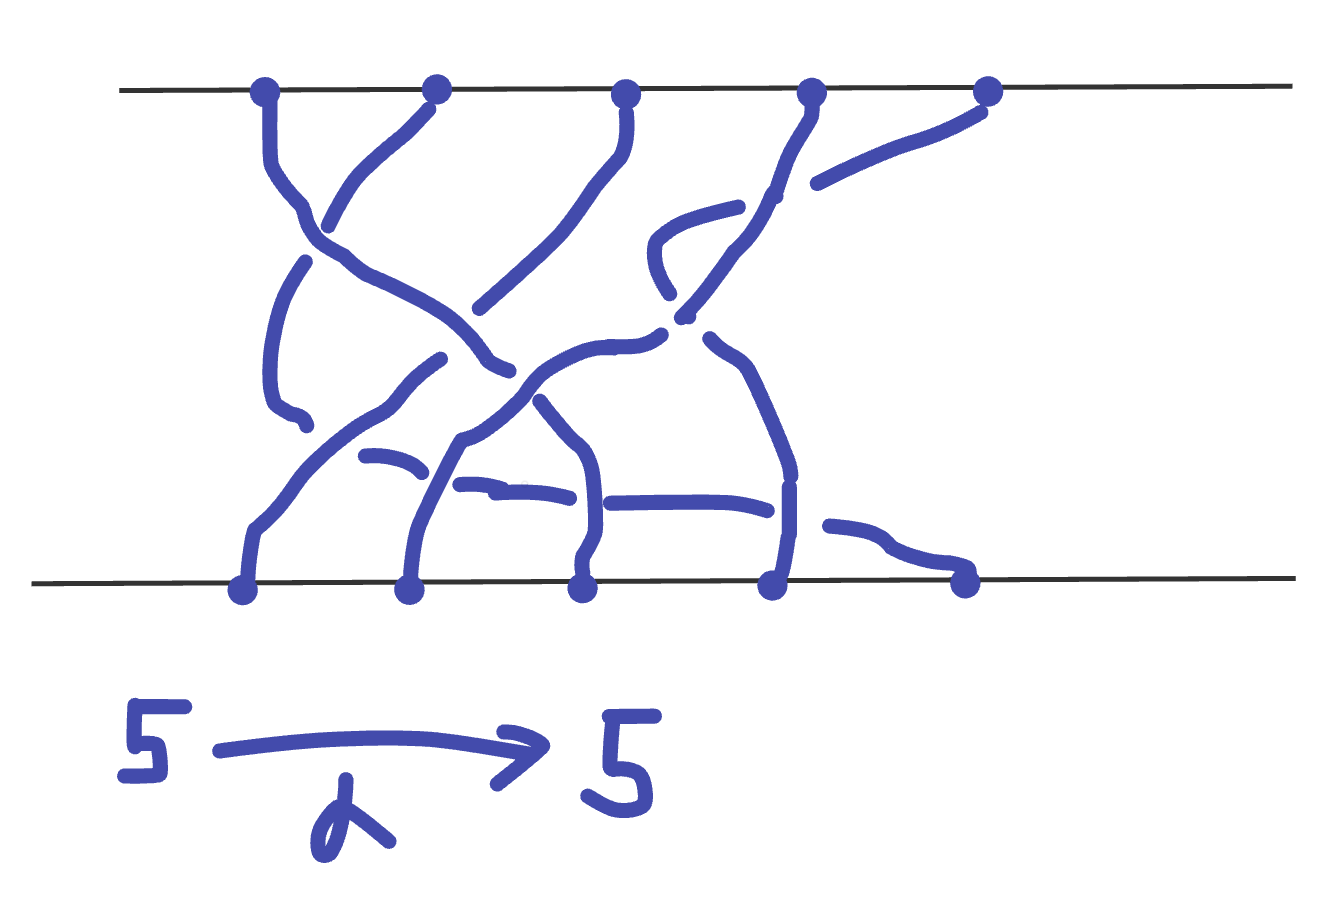
\includegraphics[scale=0.2]{braid1.png}
  \end{center}
  on $n$ strings can be viewed as an element of the Artin braid group $\mathcal{B}_n$ with generators $s_1, \ldots, s_{n - 1}$
  and the following relations:
  \begin{itemize}
    \item $s_i s_j = s_j s_i$ for $j < i - 1$,
    \item $s_{i + 1} s_i s_{i + 1} = s_i s_{i + 1} s_i$
  \end{itemize}
  where $s_i$ is a braid visualised the following way:
  \begin{center}
  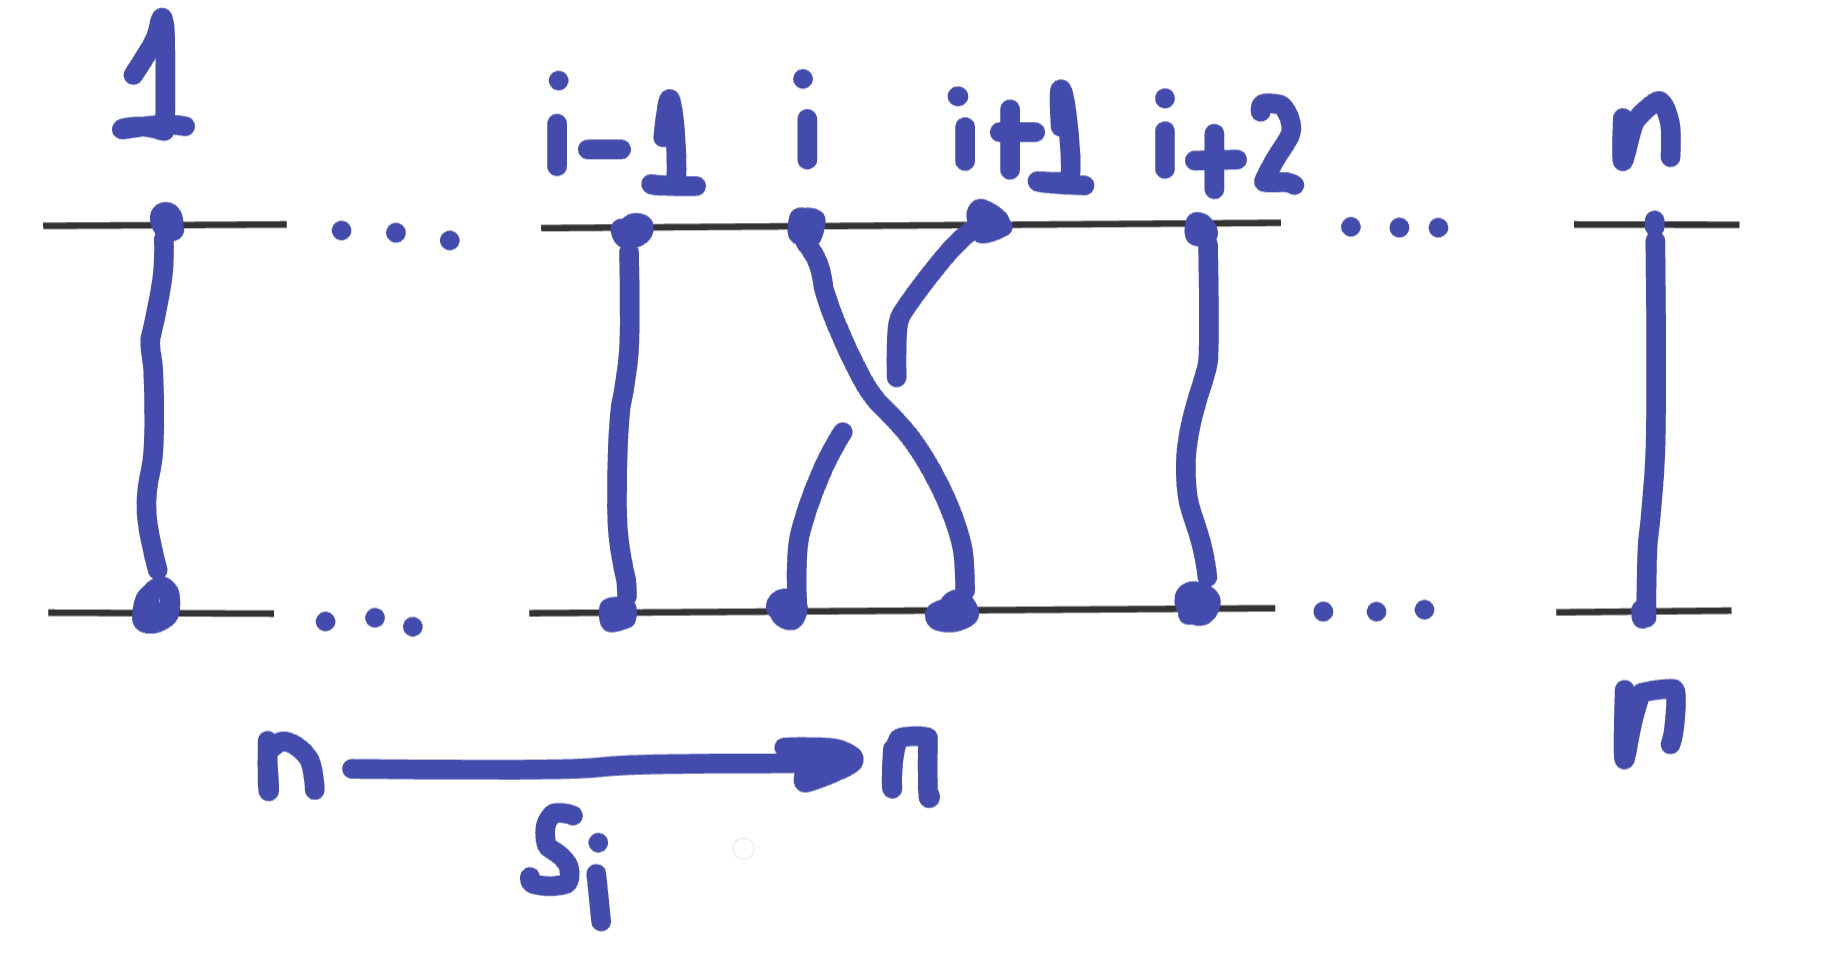
\includegraphics[scale=0.2]{braid2.png}
  \end{center}
  Composition of braids is multiplication is given by multiplication in $\mathcal{B}_n$:
  \begin{center}
  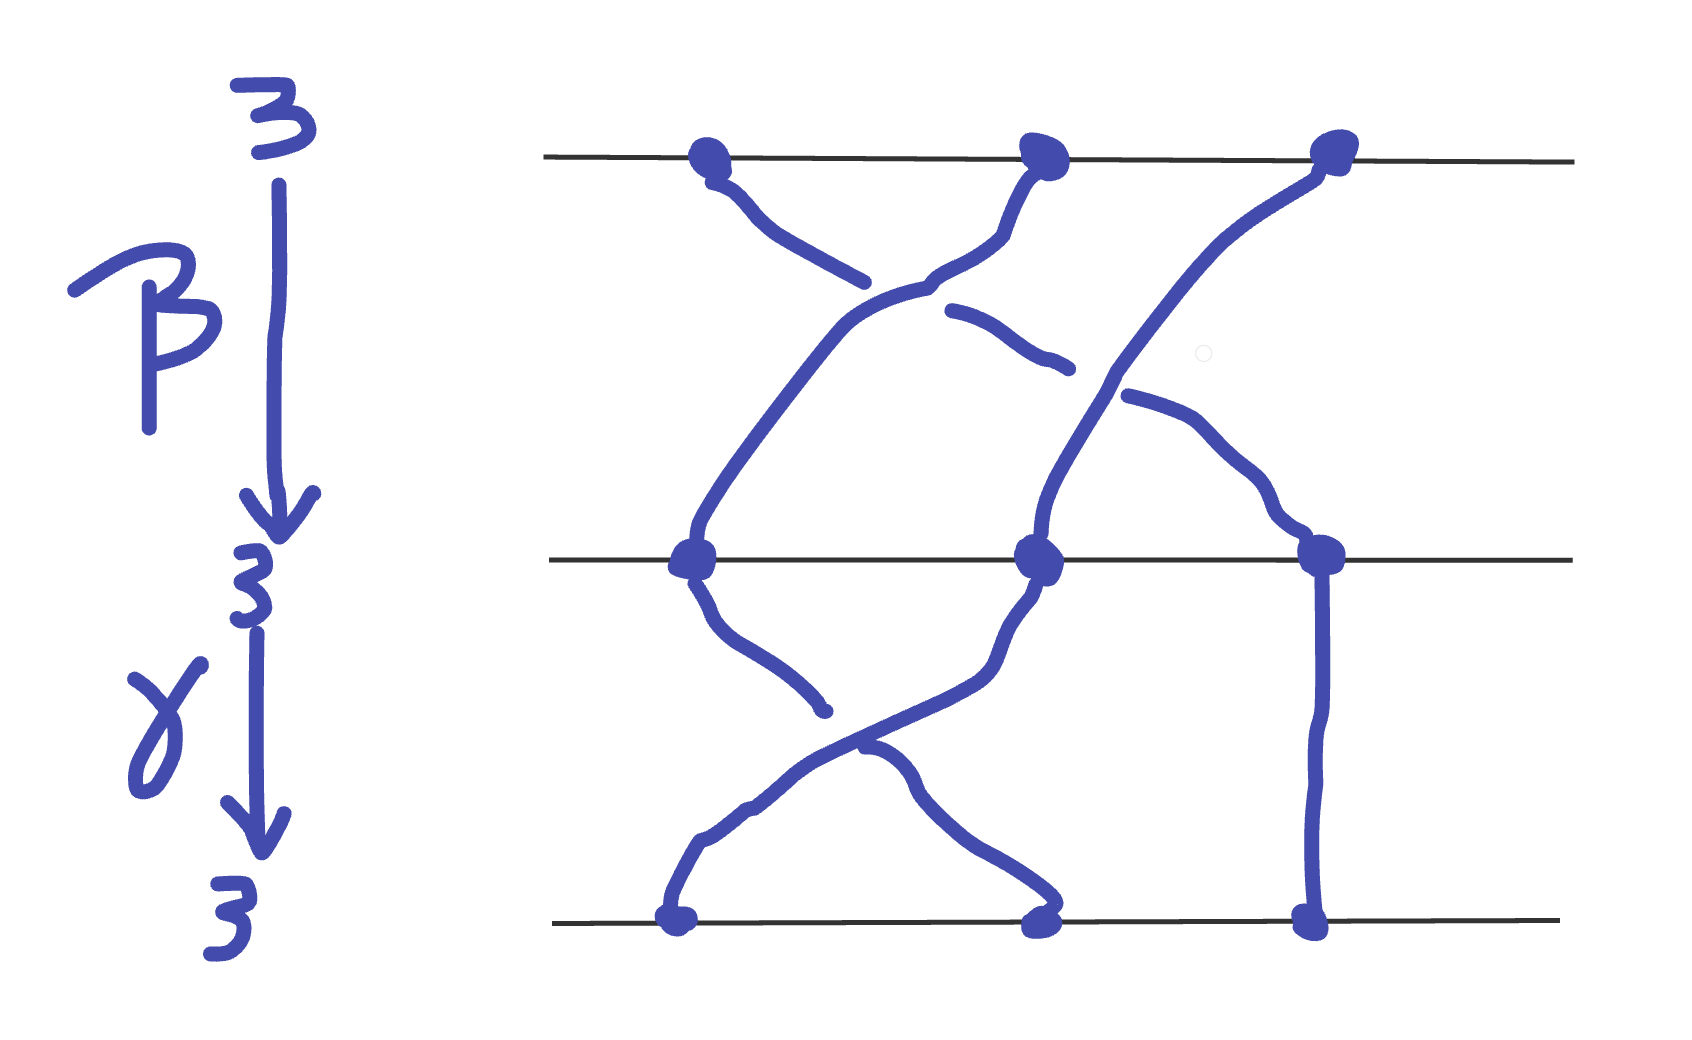
\includegraphics[scale=0.2]{braid3.png}
  \end{center}
  The tensor product of braids adds the numbers of strings by placing one braid next to the other longitudianlly:
  \begin{center}
  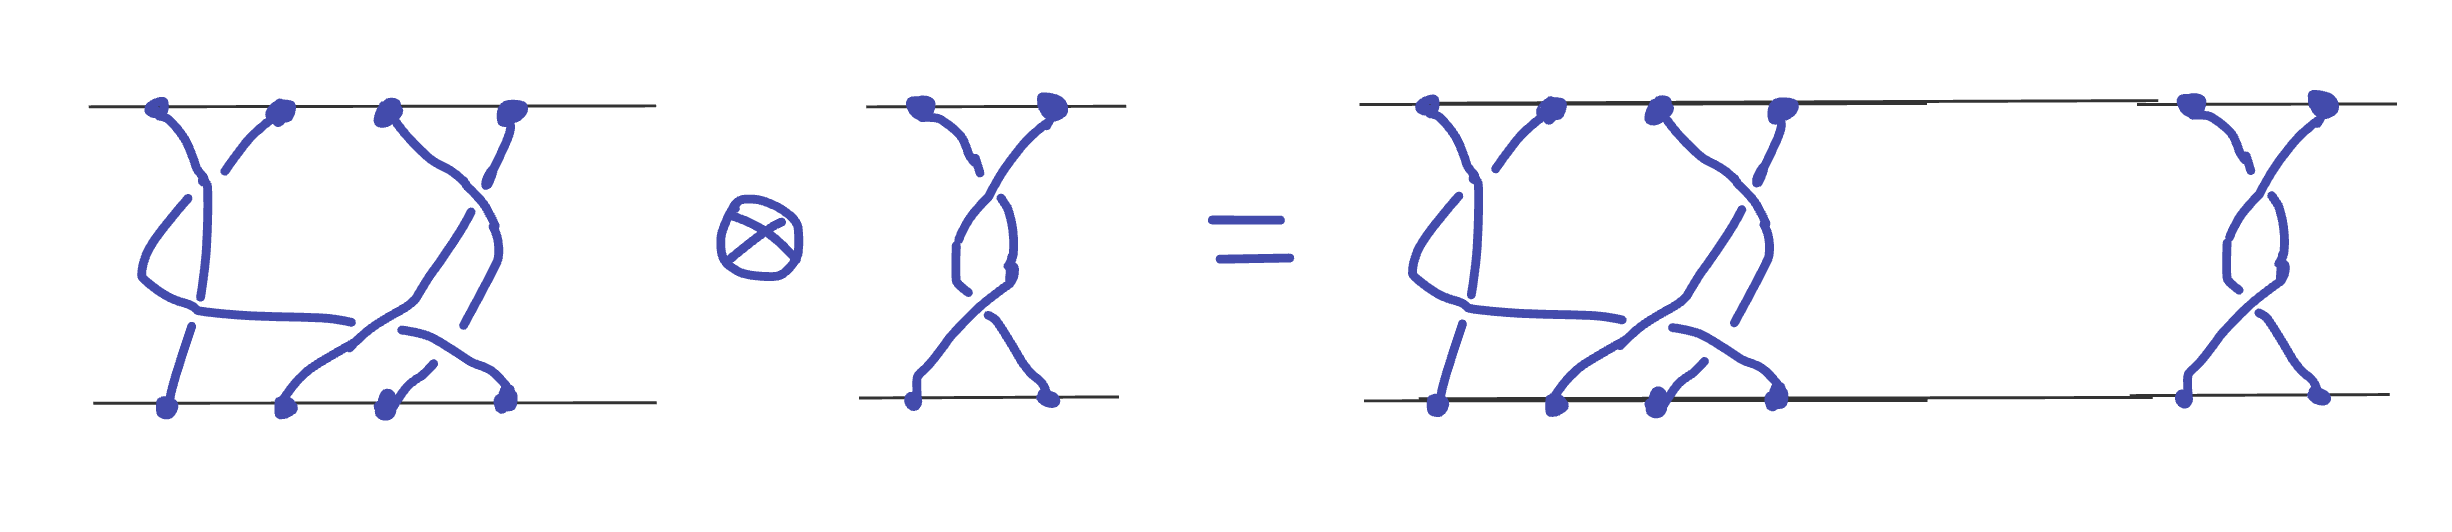
\includegraphics[scale=0.3]{braid4.png}
  \end{center}
\end{example}
Therefore $\mathcal{B}$ is a strict monoidal category. A braiding $c_{m,n} : m + n \to n + m$ is given by crossing the first $m$ strings over the remaining $n$:
  \begin{center}
  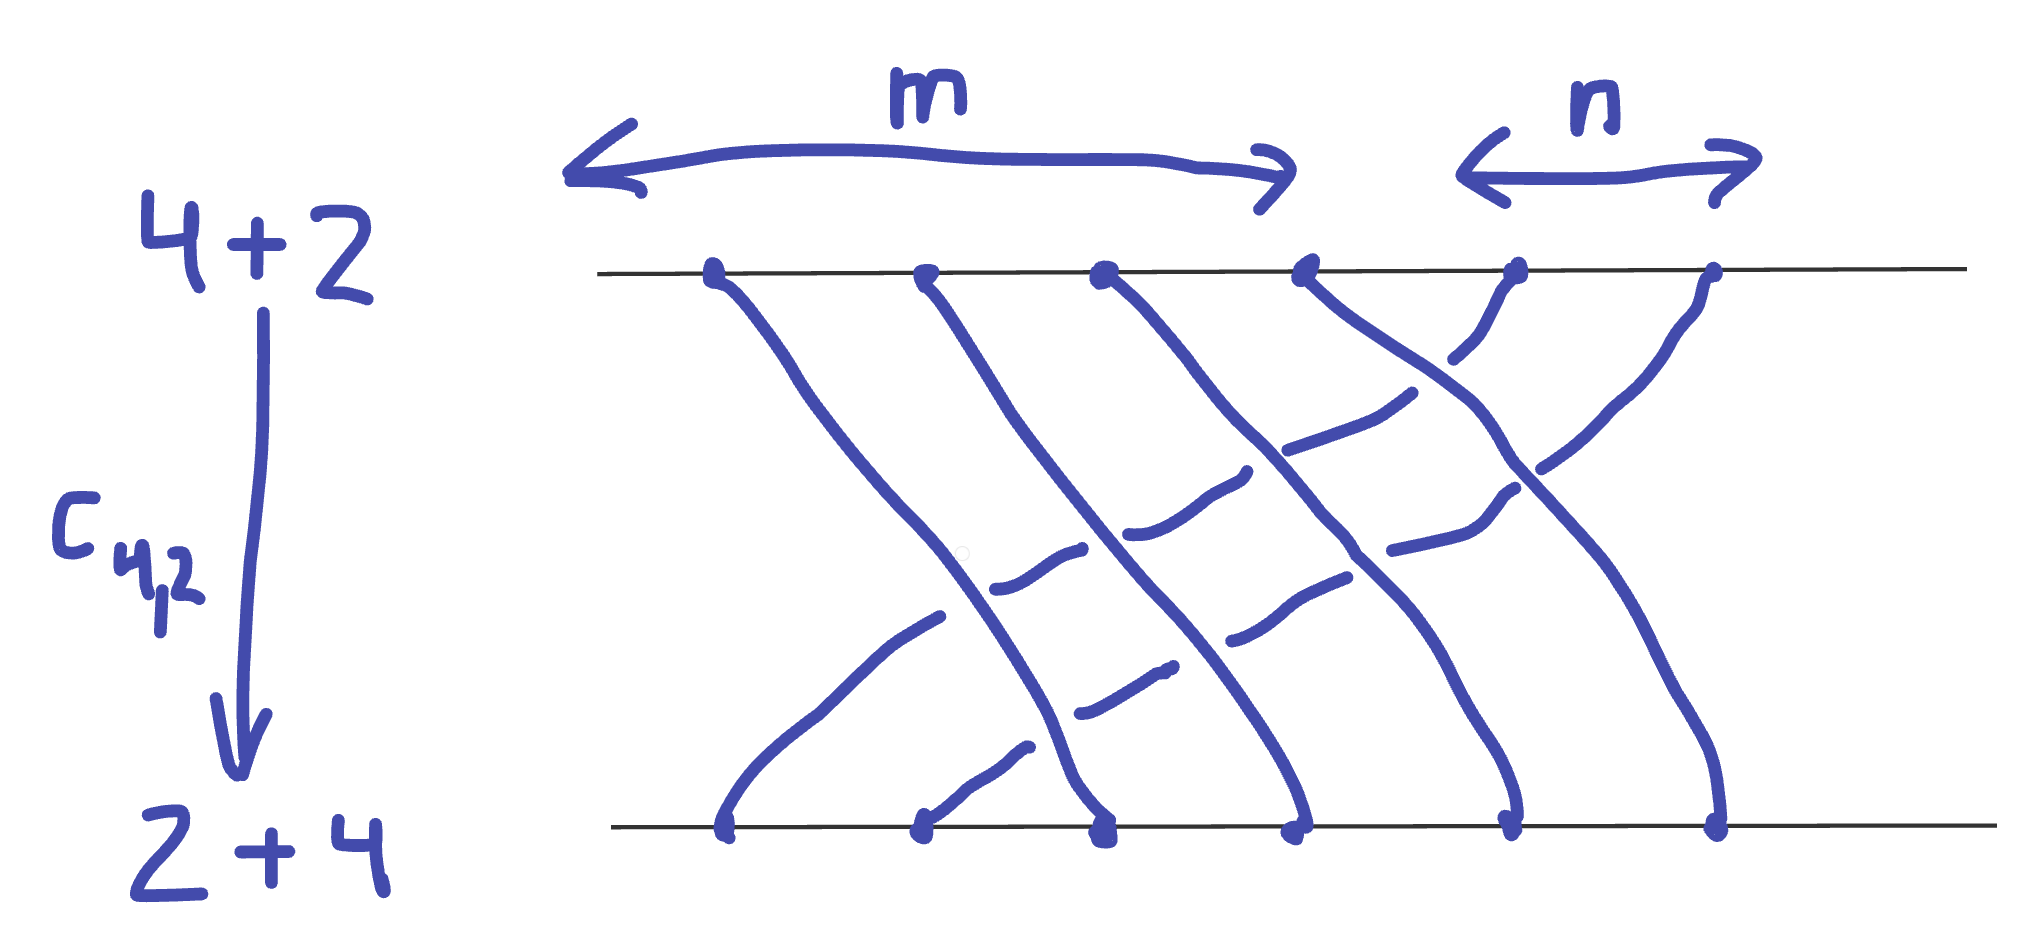
\includegraphics[scale=0.25]{braid5.png}
  \end{center}

\begin{example}
  The category ${\bf Mod}_R$ of modules over a commutative ring $R$ is a symmetric monoidal category with tensor product $\otimes_R$
  and symmetry $\sigma_{A, B} : A \otimes_R B \to B \otimes_R A$.
\end{example}

\begin{example}
  Let $A$ be an $R$-algebra, if $M$ and $N$ are $A$-modules, there is an $A$-module structure on $M \otimes_R N$ is given by:
  \[
  a \cdot (m \otimes n) = \sum \limits_{(a)} a_{(1)} m \otimes a_{(2)} n.
  \]
  Thus ${\bf Mod}_R(A)$ is a monoidal category wuth $\otimes_R$. ${\bf Mod}_R(A)$ is symmetric if $A$ is commutative, but we will be interested
  in a non-commutative $A$. A braiding $c_{M,N} : M \otimes_R N \to N \otimes_R M$, in particular, gives a morphism
  $c_{A,A} : A \otimes_R A \to A \otimes_R A$, which, in turn, gives an element $\gamma = c_{A, A} (1 \otimes 1) \in A \otimes A$.

  Conversely, each element $\gamma = \Sigma_i u_i \otimes v_i \in A \otimes A$ determines a natural transformation with components
  $c_{M,N} : M \otimes_R N \to N \otimes_R M$ via the formula:
  \[
  c_{M,N}(m \otimes n) = \sum \limits_{i} (u_i n) \otimes (v_i m).
  \]
  This is a bijection, as can be seen from the below diagram, where $\hat{m} : A \to M$ is the unique module morphism such that 
  $\hat{m}(1) = m$:
  \[
  \begin{tikzcd}
    R \otimes_R R \ar[r, "\eta"] & A \otimes_R A \ar[d, "\hat{m} \otimes \hat{n}"'] \ar[r, "c_{A,A}"] & A \otimes_R A \ar[d, "\hat{n} \otimes \hat{m}"] \\
    & M \otimes_R N \ar[r, "c_{M,N}"'] & N \otimes_R M
  \end{tikzcd}
  \]
  To make each $c_{M,N}$ to be an isomorphism we need $\gamma \in A \otimes_R A$. We also need each $c$ to be a module morphism:
  \[
  c(a \cdot (m \otimes n)) = c(\sum \limits_{(a)} (a_{(1)} m) \otimes (a_{(2)} n)) = \sum \limits_{(a)} \sum \limits_{i} (u_i a_{(2)} n) \otimes (v_i a_{(1)} m)
  \]
  to be equal to
  \[
  a \cdot c(m \otimes n) = a \cdot \sum \limits_{i} (u_i n) \otimes (v_i m) = \sum \limits_{(a)} \sum \limits_{i} (a_{(1)} u_i n) \otimes (a_{(2)} v_i m).
  \]
  Regarding $\gamma \in A \otimes_R A$ as a morphism $\gamma : R \to A \otimes_R A$, whose value at $1 \in R$ is the given $\gamma$,
  we can express this condition diagrammatically the following way (the B0 condition):
  \[
  \begin{tikzcd}
    A \ar[r, "\gamma \otimes \delta"] & A^{\otimes 4} \ar[r, shift left, "\sigma_{1423}"] \ar[r, shift right, "\sigma_{3142}"'] & A^{\otimes 4} \ar[r, "\mu \otimes \mu"] & A^{\otimes 2}
  \end{tikzcd}
  \]
  For a braiding, we require two more conditions:
  \begin{center}
    $c_{M, N \otimes L}(m \otimes n \otimes l) = (1_N \otimes c_{M,L}) (c_{M,N} \otimes 1_L)(m \otimes n \otimes l)$,

    $c_{M \otimes N, L}(m \otimes n \otimes l) = (c_{M,L} \otimes 1_N)(1_M \otimes c_{N,L})(m \otimes n \otimes l)$.
  \end{center}
  that is,
  \begin{center}
    $\sum \limits_{i,(u_i)} u_{i(1)} n \otimes u_{i(2)} l \otimes v_i m = \sum \limits_{i,j} u_i n \otimes u_j l \otimes v_j v_i m$,

    $\sum \limits_{i,(v_i)} u_i l \otimes v_{i(1)} m \otimes v_{i(2)} n = \sum \limits_{i,j} u_{j} u_i l \otimes v_j m \otimes v_i n$.
  \end{center}
  These are equivalent to the following conditions respectively:
  \begin{center}
      $\sum \limits_{i,(u_i)} u_{i(1)} n \otimes u_{i(2)} l \otimes v_i m = \sum \limits_{i,j} u_i \otimes u_j \otimes v_j v_i$,

      $\sum \limits_{i,(v_i)} u_i l \otimes v_{i(1)} m \otimes v_{i(2)} n = \sum \limits_{i,j} v_j v_i \otimes u_j \otimes u_j$.
  \end{center}
  Diagrammatically, those conditions correspond to the following ones ((B1) and (B2) respectively).
  \[
  \begin{tikzcd}
    R \ar[r, "\gamma \otimes \gamma"] \ar[d, "\gamma"'] & A^{\otimes 4} \ar[r, "\sigma_{1342}"] & A^{\otimes 4} \ar[d, "1 \otimes 1 \otimes \mu"] \\
    A^{\otimes 2} \ar[rr, "\delta \otimes 1"'] && A^{\otimes 3}
  \end{tikzcd}
  \]
  \[
  \begin{tikzcd}
  R \ar[r, "\gamma \otimes \gamma"] \ar[d, "\gamma"'] & A^{\otimes 4} \ar[r, "\sigma_{3142}"] & A^{\otimes 4} \ar[d, "\mu \otimes 1 \otimes 1"] \\
  A^{\otimes 2} \ar[rr, "1 \otimes \delta"'] && A^{\otimes 3}
  \end{tikzcd}
  \]

  Thus one can define a braiding element for a bialgebra $A$ to be an invertible element $\gamma \in A \otimes_R A$.

  A \emph{braided bialgebra}, or a \emph{quasitriangular bialgebra}, is a bialgebra equipped with a braiding element 
  $\gamma \in A \otimes_R A$. A braiding element $\gamma$ is called a \emph{symmetry element} when 
  $\gamma^2 = 1 \in A \otimes_R A$. Symmetry elements are in bijection with symmetries on ${\bf Mod}_R(A)$. A \emph{symmetric bialgebra},
  or a \emph{triangular algebra}, is a bialgebra equipped with a symmetry element.

  Let us point out that the conditions (B1) and (B2) can be reworded differently if $A$ is Cauchy as an $R$-module. In this case, 
  elements $\gamma = \sum \limits_{i} u_i \otimes v_i \in A \otimes_R A$ are in bijection with $R$-module morphisms 
  $g : A^* \to A$ with the following formula:
  \[
  \gamma = (R \xrightarrow{d} A^* \otimes_R A \xrightarrow{g \otimes 1_A} A \otimes_R A)
  \]
  (B1) says that $g$ preserves comultiplication, whilst (B2) says that $g$ preserves multiplication. In fact, if $\gamma$ is a braiding
  element, $g : A^* \to {A'}^{op}$ is a bialgebra morphism; preservation of unit and counit follows from $c_{M,I} = c_{I, M} = 1_M$.

  Let us consider the translation of (B2) to $g$. Let us start with the following diagram
  \[
  \begin{tikzcd}
    R \ar[rr, "d"] \ar[dd, "d"'] && A^{*} \otimes_R A \ar[rr, "1 \otimes d \otimes 1"] && A^* \otimes_R A^* \otimes_R A \otimes_R A \ar[dd, "\delta^* \otimes 1 \otimes 1"] \\
    \\
    A^* \otimes_R A \ar[rrrr, "1 \otimes \delta"'] &&&& A^* \otimes_R A \otimes_R A
  \end{tikzcd}
  \]
  for $\delta$, which is the multiplication for $A^*$. To prove $g$ preserves multiplication is to prove:
  \[
  \begin{tikzcd}
  A^* \otimes_R A^* \ar[d, "d^*"'] \ar[r, "g \otimes g"] & A \otimes_R A \ar[r, "\sigma"] & A \otimes_R A \ar[d, "\mu"] \\
  A^* \ar[rr, "g"] && A
  \end{tikzcd}
  \]
  This is equivalent to proving the legs are equal after applying $\underline{\:\:} \otimes_R A \otimes_R A$ and composing with
  \[
  R \xrightarrow{d} A^* \otimes_R A^* \xrightarrow{1 \otimes d \otimes 1} A^* \otimes_R A^* \otimes_R A \otimes_R A.
  \]
  Thus we have:
  \[
  \begin{tikzcd}
    R \ar[r, "d"] & A^* \otimes_R A^* \ar[d, "1 \otimes \delta"'] \ar[rr, "1 \otimes d \otimes 1"] && A^* \otimes_R A^* \otimes_R A \otimes_R A \ar[rr, "g \otimes g \otimes 1 \otimes 1"] && A^{\otimes 4} \ar[r, "\sigma"] & A^{\otimes 4} \ar[d, "\mu \otimes 1 \otimes 1"] \\
    & A^* \otimes_R A \otimes_R \ar[rrrrr, "g \otimes 1 \otimes 1"'] &&&&& A^{\otimes 3}
  \end{tikzcd}
  \]
\end{example}

Let $\mathcal{V}$ be a braided tensor category, a twist for $\mathcal{V}$ is a family of isomorphisms $\theta_A : A \to A$
such that $\theta_I = 1_I$ and
\[
\begin{tikzcd}
  A \otimes B \ar[r, "c_{A,B}"] \ar[d, "\theta_{A \otimes B}"'] & B \otimes A \ar[d, "\theta_B \otimes \theta_A"] \\
  A \otimes B & B \otimes A \ar[l, "c_{B,A}"]
\end{tikzcd}
\]

A \emph{balanced tensor category} is a braided monoidal category with a choice of a twist.

\begin{example} The braid category $\mathcal{B}$ is canonically balanced. The twist $\theta_n : n \to n$ is obtained by taking
  $n$ vertical parallel strings with ends tied to two horizontal parallel rods, and rotating the bottom rod through a full $2 \pi$
  twist in the right-hand screw direction with thumb vertical. Then $\theta_0$, $\theta_1$ are identities, while $\theta_2$ is:
  \begin{center}
  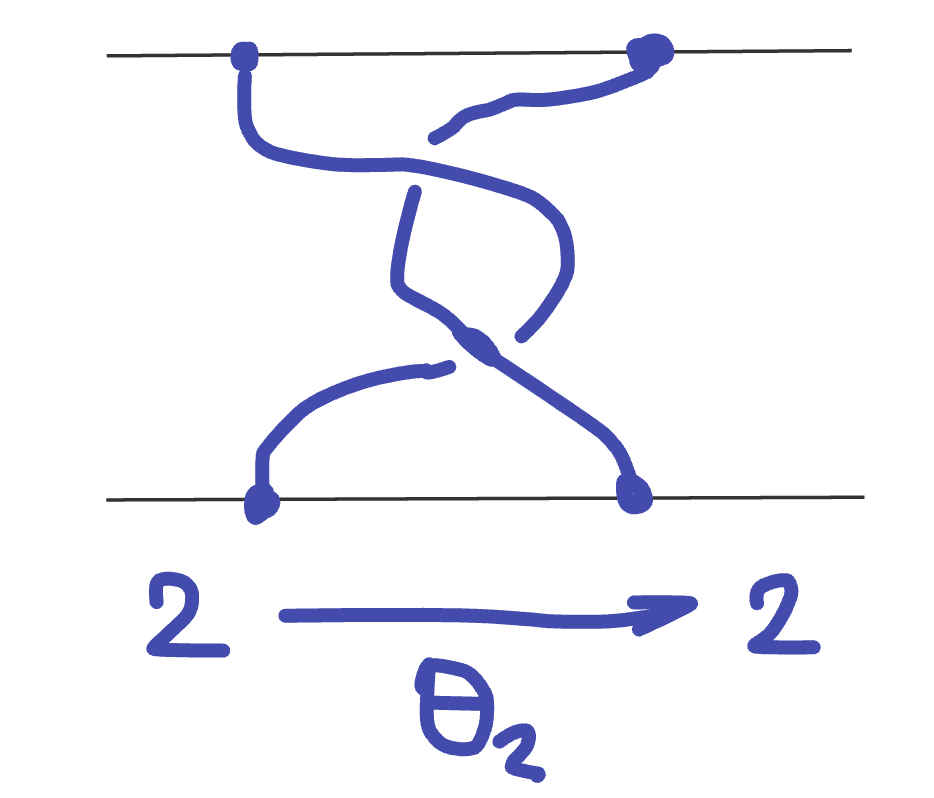
\includegraphics[scale=0.25]{braid6.png}
  \end{center}
\end{example}

\begin{example} There is a monoidal category $\widetilde{\mathcal{B}}$, which is defined similarly to $\mathcal{B}$,
  except that the arrows are braids on ribbons (instead of strings), and it is permissible to twist the ribbons through full
  $2 \pi$ turns:
  \begin{center}
  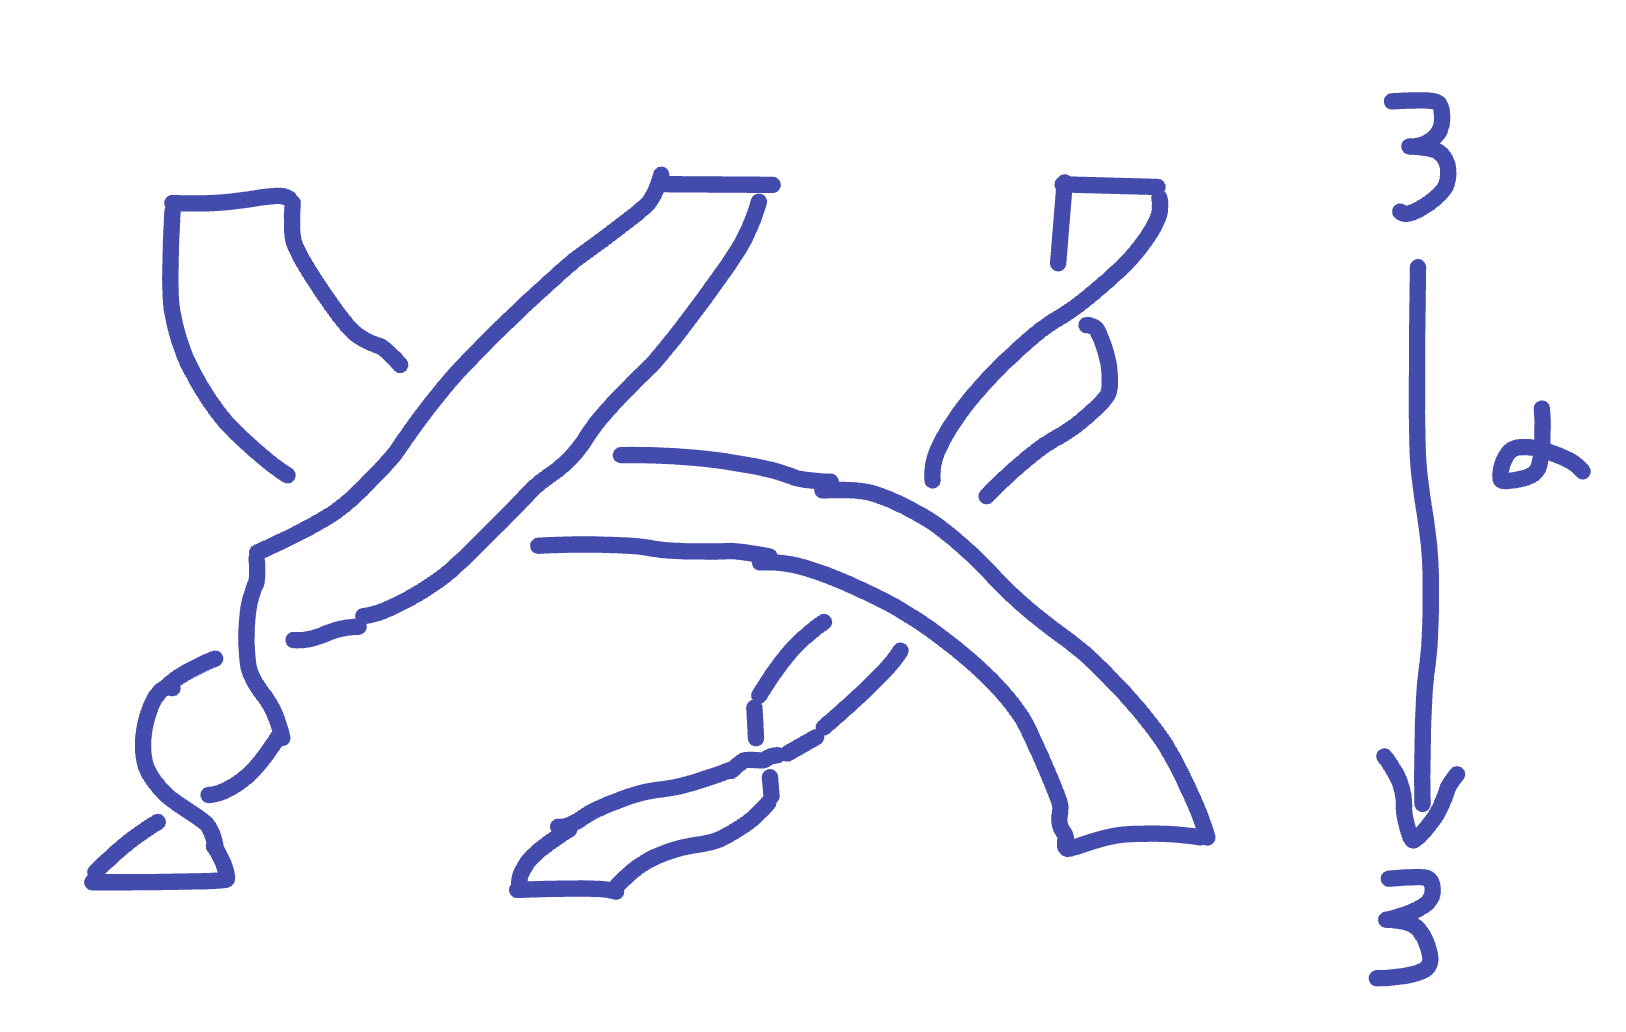
\includegraphics[scale=0.2]{ribbons1.png}
  \end{center}
  The homsets $\widetilde{\mathcal{B}}(n,n) = \widetilde{\mathcal{B}}_n$ are groups under composition. A presentation
  of this group $\widetilde{\mathcal{B}}_n$ is given by generators $s_1, \ldots, s_n$, where $s_1, \ldots,s_{n - 1}$
  satisfy the relations from the Artin braid group $\mathcal{B}_n$, whereas $s_1, \ldots, s_n$ satisfy the extra relation
  \[
  s_{n - 1} s_n s_{n - 1} s_n = s_n s_{n - 1} s_n s_{n - 1}
  \]
  where $s_n$ is depicted as follows:
  \begin{center}
  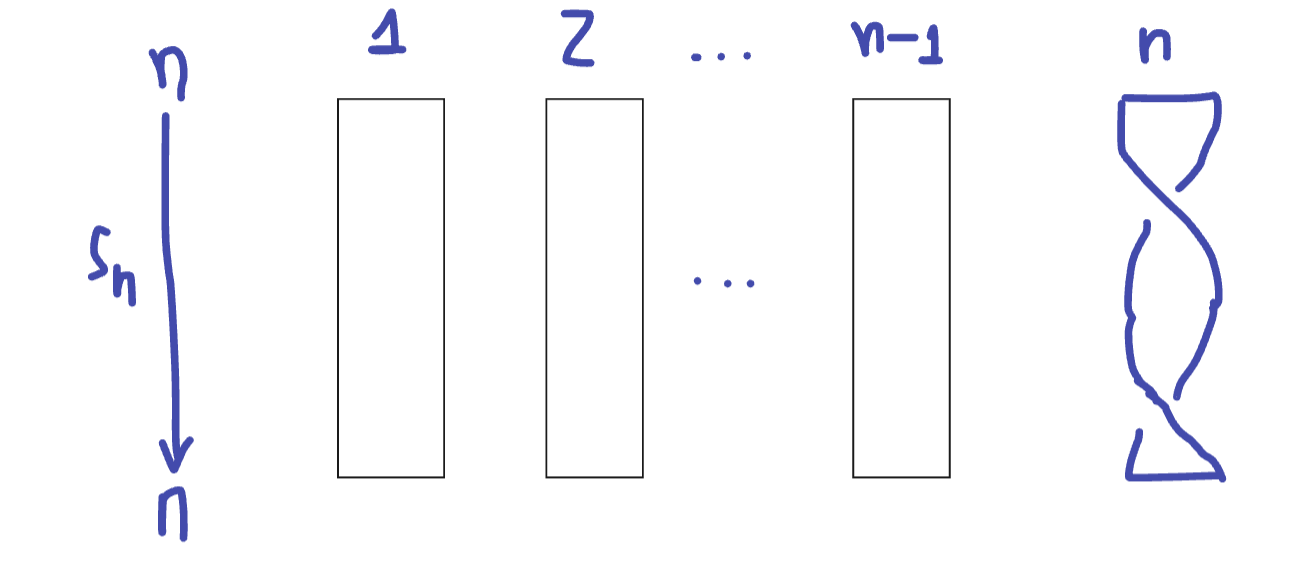
\includegraphics[scale=0.35]{ribbons2.png}
  \end{center}
  Composition in $\widetilde{\mathcal{B}}$ is vertical stacking of diagrams, and tensor product for $\widetilde{\mathcal{B}}$
  is horizontal placement of diagrams, much as for $\mathcal{B}$. The braiding $c_{m,n} : m + n \to n + m$ for $\widetilde{\mathcal{B}}$
  is obtained by placing the first $m$ ribbons over the remaining $n$ without introducing any twists. Now the twist $\theta_n : n \to n$
  for $\widetilde{\mathcal{B}}$ is obtained by regarding the two boundary edges of the ribbons as extra strings and taking $\theta_{2n} : 2n \to 2n$
  in $\mathcal{B}$. Therefore, we have the following $\widetilde{\mathcal{B}}$:
  \begin{center}
  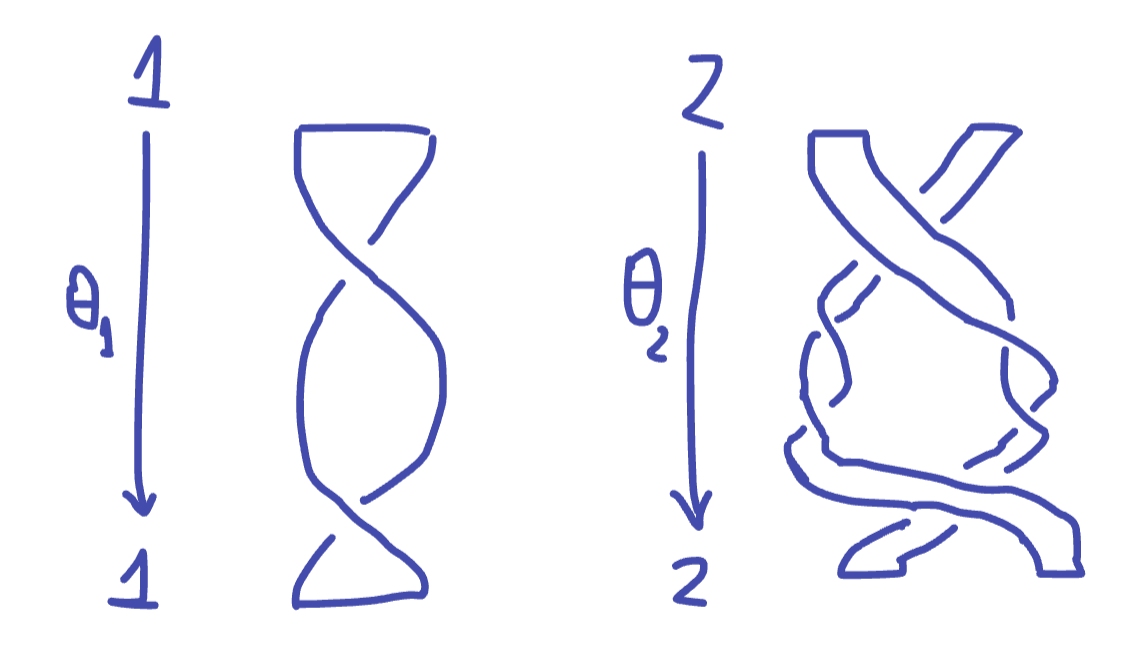
\includegraphics[scale=0.3]{ribbons3.png}
  \end{center}
\end{example}
\begin{example}
  Let $A$ and $B$ be Abelian groups and let $f : A \times A \to B$ be a bilinear function. Then there is a balanced strict monoidal category
  $\mathcal{C}_f$ is constructed the following way: the objects are elements of $A$, the homset $\mathcal{C}_f(x, y)$ is empty unless
  $x = y$ and $\mathcal{C}_f(x,x) = B$. The tensor product is given by
  \[
  (x \xrightarrow{\alpha} x) \otimes (y \xrightarrow{\beta} y) = (x+y \xrightarrow{\alpha + \beta} x + y).
  \]
  The braiding is $c_{x,y} = f(x,y) : x + y \to y + x$ and the twist is given by $\theta_X = f(x,x) : x \to x$.
\end{example}
\begin{example}
  Let $A$ be a braided $R$-algebra with braiding element:
  \[
  \gamma = \sum \limits_{i \in I} u_i \otimes v_i \in A \otimes_R A.
  \]
  A \emph{twist element} for $A$ is an invertible central element $\tau \in A$ such that $\varepsilon(\tau) = 1$
  \[
  \delta(\tau) = \sum \limits_{i,j} (u_i \tau v_j) \otimes (v_i \tau u_i).
  \]
  The above equation is diagrammatically presented the following way:
  \[
  \begin{tikzcd}
    R \ar[dd, "\tau"'] \ar[rr, "\gamma \otimes \tau \otimes \tau \otimes \gamma"] && A^{\otimes 6} \ar[rr, "\sigma_{136245}"] && A^{\otimes 6} \ar[d, "\mu \otimes 1 \otimes \mu \otimes 1"] \\
    &&&& A^{\otimes 4} \ar[d, "\mu \otimes \mu"] \\
    A \ar[rrrr, "\delta"] &&&& A^{\otimes 2}
  \end{tikzcd}
  \]
\end{example}

Twist elements $\tau$ for $A$ are in bijection with twists $\theta$ for the braided monoidal category ${\bf Mod}_R(A)$.
Naturality of $\theta_M : M \to M$ means it has the form of $\theta_M(m) = \tau m$ for some $\tau \in A$. To make $\theta_M$ an $A$-module morphism,
$\tau$ should be central, i.e. $\tau \cdot a = a \cdot \tau$ for all $a \in A$.

A \emph{balanced algebra} is a braided bialgebra with a twist.

\subsection{Exercises}

\begin{exercise} Let $\mathcal{V}$ be a braided monoidal category, then:
  \begin{enumerate}
    \item $c_{A,I} = c_{I, A} = 1_A$ and the following diagram commutes for any $A, B, C \in \mathcal{V}$ (modulo associativity):
    \[
    \begin{tikzcd}
      & A \otimes C \otimes B \ar[rr, "c_{A,C} \otimes 1_B"] && C \otimes A \otimes B \ar[dr, "1_C \otimes c_{A,B}"]\\
      A \otimes B \otimes C \ar[dr, "c_{A, B} \otimes 1_C"'] \ar[ur, "1_A \otimes c_{B,C}"] &&&& C \otimes B \otimes A \\
      & B \otimes A \otimes C \ar[rr, "1_B \otimes c_{A,C}"'] && B \otimes C \otimes A \ar[ur, "c_{B, C} \otimes 1_A"']
    \end{tikzcd}
    \]
    \item For a braided bialgebra $A$ and $\mathcal{V} = {\bf Mod}_R(A)$, interpret the properties of $c$ from the previous item in terms of the braiding
    element $\gamma \in A \otimes_R A$.
    \item Draw a diagram of braids, expressing the hexagonal diagram of the first item in the braid category $\mathcal{B}$.
  \end{enumerate}
\end{exercise}

\begin{proof}
  $ $

  \begin{enumerate}
    \item One has $c_{A,I} = c_{A,I} \circ c_{A,I}$ from the below triangle:
    \[
    \begin{tikzcd}
      A \cong A \otimes I \otimes I \ar[r, "c_{A, I \otimes I}"] \ar[d, "c_{A,I} \otimes 1_I"'] & I \otimes I \otimes A \cong A \\
      A \cong I \otimes A \otimes I \ar[ur, "1_I \otimes c_{A,I}"']
    \end{tikzcd}
    \]
    $c_{A,I}$ is invertible, so $c_{A,I} = 1_A$, and the proof for $c_{I,A}$ is similar. The second condition is proved by dividing the goal diagram
    to the commutative subdiagrams:
      \[
    \begin{tikzcd}
      & A \otimes C \otimes B \ar[rr, "c_{A,C} \otimes 1_B"] && C \otimes A \otimes B \ar[dr, "1_C \otimes c_{A,B}"]\\
      A \otimes B \otimes C \ar[dr, "c_{A, B} \otimes 1_C"'] \ar[urrr, "c_{A \otimes B, C}"'] \ar[ur, "1_A \otimes c_{B,C}"] &&&& C \otimes B \otimes A \\
      & B \otimes A \otimes C \ar[rr, "1_B \otimes c_{A,C}"'] \ar[urrr, "c_{B \otimes A, C}"] && B \otimes C \otimes A \ar[ur, "c_{B, C} \otimes 1_A"']
    \end{tikzcd}
    \]
    \item
    \item 
  \end{enumerate}
\end{proof}

\section{Internal homs and duals}

Let $\mathcal{V}$ be a monoidal category and let $A$ and $B$ be objects in $\mathcal{V}$. A \emph{left internal hom} for $A$ and $B$
is an object $[A, B]$ along with the \emph{evaluation arrow} $e_A : [A, B] \otimes A \to B$ such that for all arrows $f : C \otimes A \to B$
there exists a unique arrow $\hat{f} : C \to [A, B]$ such that the following holds:
\[
\begin{tikzcd}
  {[}A, B{]} \otimes A \ar[rr, "e_A"] && B \\
  C \otimes A \ar[u, "\hat{f} \otimes 1_A"] \ar[urr, "f"'] 
\end{tikzcd}
\]
Thus there is a natural bijection:
\begin{center}
  $\mathcal{V}(C, [A, B]) \cong \mathcal{V}(C \otimes A, B)$

  $g \mapsto e_A \circ (g \otimes 1_A)$
\end{center}

A monoidal category is \emph{left-closed} if each pair of objects has a left internal hom. If $f : C \to A$ and $g : B \to D$ are arrows in $\mathcal{V}$, provided
$\mathcal{V}$ is monoidal closed, then there is a unique arrow:
\[
[f, g] : [A, B] \to [C, D]
\]
such that:
\[
\begin{tikzcd}
  \IntHom{A,B} \otimes C \ar[d, "1 \otimes f"'] \ar[rr, "\IntHom{f,g} \otimes 1"]  && \IntHom{C,D} \otimes C  \ar[d, "e_C"] \\
  \IntHom{A,B} \otimes A \ar[r, "e_A"'] & B \ar[r, "g"'] & D
\end{tikzcd}
\]
Therefore the internal hom is a functor $[\underline{\:\:},\underline{\:\:}] : \mathcal{V}^{op} \otimes \mathcal{V} \to \mathcal{V}$.

The internal hom for $A$ and $B$ is unique up to isomorphism. An internal hom for $I$ and $A$ always exists since we have
$[I, A] = A$ with $e_A = r_A : A \otimes I \to A$.

If $B, C$ and $A \otimes B, C$ have internal homs, so do $A, [B, C]$:
\[
[A, [B, C]] = [A \otimes B, C]
\]
with $a_A = \hat{e_{A \otimes B}} : [A \otimes B, C] \otimes A \to [B, C]$.

There is a composition arrow: $[B, C] \otimes [A, B] \to [A, C]$ in $\mathcal{V}$ (whenever the corresponding internal homs do exist),
which corresponds to the following composite:
\[
[B, C] \otimes [A, B] \otimes A \xrightarrow{1 \otimes e_A} [B, C] \otimes B \xrightarrow{e_B} C.
\]
A right internal hom is defined dually and is denoted as $[A, B]'$. The right evaluation arrow has the form of $e'_A : A \otimes [A,B]' \to B$.

A monoidal category is \emph{closed} if it has all left and right internal homs.

\begin{example}
  The symmetric monoidal category ${\bf Mod}_R$ of modules over a commutative ring $R$ is closed:
  \[
  [M, N] = [M, N]' = \operatorname{Hom}_R(M, N)
  \]
\end{example}

\begin{example}
  Let $H$ be an $R$-Hopf algebra. Then the tensor category ${\bf Mod}_R(H)$ of $H$-modules with tensor product $\otimes_R$ is left-closed:
  \[
  [M, N] = \operatorname{Hom}_R(M, N)
  \]
  Assume the antipode $\nu$ for $H$ is invertible, then $H'$ becomes a Hopf algebra with antipode $\nu^{-1}$.
  Let $\operatorname{Hom}'_R(M,N)$ denote $\operatorname{Hom}_R(M,N)$ as a left $H'$-module. The forgetful functor 
  ${\bf Mod}_R(H) \to {\bf Mod}_R$ preserves tensors and left/right internal homs.
\end{example}

\begin{example}
  Let ${\bf Ban}$ be the category of Banach spaces over $\mathbb{C}$ and arrows $f : A \to B$ are linear functions such that
  \[
  ||f(a)|| \leq ||a||.
  \]
  One can make ${\bf Ban}$ into a symmetric tensor category by taking tensor products as vector space. The internal hom exists for all Banach spaces,
  which is the Banach space of bounded functions with the usual norm. Thus ${\bf Ban}$ is a symmetric monoidal category.
\end{example}

Let $\mathcal{V}$ be a monoidal category. An object $J$ is \emph{left dualising} when, for each $A$, internal homs 
$[A, J]$ and $[A, J]'$ exist, and the arrow $\omega_A : A \to [[A, J]', J]$ is invertible. Thus $\mathcal{V}$ is left-closed with
\[
[A,B] = [A \otimes [B, J]', J]
\]
since
\[
\mathcal{V}(C, [A \otimes [B,J]',J]) \cong \mathcal{V}(C \otimes A \otimes [B,J]',J) \cong \mathcal{V}(C \otimes A, [[B,J]',J]) \cong \mathcal{V}(C \otimes A, B).
\]
The concept of right dualising object is defined similarly.

\begin{example}
  Let ${\bf k}$ be a field. A \emph{quadratic algebra} is a pair $(V, R)$ where $V$ is a finite-dimensional vector space and $R$ is a subspace of $V \otimes V$. 
  A quadratic algebra morphism $f : (V, R) \to (W, S)$ is a linear function $f : V \to W$ such that
  \[
  (f \otimes f)(R) \subseteq S
  \]
  Write $\mathcal{Q}\mathcal{A}$ for the category of quadratic algebras. Each quadratic algebra $(V, R)$ determines an actual algebra:
  \[
  T(V)/R
  \]
  where $T(V)$ is the tensor algebra on $V$. $\mathcal{Q}\mathcal{A}$ is an SMC with a symmetric tensor product given:
  \[
  (V, R) \otimes (W, S) = (V \otimes W, \sigma_{1324}(R \otimes S))
  \]
  The unit object is $I = ({\bf k}, {\bf k} \otimes {\bf k})$.
  The claim is that $J = ({\bf k}, 0)$ is a dualising object. Observe that:
  \[
  [(V, R), J] = (V^*, R^{\bot})
  \]
  where $V^* = \operatorname{Hom}_{\bf k}(V, {\bf k})$ and $R^{\bot}$ is the kernel of the composite surjection:
  \[
  V^* \otimes V^* \xrightarrow{\cong} (V \otimes V)^* \xrightarrow{i^*} R^*
  \]
  where $i : R \to V \otimes V$ being inclusion. It follows that $R$ is the kernel of
  \[
  \begin{tikzcd}
    V \otimes V \ar[rr, "\omega"]  &&V^{**} \otimes V^{**} \ar[rr, "\cong"] && (V^{*} \otimes V^{*})^{*} \ar[rr, "i^*"] && R^{\bot *}
  \end{tikzcd}
  \]
  so we have an isomorphism:
  \[
  \omega : (V, R) \cong (V^{**}, R).
  \]
  The quadratic algebra which we identify with the quantum plane $\mathbb{A}^{2|0}_q$ is
  \[
  \mathbb{A}^{2|0}_q = ({\bf k}^2, (y \otimes x - q x \otimes y))
  \]
  where $x = (1, 0)$, $y = (0, 1) \in {\bf k}^2$. Let $\xi, \eta \in {\bf k}^{2*}$ be the dual basis given by $\xi(x) = \eta(y) = 1$, $\xi(y) = \eta(x) = 0$. Then:
  \[
  (y \otimes x - q x \otimes y)^{\bot} = (\xi \otimes \xi, \eta \otimes \eta, \xi \otimes \eta + q \eta \otimes \xi)
  \]
  as a subspace of ${\bf k}^{2*} \otimes {\bf k}^{2*}$. Hence the quantum superplane arises as the quadratic algebra:
  \[
  \mathbb{A}^{0|2}_q = ({\bf k}^{2*}, (\xi \otimes \xi, \eta \otimes \eta, \xi \otimes \eta + q \eta \otimes \xi)) = [\mathbb{A}^{0|2}_q, J].
  \]
  Notice also that:
  \[
  \mathbb{A}^{0|2}_q \otimes \mathbb{A}^{2|0}_q = ({\bf k}^{2*} \otimes {\bf k}^2, (b \otimes a - q a \otimes b, d \otimes c - q c \otimes d, q^{-1} b \otimes c - q c \otimes b + d \otimes a - a \otimes d)).
  \]
\end{example}

  Let $\mathcal{V}$ be a monoidal category. Write $d, e : B \dashv A$, or just $B \dashv A$, for $A, B \in \mathcal{V}$ and arrows $e : B \otimes A \to I, d : I \to A \otimes B$
  such that the following diagram commutes:
  \[
  \begin{tikzcd}
    A \ar[rr, "d \otimes 1_A"] \ar[drr, equal] && A \otimes B \otimes A \ar[d, "1_A \otimes e"] & B \ar[drr, equal] \ar[rr, "1_B \otimes d"] && B \otimes A \otimes B \ar[d, "e \otimes 1_B"] \\
    && A &&& B 
  \end{tikzcd}
  \]

  $B$ is called a \emph{left dual} for $A$, and $A$ is called a \emph{right dual} for $B$. $e$ is called \emph{the counit}, $d$ is called \emph{the unit}. Duals
  are defined uniquely up to isomorphism.

  A monoidal category is called \emph{left autonomous} when each $A \in \mathcal{V}$ has a left dual $A^*$. Each arrow $f : A \to B$ determines a unique arrow $f^* : B^* \to A^*$
  given by the composite:
  \[
  \begin{tikzcd}
    B^* \ar[rr, "1 \otimes d"] && B^* \otimes A \otimes A^* \ar[rr, "1 \otimes f \otimes 1"] && B^* \otimes B \otimes A^* \ar[rr, "e \otimes 1"] && A^*
  \end{tikzcd}
  \]
  So one makes left dual into a functor $(\underline{\:\:\:})^* : \mathcal{V}^{op} \to \mathcal{V}$. We also have $(A \otimes B)^* \cong B^* \otimes A^*$ 
  and $I^* \cong I$. The monoidal category is \emph{autonomous} when each $A$ has both a left dual $A^*$ and right dual $A^{\vee}$.

  If $\mathcal{V}$ is braided, then each left dual $A^*$ is also a right dual with counit and unit:
  \[
  \begin{tikzcd}
    A \otimes A^{*} \ar[rr, "c_{A,A^*}"] && A^{*} \otimes A \ar[rr, "e"] && I
  \end{tikzcd}
  \]
  \[
  \begin{tikzcd}
    I \ar[rr, "d"] && A \otimes A^{*} \ar[rr, "c^{-1}_{A,A^*}"] && A^{*} \otimes A
  \end{tikzcd}
  \]
  Therefore, $A \cong A^{**}$.

  A \emph{tortile monoidal category} is an autonomous balanced monoidal category, in which twist is related to the dual via the condition:
  \[
  \theta_{A^*} = \theta^*_A : A^* \to A^{*}
  \]
  A left dual $A^*$ for $A$ gives a left internal hom $[A, B] = B \otimes A^*$ with evaluation:
  \[
  e_A = 1 \otimes e : B \otimes A^* \otimes A \to B
  \]
  for each $B \in \mathcal{V}$. A right dual $A^{\vee}$ gives a right internal hom $[A,B]' = A^{\vee} \otimes B$. Thus a left/right autonomous monoidal category
  is left/right-closed.

  \begin{example}
    Let $R$ be a commutative ring $R$, an object $M$ of ${\bf Mod}_R$ a (left) dual if and only if it is Cauchy. ${\bf Prf}_R$ is the full subcategory
    of ${\bf Mod}_R$ consisting of Cauchy $R$-modules. ${\bf Prf}_R$ is closed under $\otimes$, so ${\bf Prf}_R$ is an autonomous monoidal category.
  \end{example}

  \begin{example}
    Let $H$ be an $R$-Hopf algebra. An object $M$ of the monoidal category ${\bf Mod}_R(H)$ has a left dual iff it is Cauchy as an $R$-module; $M^* = \operatorname{Hom}_R(M,R)$.
    If $H$ has an invertible antipode, then each $M$ has a right dual $M^{\vee} = \operatorname{Hom}'_R(M, R)$. Write ${\bf Prf}_R(H)$ for the full subcategory ${\bf Mod}_R(H)$
    consisting of those $H$-modules $M$ which are Cauchy viewed as $R$-modules. If $H$ has an invertible antipode, then ${\bf Prf}_R(H)$ is an autonomous monoidal category.
  \end{example}

  \begin{example}
    Let $P$ be a Euclidean plane. A \emph{geometric tangle} $T$ is a compact 1-dimensional oriented submanifold of $[0,1] \times P$, which is tamely embedded and whose
    boundary $\partial T$ is equal to $T \cap \partial([0,1] \times P)$. Therefore a geometric tangle $T$ is a disjoint union of directed (topological) circles contained
    in $(0, 1) \times P$ and of directed paths connecting two points on the boundary $\partial ([0,1] \times P)$. The \emph{target} of $T$ is the subset $\partial T \cap (\{ 1 \} \times P)$
    as an oriented $0$-dimensional manifold. The \emph{source} of $T$ is the subset $\partial T \cap (\{ 0 \}\times P)$, but with orientation reserved. A \emph{geometric tangle}
    is pictured as follows:
    \begin{center}
    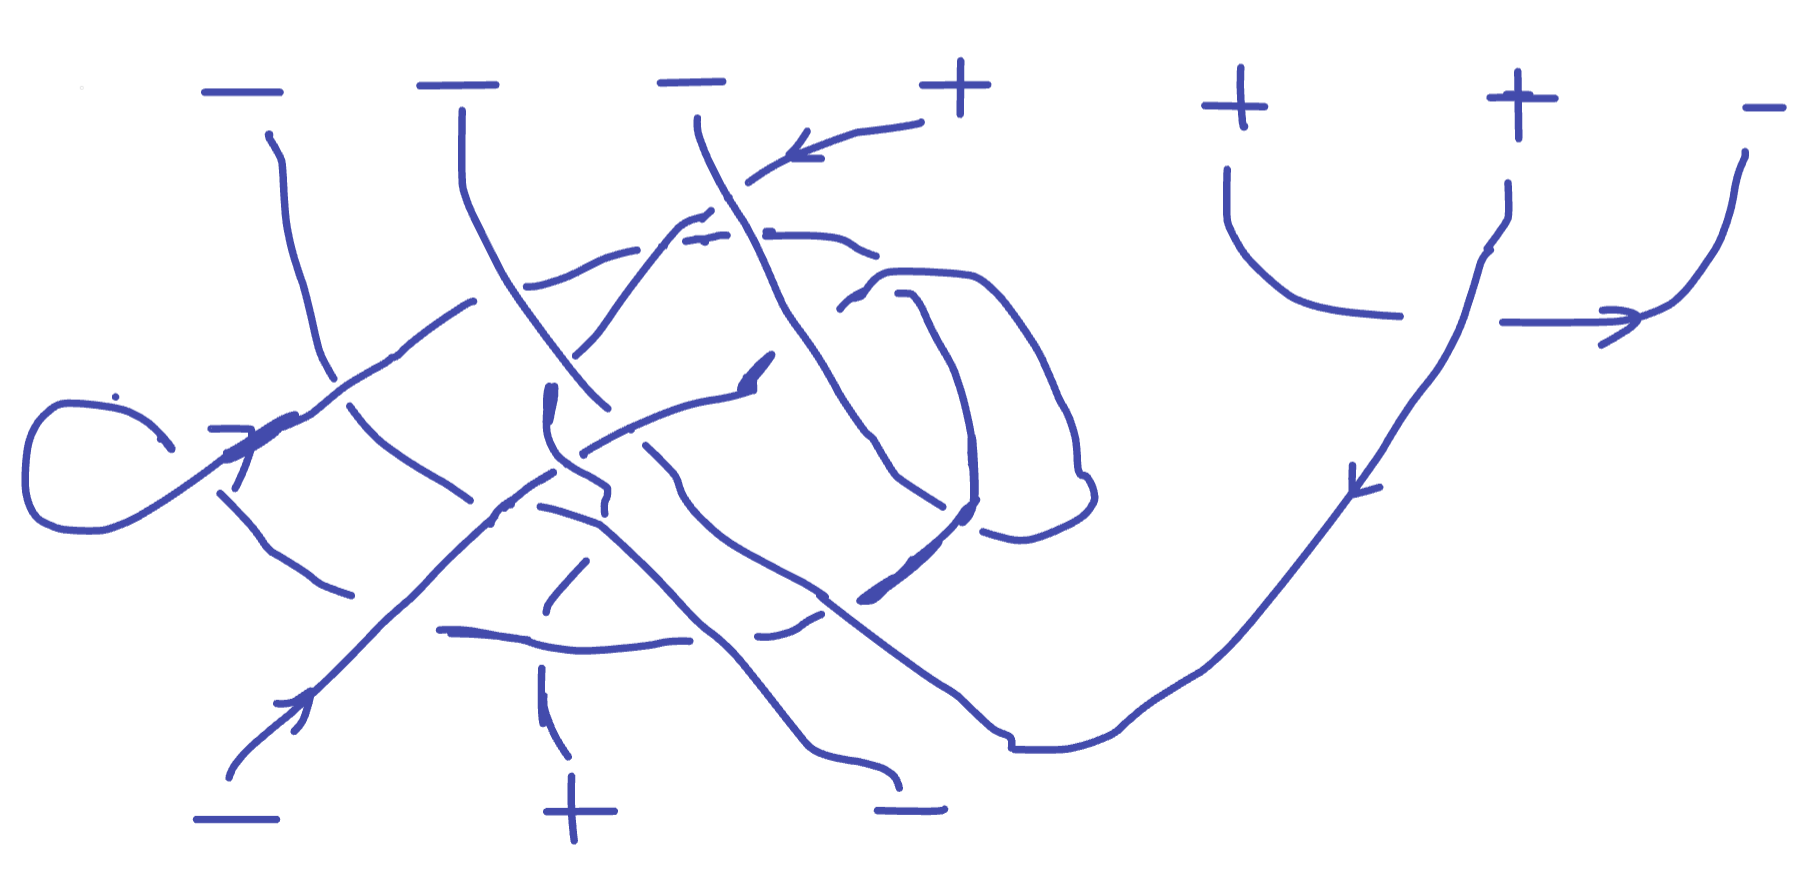
\includegraphics[scale=0.3]{tangle1.png}
    \end{center}

    Now we define the autonomous braided monoidal category $\mathcal{T}$ of tangles. The objects are functions $A : \{ 1, 2, \ldots, n \} \to \{ +, - \}$
    for $n \geq 0$ called \emph{signed sets}. The arrows of $\mathcal{T}$ are the tangles which have these signed sets as sources and targets. Composition
    and tensor-product are for braids. The braiding is visualised as follows:
    \begin{center}
    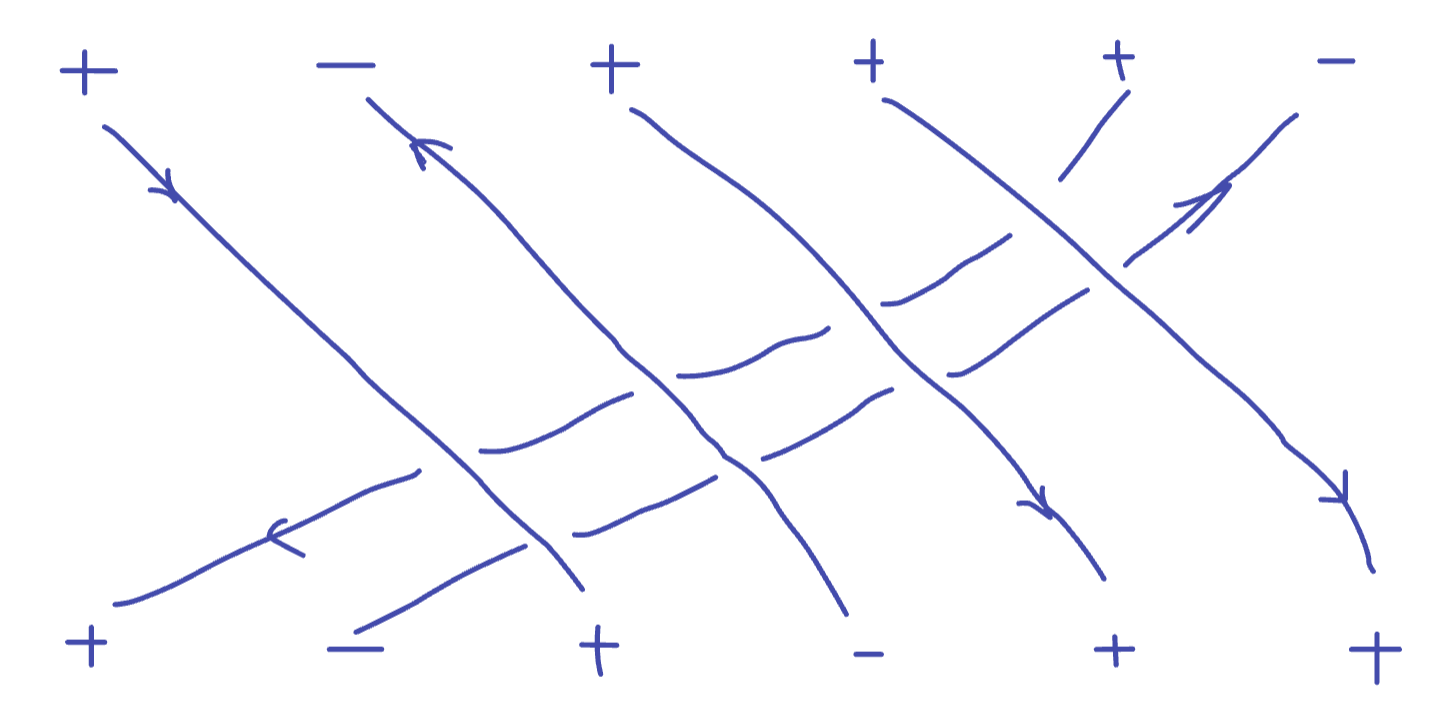
\includegraphics[scale=0.4]{tangle2.png}
    \end{center}
    The left dual $A^*$ of a signed set $A$ is given by reversing the order and the sign of the points. That is, $A^*(i)$ and $A(n - i + 1)$
    are opposite signs for $1 \leq i \leq n$. The counit and unit are illustrated below for $A = \{ -, +, -\}$:
    \begin{center}
    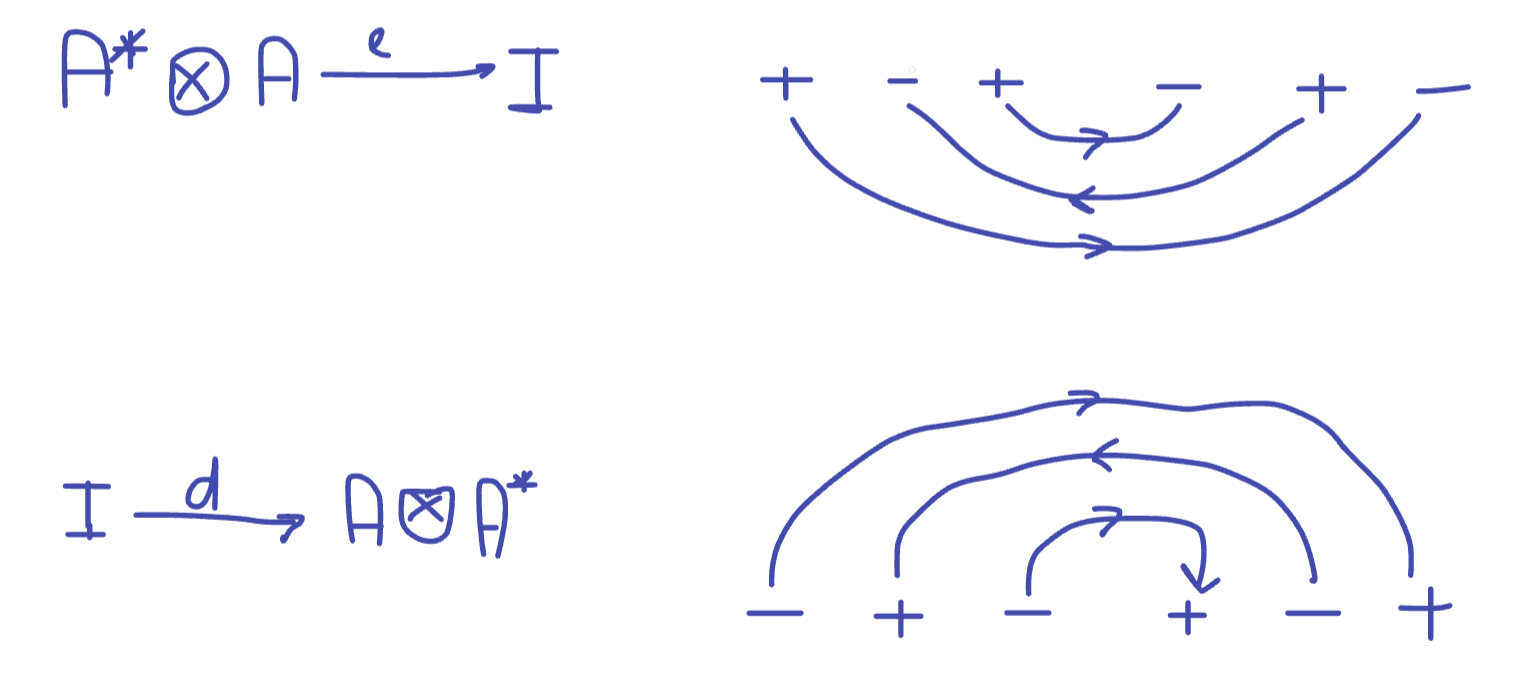
\includegraphics[scale=0.4]{tangle3.png}
    \end{center}
  \end{example}

  \section{Monoidal Functors and Yang-Baxter operators}
  Let $\mathcal{C}$ and $\mathcal{V}$ be monoidal categories. A \emph{monoidal functor} $F : \mathcal{C} \to \mathcal{V}$ consists of a functor $F : \mathcal{C} \to \mathcal{V}$
  along with a natural isomorphism $\phi_{A, B} : F A \otimes F B \xrightarrow{\cong} F(A \otimes B)$ and an isomorphism $\varphi_0 : I \xrightarrow{\cong} F I$ such
  that the following is satisfied:
  \[
  \begin{tikzcd}
    F A \otimes F B \otimes F C \ar[rr, "\phi_{A,B}"] \ar[dd, "1 \otimes \phi_{B,C}"'] && F (A \otimes B) \otimes F C \ar[dd, "\phi_{A \otimes B, C}"] & F A \ar[rr, "1 \otimes \varphi_0"] \ar[dd, "\varphi_0 \otimes 1"] \ar[ddrr, equal] && F A \otimes F I \ar[dd, "\varphi_{A,I}"]\\
    \\
    F A \otimes F (B \otimes C) \ar[rr, "\phi_{A, B \otimes C}"] && F (A \otimes B \otimes C)                                                          & F I \otimes F A  \ar[rr, "\varphi_{I,A}"']  && F A
  \end{tikzcd}
  \]
  If all the $\phi$'s are not invertible, then $F$ is a \emph{lax monoidal functor}; if $\phi$'s are identities, then $F$ is a \emph{strict monoidal functor}.

  If $\mathcal{C}$ and $\mathcal{V}$ are braided (symmetric), then a monoidal functor is braided (symmetric) if the following square commutes:
  \[
  \begin{tikzcd}
    F A \otimes F B \ar[rr, "\varphi_{A,B}"] \ar[dd, "c_{FA, FB}"] && F(A \otimes B) \ar[dd, "c_{FB, FA}"] \\
    \\
    F B \otimes F A \ar[rr, "\varphi_{B, A}"'] && F(B \otimes A)
  \end{tikzcd}
  \]
  If $\mathcal{C}$ and $\mathcal{V}$ are balanced, then $F$ is balanced if it is braided and $F(\theta_A) = \theta_{F A} : F A \to F A$.

  Let $F : \mathcal{C} \to \mathcal{V}$ is a lax monoidal functor and let $\mathcal{C}$ and $\mathcal{V}$ be left-closed, then the composite:
  \[
  F [A, B] \otimes F A \xrightarrow{\varphi_{[A,B], A}} F ([A, B] \otimes A) \xrightarrow{F e_A} F B
  \]
  corresponds to an arrow:
  \[
  \tilde{\phi_{A,B}} : F [A, B] \to [FA, FB]
  \]
  $F$ is a left-closed monoidal functor whenever each $\tilde{\phi_{A,B}}$ is invertible. Right-closed and closed are defined in a similar fashion.

  Note that monoidal functors preserve duals: if $F : \mathcal{C} \to \mathcal{V}$ is a monoidal functor and $d, e : B \dashv A$ in $\mathcal{C}$,
  then $F B \dashv F A$ in $\mathcal{V}$ with unit:
  \[
  I \xrightarrow{\phi_0} FI \xrightarrow{F d} F(B \otimes A) \xrightarrow{\phi^{-1}_{[A, B], A}} F A \otimes F B
  \]
  and counit
  \[
  F B \otimes F A \xrightarrow{\phi_{[B,A]}} F(B \otimes A) \xrightarrow{F e} FI \xrightarrow{\phi^{-1}_0} I
  \]

  \begin{example}
    The category ${\bf Set}$ of sets is a monoidal category with $\otimes = \times$. Let $R$ be a commutative ring, then the free module functor 
    $\mathcal{F}_R : {\bf Set} \to {\bf Mod}_R$ is monoidal. But it is not closed since:
    \[
    \operatorname{Hom}_R(\mathcal{F}_R X, \mathcal{F}_R Y) \cong (\mathcal{F}_R Y )^X \not\cong Y^X
    \]
    The functor $|\underline{\:\:}| : {\bf Mod}_R \to {\bf Set}$ taking a module $M$ to its underlying set $|M|$ is an example of a lax monoidal functor since the following functions:
    \begin{itemize}
      \item $\phi_{M,N} : |M| \times |N| \to |M \otimes N|$ with $(m,n) \mapsto m \otimes n$,
      \item $\phi_0 = \eta : 1 \mapsto |R|$.
    \end{itemize} 
  \end{example}

  \begin{example}
    The universal enveloping algebra functor $\mathcal{U} : {\bf Lie}_R \to {\bf Alg}_R$ is a monoidal functor.
  \end{example}

  \begin{example} Let $\mathcal{V}$ be a monoidal category.
    A \emph{Yang-Baxter operator} on an object $A \in \mathcal{V}$ is an invertible arrow $y : A \otimes A \to A \otimes A$ such that the following hexagon commutes:
    \[
    \begin{tikzcd}
    & A \otimes A \otimes A \ar[rr, "1 \otimes y"] && A \otimes A \otimes A \ar[dr, "y \otimes 1"] \\
    A \otimes A \otimes A \ar[ur, "y \otimes 1"] \ar[dr, "1 \otimes y"'] &&&& A \otimes A \otimes A \\
    & A \otimes A \otimes A \ar[rr, "y \otimes 1"'] && A \otimes A \otimes A \ar[ur, "1 \otimes y"'] \\
    \end{tikzcd}
    \]
    For instance, the object $1$ of $\mathcal{B}$ admits the following YB-operator:
    \[
    c_{1,1} = s_1 : 1 + 1 \to 1 + 1
    \]
    which is the element of the braid group $\mathcal{B}_2$:
    \begin{center}
    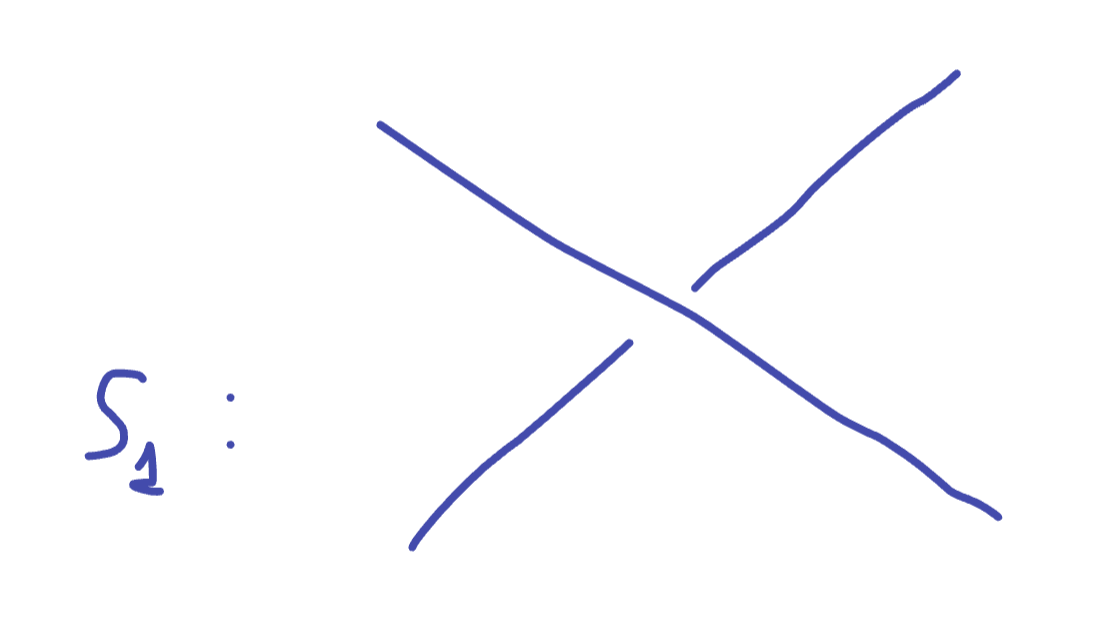
\includegraphics[scale=0.3]{yb1.png}
    \end{center}
    Then the YB-hexagon becomes the following identity:
    \begin{center}
    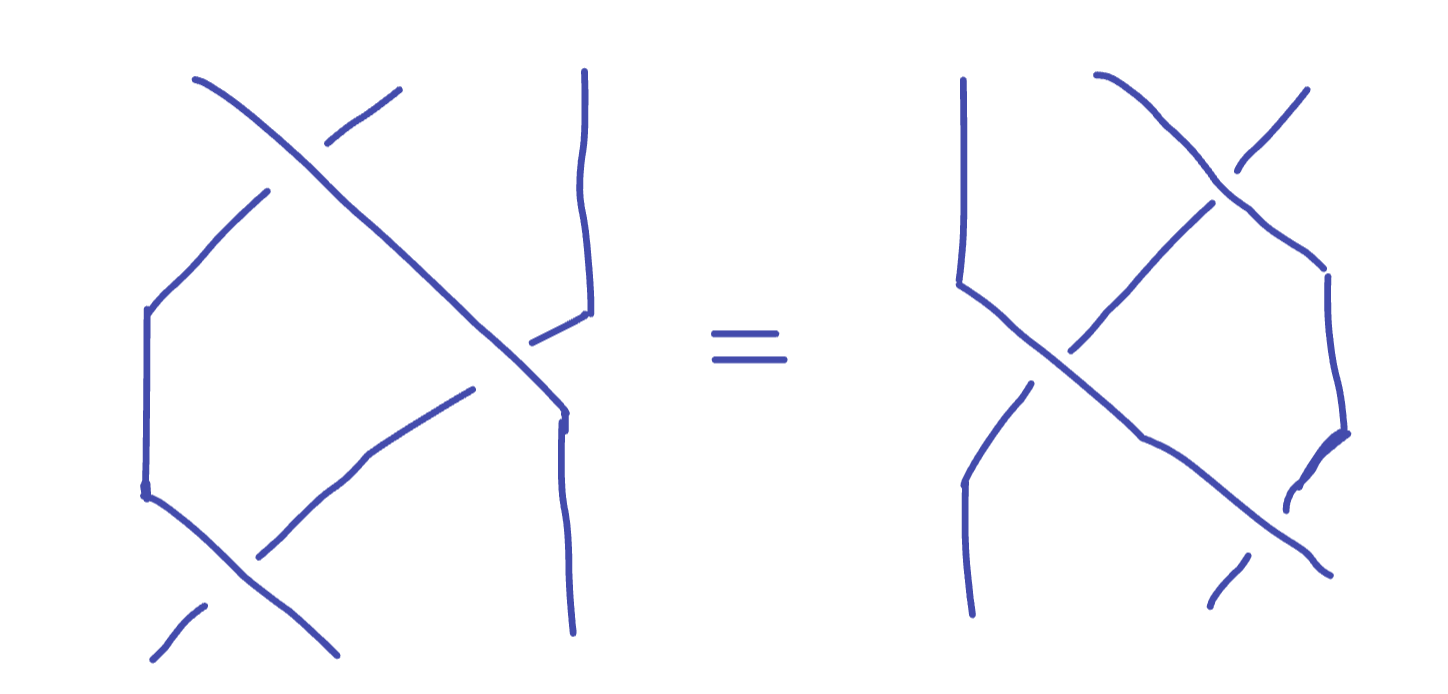
\includegraphics[scale=0.3]{yb2.png}
    \end{center}
    As far as monoidal functor $F : \mathcal{B} \to \mathcal{V}$ preserves tensors up to isomorphism, one obtains a YB-operator $y$ on $F(1) = A$:
    \[
    y : A \otimes A \xrightarrow{\phi_{1,1}} F(1 + 1) \xrightarrow{F s_1} F(1 + 1) \xrightarrow{\phi^{-1}_{1,1}} A \otimes A
    \]

    Given a YB-operator $y$ on $A \in \mathcal{V}$, one can determine a monoidal functor $F : \mathcal{B} \to \mathcal{V}$ such that $F(1) = A$ and $y$ is the above composite.
    Moreover, $F$ is unique up to isomorphism. As far as $F$ is a monoidal functor, we also have:
    \[
    F(n) = F(1 + 1 + \ldots + 1) \cong A^{\otimes n}
    \]
    Each generator $s_i$ of $\mathcal{B}_n$ can be written as
    \[
    s_i = {\bf 1}_{i - 1} \otimes s_1 \otimes {\bf 1}_{n - i - 1} \in \mathcal{B}
    \]
    Thus, the definition of $F s_i : A^{\otimes n} \to A^{\otimes n}$ is forced.
  \end{example}
  \begin{example}
    A tensor functor from ribbons $F : \tilde{\mathcal{B}} \to \mathcal{V}$ determines a $YB$-operator $y$ on $F1 = A$ as in the above example. 
    The twist $\theta_1 : 1 \to 1$ in $\tilde{\mathcal{B}}$ gives an isomorphism $z = F\theta_1 : A \to A$.
    Due to the following equalities in $\tilde{\mathcal{B}}$:
    \begin{center}
    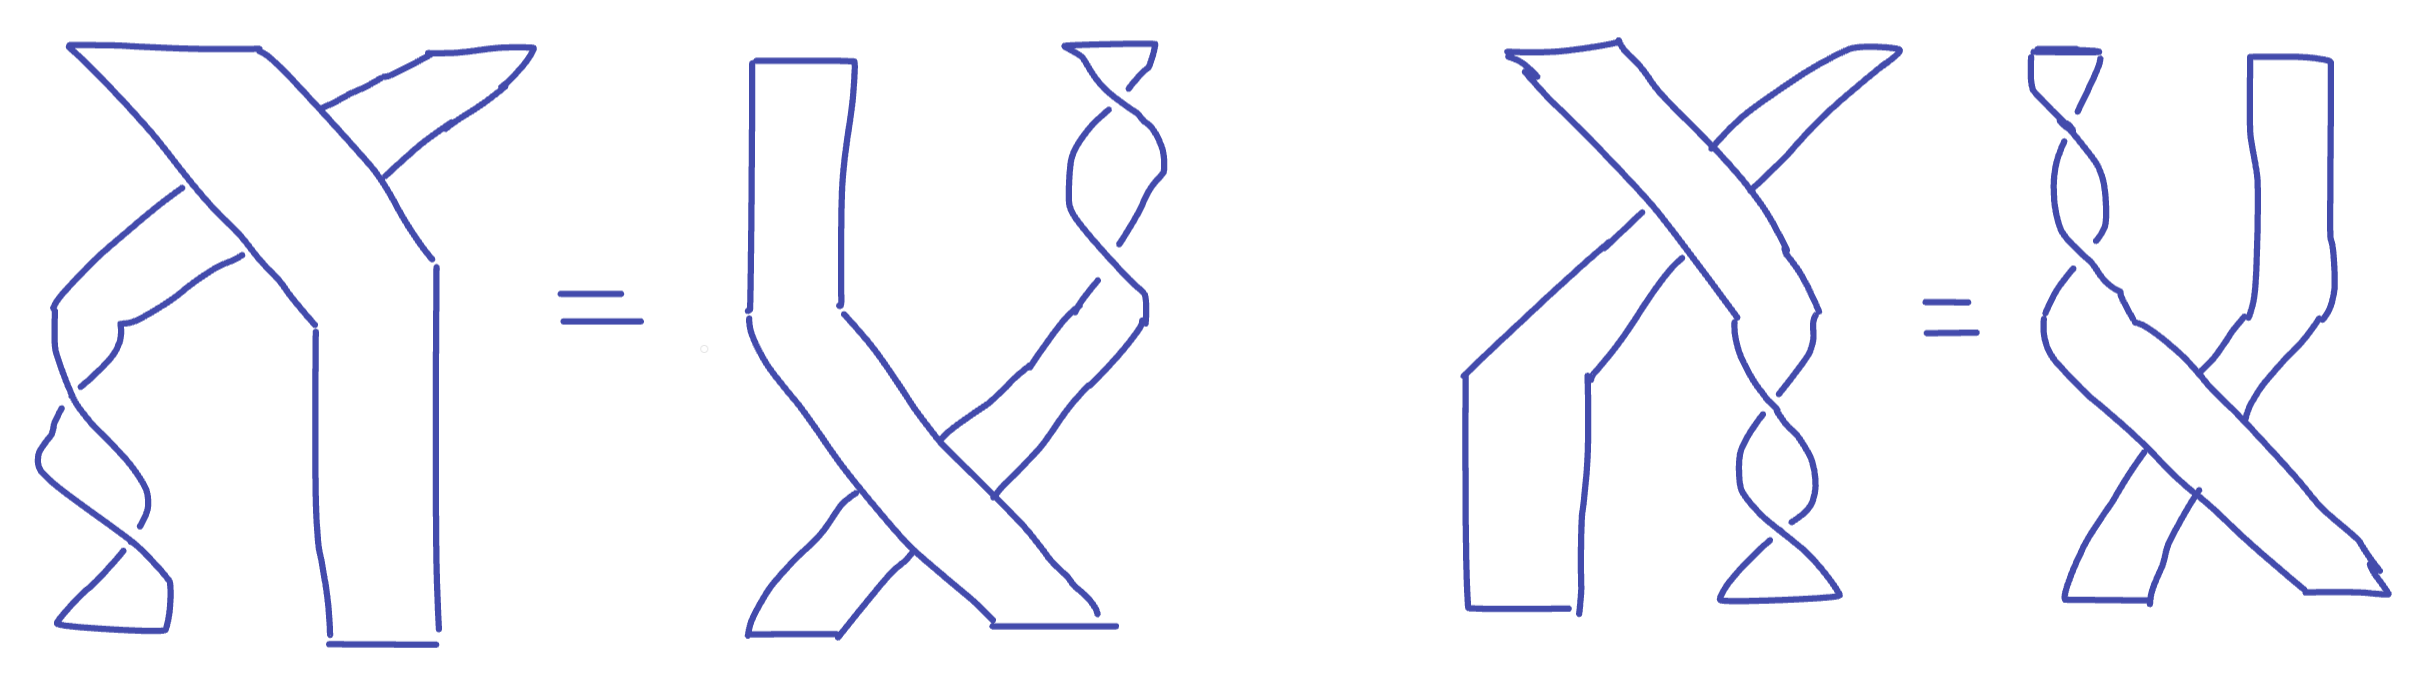
\includegraphics[scale=0.3]{yb3.png}
    \end{center}
    A YB-operator $y$ on an object $A \in \mathcal{V}$ is \emph{balanced} when it is equipped with an isomorphism $z : A \to A$ such that the following squares commute:
    \[
    \begin{tikzcd}
      A \otimes A \ar[rr, "y"] \ar[dd, "1 \otimes z"'] && A \otimes A \ar[dd, "z \otimes 1"] & A \otimes A \ar[rr, "y"]  \ar[dd, "z \otimes 1"']  && A \otimes A \ar[dd, "1 \otimes z"] \\
      \\
      A \otimes A \ar[rr, "y"'] && A \otimes A & A \otimes A \ar[rr, "y"'] && A \otimes A
    \end{tikzcd}
    \]
    Each balanced YB-operator determines a unique monoidal functor $F : \tilde{\mathcal{B}} \to \mathcal{V}$ from which $A$, $y$ and $z$ are recovered. Therefore,
    $(\tilde{B}, 1, c_{1,1}, \theta_1)$ is the free tensor category containing an object equipped with a balanced YB-operator.
  \end{example}
  Let us recall the following observations:
  \begin{itemize}
    \item Monoidal functors take YB-operators to YB-operators.
    \item A braiding on each monoidal category gives a YB-operator $c_{A,A} : A \otimes A \to A \otimes A$.
  \end{itemize}
  Besides, monoidal functors take balanced YB-operators to balanced YB-operators.

  A YB-operator $y$ on $A$ is called (\emph{left}-) \emph{dualisable} when $A$ has a left dual $A^*$ and both the arrows $u, v : A^* \otimes A \to A^*$ are given by the composites:
  \[
  \begin{tikzcd}
    A^* \otimes A \ar[rr, "1 \otimes 1 \otimes d"] && A^* \otimes A \otimes A \otimes A^* \ar[rr, shift left, "1 \otimes y \otimes 1"] \ar[rr, shift right, "1 \otimes y^{-1} \otimes 1"'] && A^* \otimes A \otimes A \otimes A^* \ar[rr, "e \otimes 1 \otimes 1"] && A \otimes A^*
  \end{tikzcd}
  \]
  are invertible. It follows that the composite $w$ given by:
  \[
  \begin{tikzcd}
    A^* \otimes A^* \ar[rr, "1 \otimes 1 \otimes d"] && A^* \otimes A^* \otimes A \otimes A^* \ar[rr, "1 \otimes u \otimes 1"] && A^* \otimes A \otimes A^* \otimes A^* \ar[rr, "e \otimes 1 \otimes 1"] && A^* \otimes A^*
  \end{tikzcd}
  \]
  has inverse $w^{-1}$ given by the following composite:
  \[
  \begin{tikzcd}
    A^* \otimes A^* \ar[rr, "1 \otimes 1 \otimes d"] && A^* \otimes A^* \otimes A \otimes A^* \ar[rr, "1 \otimes v \otimes 1"] && A^* \otimes A \otimes A^* \otimes A^* \ar[rr, "e \otimes 1 \otimes 1"] && A^* \otimes A^*
  \end{tikzcd}
  \]
  \begin{prop}
    In a braided monoidal category, if an object $A$ has a dual, then $y = c_{A,A}$ is a dualisable YB-operator on $A$ with:
    \[
    u = c^{-1}_{A,A^*}, v = c^{-1}_{A^*,A}, w = c^{-1}_{A^*,A^*}.
    \]
  \end{prop}
  \begin{proof}
    $c^{-1}_{A,A^*} \circ u = 1_{A^* \otimes A}$, it suffices to show that equality holds after applying $A \otimes \underline{\:\:}$ to both sides and composing
    with $d \otimes 1_A$. The following diagram gives the first equation:
    \begin{small}
    \[
    \begin{tikzcd}
      A \otimes A^* \otimes A \otimes A \otimes A^* \ar[rrrrrr, "1 \otimes 1 \otimes c_{A,A} \otimes 1"] &&&&&& A \otimes A^* \otimes A \otimes A \otimes A^* \ar[dd, "1 \otimes e \otimes 1 \otimes 1"] \\
      \\
      A \otimes A^* \ar[uu, "1 \otimes 1 \otimes 1 \otimes d"] \otimes A && |[alias=AAA*]| A \otimes A \otimes A^* \ar[uull, "d \otimes 1 \otimes 1 \otimes 1"] \ar[rr, "c_{A,A} \otimes 1"] && A \otimes A \otimes A^* \ar[rr, equal] \ar[uurr, "d \otimes 1 \otimes 1 \otimes 1"] && A \otimes A \otimes A^* \ar[dd, "1 \otimes c_{A,A^*}"] \\
      \\
      A \ar[rrr, equal] \ar[uurr, "1 \otimes d"] \ar[uu, "d \otimes 1"] &&& A \ar[rrr, "d \otimes 1"'] &&& |[alias=AA*A]| A \otimes A^* \otimes A
      \ar[from=AAA*,to=AA*A, "c_{A, A \otimes A^*}"]
    \end{tikzcd}
    \]
  \end{small}
  The other equalities are shown similarly.
  \end{proof}
  Monoidal functors preserve dualisability: if $\mathcal{C}$ is braided and $X$ has a dual in $\mathcal{V}$, we obtain a dualisable YB-operator $F X$ in $\mathcal{V}$.

  A YB-operator on A is called \emph{tortile} when it is balanced, dualisable and the following diagram commmutes:
  \[
  \begin{tikzcd}
    && A \otimes A \otimes A^* \ar[dr, "1 \otimes v^{-1}"] \\
    & A \otimes A \otimes A^* \ar[ur, "y \otimes 1"] && A \otimes A^* \otimes A \ar[dr, "1 \otimes e"] \\
    A \ar[rr, "z"'] \ar[ur, "1 \otimes d"] && A \ar[rr, "z"'] && A
  \end{tikzcd}
  \]
  \begin{prop}
    In a balanced monoidal category, if an object $A$ has a dual then the pair $(c_{A,A}, \theta_A)$
    is a tortile YB-operator precisely when:
    \[
    \theta_{A^*} = (\theta_A)^*.
    \]
  \end{prop}
  \begin{proof}
    The following equation:
    \[
    (\theta_{A^*})^* \theta_A = (1 \otimes e) \circ (1 \otimes v^{-1}) \circ (y \otimes 1) \circ (1 \otimes d)
    \]
    is proved by the following diagram:
    \[
    \begin{tikzcd}
      A \ar[rr, "\theta_A"] \ar[dd, "1 \otimes d"'] && A \ar[rr, "1 \otimes d"] && A \otimes A \otimes A^* \ar[rr, "1 \otimes c^{-1}_{A^*,A}"] && A \otimes A^* \otimes A \ar[dd, "1 \otimes \theta_{A^*} \otimes 1"] \\
      \\
      A \otimes A \otimes A^* \ar[ddrr, "c^{-1}_{A^*,A}"] \ar[rrrr, "1 \otimes c^{-1}_{A^*,A}"] \ar[dddddd, "y \otimes 1 = c_{A,A} \otimes 1"'] &&&& A \otimes A^* \otimes A \ar[ddll, "c^{-1}_{A^*,A} \otimes 1"'] \ar[rr, "\theta_A \otimes \theta_{A^*} \otimes 1"'] \ar[uurr, "\theta_A \otimes 1 \otimes 1"] && A \otimes A^* \otimes A \ar[dd, "c^{-1}_{A,A^*} \otimes 1"]\\
      \\
      && A^* \otimes A \otimes A \ar[rrrr, "\theta_{A^* \otimes A} \otimes 1"] \ar[ddddrr, "c_{A^* \otimes A,A}"] \ar[dd, "1 \otimes c_{A,A}"'] \ar[ddrr, "e \otimes 1"] &&&& A^* \otimes A \otimes A \ar[dd, "e \otimes 1"] \\
      \\
      && A^* \otimes A \otimes A \ar[ddrr, "c_{A^*,A} \otimes 1"'] && A \ar[rr, equal] \ar[ddrr, equal] && A \ar[dd, equal] \\
      \\
      A \otimes A \otimes A^* \ar[uurr, "c^{-1}_{A^*,A \otimes A}"] \ar[rrrr, "1 \otimes v^{-1} = 1 \otimes c^{-1}_{A^*,A}"'] &&&& A \otimes A^* \otimes A \ar[rr, "1 \otimes e"'] && A
    \end{tikzcd}
    \]
    Thus the balanced YB-operator $(y,z)$ is tortile if and only if $(\theta_{A^*})^* \theta_A = z^2$, i.e., if and only
    if
    \[
    (\theta_{A^*})^* \theta_A = (\theta_A)^2 \Leftrightarrow (\theta_{A^*})^* = \theta_A \Leftrightarrow \theta_{A^*} = (\theta_A)^*.
    \]
  \end{proof}
  Therefore, in a tortile monoidal category each object $A$ is equipped with a tortile YB-operator $(c_{A,A}, \theta_A)$.
  \begin{example}
    As far as $\tilde{\mathcal{T}}$ is a tortile monoidal category, we obtain a tortile YB-operator $(c_{+,+}, \theta_+)$ on the object $+$ of
    $\tilde{\mathcal{T}}$. Thus, each monoidal functor $F : \tilde{\mathcal{T}} \to \mathcal{C}$ yields a tortile YB-operator on $F(+)$ in $\mathcal{V}$.

    $(\tilde{\mathcal{T}}, +, c_{+,+}, \theta_+)$ is the free monoidal category equipped with a tortile YB-operator.
    This means the following thing. Let $(y,z)$ be a tortile YB-operator on $A$ in a monoidal category $\mathcal{V}$,
    then there is a unique up to isomorphism monoidal functor $F : \tilde{\mathcal{T}} \to \mathcal{V}$ such that:
    \[
    F : (+, c_{+,+}, \theta_+) \mapsto (A, y, z).
    \]
    This is how $F$ is defined in terms of $A, y, z$. For example:
    \begin{itemize}
      \item $F(+---+-) = A \otimes A^* \otimes A^* \otimes A^* \otimes A \otimes A^*$,
      \item $F(c_{+,-}) = u^{-1}$,
      \item $F(c_{-,-}) = w$,
      \item $F(\theta_+) = z$,
      \item $F(\theta_{-}) = z^*$.
      \item etc.
    \end{itemize}
    Any tangle of ribbons can be decomposed, using composition and tensor product in $\tilde{\mathcal{T}}$,
    into single crossings ($c_{+, +}$, $c_{+,-}$, $c_{-,+}$, $c_{-,-}$ and their inverses), turnings $e$ and $d$ and
    twists ($\theta_{+}$, $\theta_{-}$ and their inverses). Thus the value of $F$ is forced.
  \end{example}
\end{document}